\documentclass[]{article}
\usepackage{lmodern}
\usepackage{amssymb,amsmath}
\usepackage{ifxetex,ifluatex}
\usepackage{fixltx2e} % provides \textsubscript
\ifnum 0\ifxetex 1\fi\ifluatex 1\fi=0 % if pdftex
  \usepackage[T1]{fontenc}
  \usepackage[utf8]{inputenc}
\else % if luatex or xelatex
  \ifxetex
    \usepackage{mathspec}
  \else
    \usepackage{fontspec}
  \fi
  \defaultfontfeatures{Ligatures=TeX,Scale=MatchLowercase}
  \newcommand{\euro}{€}
\fi
% use upquote if available, for straight quotes in verbatim environments
\IfFileExists{upquote.sty}{\usepackage{upquote}}{}
% use microtype if available
\IfFileExists{microtype.sty}{%
\usepackage{microtype}
\UseMicrotypeSet[protrusion]{basicmath} % disable protrusion for tt fonts
}{}
\usepackage[margin=1in]{geometry}
\usepackage{hyperref}
\PassOptionsToPackage{usenames,dvipsnames}{color} % color is loaded by hyperref
\hypersetup{unicode=true,
            pdftitle={Estimating the effect of state-level gun purchasing policy on county-level firearm suicide mortality},
            pdfauthor={Timothy M Wolock},
            pdfborder={0 0 0},
            breaklinks=true}
\urlstyle{same}  % don't use monospace font for urls
\usepackage{longtable,booktabs}
\usepackage{graphicx,grffile}
\makeatletter
\def\maxwidth{\ifdim\Gin@nat@width>\linewidth\linewidth\else\Gin@nat@width\fi}
\def\maxheight{\ifdim\Gin@nat@height>\textheight\textheight\else\Gin@nat@height\fi}
\makeatother
% Scale images if necessary, so that they will not overflow the page
% margins by default, and it is still possible to overwrite the defaults
% using explicit options in \includegraphics[width, height, ...]{}
\setkeys{Gin}{width=\maxwidth,height=\maxheight,keepaspectratio}
\setlength{\parindent}{0pt}
\setlength{\parskip}{6pt plus 2pt minus 1pt}
\setlength{\emergencystretch}{3em}  % prevent overfull lines
\providecommand{\tightlist}{%
  \setlength{\itemsep}{0pt}\setlength{\parskip}{0pt}}
\setcounter{secnumdepth}{0}

%%% Use protect on footnotes to avoid problems with footnotes in titles
\let\rmarkdownfootnote\footnote%
\def\footnote{\protect\rmarkdownfootnote}

%%% Change title format to be more compact
\usepackage{titling}

% Create subtitle command for use in maketitle
\newcommand{\subtitle}[1]{
  \posttitle{
    \begin{center}\large#1\end{center}
    }
}

\setlength{\droptitle}{-2em}
  \title{Estimating the effect of state-level gun purchasing policy on
county-level firearm suicide mortality}
  \pretitle{\vspace{\droptitle}\centering\huge}
  \posttitle{\par}
  \author{Timothy M Wolock}
  \preauthor{\centering\large\emph}
  \postauthor{\par}
  \predate{\centering\large\emph}
  \postdate{\par}
  \date{June 30, 2016}



% Redefines (sub)paragraphs to behave more like sections
\ifx\paragraph\undefined\else
\let\oldparagraph\paragraph
\renewcommand{\paragraph}[1]{\oldparagraph{#1}\mbox{}}
\fi
\ifx\subparagraph\undefined\else
\let\oldsubparagraph\subparagraph
\renewcommand{\subparagraph}[1]{\oldsubparagraph{#1}\mbox{}}
\fi

\begin{document}
\maketitle

{
\setcounter{tocdepth}{2}
\tableofcontents
}
\pagebreak

\section{Introduction}\label{introduction}

\subsection{Background}\label{background}

In the wake of several highly publicized mass shootings, gun control has
become one of the most divisive issues in American politics. Most
recently, the murder of 49 people at a nightclub in Orlando, Florida has
sparked a national debate about how and whether or not such events can
be prevented in the future.\textsuperscript{1} This debate echoes the
one after the 2013 shooting at Sandy Hook Elementary School in Newtown,
Connecticut in which a gunman murdered 20 children and six
adults.\textsuperscript{2} That event catalyzed an effort by Democrats
in the federal government to severely restrict access to military-style
rifles and to limit the legal size of ammunition
magazines.\textsuperscript{3} Ultimately, each of those bills was
rejected by Senate Republicans, but their shared goal (to prevent mass
shootings) was reflective of the public discourse at the time.

However, this focus is not reflective of the true burden of gun violence
in America. According to the US Centers for Disease Control and
Prevention (CDC) nearly two-thirds of annual firearm deaths in the US
(roughly 21,000 of 33,000 in 2013) are intentional
self-harm.\textsuperscript{4,5} Just under one-third of the remainder
are homicides, and the rest (approximately 4\%) are classified as
accidental.\textsuperscript{6} The CDC reports that slightly more than
one-half of all suicides in the US were committed with a firearm, so any
suite of gun control policies that does not include interventions
specifically designed to prevent suicide (such as the one proposed after
the Sandy Hook shooting) will leave the actual source of most firearm
deaths unaddressed.

Although gun violence is typically framed in criminological terms in the
US, when we compare gun violence mortality rates in the US to rates in
other countries, the need for a public health approach becomes clear. In
2013, the United States experienced a firearm mortality rate of 10.6
deaths per 100,000 people.\textsuperscript{5} This stands in stark
contrast to the rate of death by firearm injury in every other developed
country. Finland had the second highest rate in recent years: 3.6 deaths
per 100,000 people in 2010, which is slightly more than one-third the
American rate in 2013.\textsuperscript{7} In Canada in 2011, the
mortality rate due to gun violence was 2.1 deaths per 100,000 people,
just under one-fifth the US rate.\textsuperscript{8} The US is an
extraordinary outlier among its economic peers in terms of firearm
mortality.

Efforts to rein in gun violence in the US typically take the form of
federal- and state-level restrictions on firearm purchasing and
ownership commonly referred to as ``gun control.'' Several broad laws
(most notably, the Brady Bill and the Federal Assault Weapons Ban) have
been implemented by the federal government, but states have substantial
latitude in regulating gun sales and ownership outside of the scope of
federal regulation. The Brady Bill mandated federal background checks of
all firearm purchasers in the United States and established a mandatory
five-day waiting period on purchases.\textsuperscript{9} It was
effective until 1998 when the National Instant Background Check System
was implemented. Similarly, the Federal Assault Weapons Ban outlawed
ownership of ``assault weapons'' and ``large capacity'' ammunition
magazines, but it expired in 2004 and has not been
renewed.\textsuperscript{10} Both of these bills were designed with the
intention of preventing homicide, not suicide.

At the state-level, we see enormous variation in gun control policies.
Whereas several allow concealed carry of firearms on public university
campuses, Governor Jay Inslee of Washington state has launched a highly
publicized public health capaign to fight gun
violence.\textsuperscript{11} At an even more granular level, some
individual counties and municipalities have enacted their own gun
control measures. For instance, handgun sales were illegal in Chicago,
Illinois until 2013.\textsuperscript{12} Many states have passed
``preemption'' laws that prevent smaller governments within the state
from passing more severe gun control laws than the state
legislature.\textsuperscript{13} Despite this smaller-scale variation,
most direct gun control policymaking is done in state legislatures.

However, the effectiveness of these laws is all but completely unknown
because the epidemiological dynamics of gun violence are poorly
understood at best. After Kellermann \emph{et al.} published their study
identifying firearm ownership as a risk factor for homicide in 1993, the
National Rifle Association (NRA) began a lobbying campaign to defund the
CDC's National Center for Injury Prevention.\textsuperscript{14,15} That
effort failed, but, working with House Representative Jay Dickey, an
amendment was inserted into the 1996 Omnibus Consolidated Appropriations
Bill that prevented the CDC from using any of its injury prevention
funding in FY 1997 for the promotion of gun control. This amounted to a
ban on gun violence research that persists to this day.

The result of this ban has been a near-total drought of published
research on gun violence prevention, making evidence-based policymaking
impossible. The national debate around one of the most controversial
political issues in modern American politics is fueled by anecdotes and
untested theories. The popular discourse around suicide is particularly
unproductive. There is a widespread perception of suicide as inevitable,
leading to its dismissal as a preventable public health crisis. Gun
rights advocates argue that gun control cannot prevent suicide because
people who cannot access a firearm to commit suicide will just commit
suicide using some other method.\textsuperscript{16--18} This
substitution hypothesis warrants particular scrutiny because firearms
are far and away the most lethal means of attempting
suicide.\textsuperscript{19}

In summary, most of the public discussion of gun control centers around
mass shootings, but the largest source of health loss from firearms is
suicide. However, the epidemiology of gun violence is poorly understood
at best, making evidence-based decision making impossible.

\subsection{Research Question}\label{research-question}

In this study, we attempted to test the theory that particular gun
control policies were effective in reducing firearm suicide mortality
rates. We sought to help inform one of the most contentious debates in
American politics and to fill the substantial data gaps in the rapidly
growing field of gun violence research. More specifically, we chose to
estimate the effect of handgun permit-to-purchase (PTP) requirements on
firearm suicide mortality. PTP requirements mandate that all potential
handgun purchasers at certified sellers must present a permit or license
issued by the state. We focused on this one policy for several reasons.
First, it has been identified as an important item in the existing set
of gun control policies by advocacy gropus on both sides of the
issue.\textsuperscript{20} Second, requiring potential handgun
purchasers to have already acquired a state-issued permit fits neatly
into the model of gun control as a suicide prevention tool. Finally and
most practically, it was only possible to research the legislative
history of one policy for all fifty states.

We can rephrase this question quantitatively: Do policies requiring
potential handgun purchasers to have a state-issued permit or license
significantly reduce firearm suicide mortality? We hypothesized that
these laws were effective and that we would observe significantly lower
firearm suicide mortality in places with such requirements.

As a secondary analysis, we examined the previously discussed
substitution hypothesis by trying to identify any effect handgun
purchasing permit requirements had on suicide by all non-firearm means
and whether this substitution effect negated the benefits of the law.
Given the relatively high lethality of firearms as a means of attempting
suicide, we hypothesized that we would not see an increase in suicide by
other means and that, if we did, it would be outweighed by the observed
benefits. Even if every person who could not get access to a firearm for
suicide attempted suicide by some other means, we would still expect to
see a net benefit.

\subsection{Literature Review}\label{literature-review}

The existing body of literature examining the public health effects of
gun control is relatively small given the scale of the problem. Several
studies have examined the relationship between handgun purchasing
policies and firearm mortality. Webster \emph{et al.} used generalized
least squares regression models to estimate the effect of Missouri's
2007 repeal of its PTP requirement on mortality.\textsuperscript{21}
They found that it corresponded with a significant 23\% increase in
annual firearm homicide rates. Rudolph \emph{et al.} used a ``synthetic
control method,'' which uses comparable states as artificial controls,
to find that Connecticut's 1995 implementation of a PTP law was
associated with a 40\% decrease in firearm homicide mortality over the
course of 10 years.\textsuperscript{22} In a 2015 study that also used a
synthetic control method, Crifasi \emph{et al.} associated Connecticut's
implementation of a PTP law with a 15.4\% reduction in firearm suicide
rates and Missouri's repeal of its law with a 16.1\% increase in firearm
suicide rates.\textsuperscript{23} Anestis \emph{et al.} found that
states with PTP requirements experienced significantly lower firearm
suicide mortality in 2013 than states without PTP
requirements.\textsuperscript{24}

Although all of these studies found substantial and significant effects,
their designs severely limit the extent to which we can infer that their
results are causal. Webster \emph{et al.} and Anestis \emph{et al.} both
parameterized the exposure variable as a state-year specific binary
based on whether that particular state had a PTP law in that year. In
the case of Webster \emph{et al.}, this means that the authors
identified a significant discontinuity in the level of firearm homicide
mortality before and after the policy, but this change could easily be
attributable to another policy change in a similar year or to a more
gradual social process that had been in the process for years. In the
case of Anestis \emph{et al.}, the authors only used data from 2010,
meaning that the differences they capture between states could easily be
a result of more abstract cultural factors, not any particular policy.
The synthetic control approach used by Rudolph \emph{et al.} and Crifasi
\emph{et al.} is vulnerable to similar problems. Its validity depends
entirely on the appropriateness of the controls used to generate the
synthetic counterfactual series, so, as with the binary exposure
variable, it is difficult to say that the model is capturing the effect
of one particular policy or another.

Several other studies have looked more generally at the health effects
of gun control or at other particular policies. In order to create more
variation across states in the exposure variable and to avoid bias due
to co-occurence of laws, many studies collect laws into legislative
strength scores. Since 2007 the Law Center to Prevent Gun Violence and
the Brady Campaign to Prevent Gun Violence have produced a state gun law
scorecard that assigns higher numeric and letter grades to states with
more (and more ``effective'') gun control laws. Fleegler \emph{et al.}
found that, between 2007 and 2010, states in the highest quartile of
this score had significantly lower overall firearm mortality, homicide
firearm mortality, and suicide firearm mortality than states in the
bottom quartile.\textsuperscript{25} Kposowa \emph{et al.} found that a
score from the same source as Fleegler \emph{et al.} was significantly
and negatively associated with state-level firearm suicide mortality
between 2011 and 2013.\textsuperscript{26} Rodríguez Andrés \emph{et
al.} constructed a time series of scores based on several tiers of
legislative strength from 1995 through 2004 and found that it was
significantly associated with decreased rates of firearm suicide in
men.\textsuperscript{27} They also found that several individual
policies (including PTP requirements) had significant effects.

The composite metrics described above are useful for adding variation
between states in analyses with no structure related to time, but the
weighting schemes they use are essentially arbitrary. In fact, because
the epidemiology of gun violence in the US is so poorly understood,
informing these schemes with evidence seems circular. In response to
this, Kalesan \emph{et al.} estimated the effects of 25 state laws
independently on overal firearm mortality in 2009.\textsuperscript{28}
They found that nine of the identified laws were associated with
decreased firearm mortality, nine were associated with increased firearm
mortality, and seven were inconclusive. However their study exhibits
flaws similar to those we observed in Anestis \emph{et al.}.

In general, the rapidly developing body of research on the effects of
gun control in the US seems to suggest that more restrictive gun control
leads to lower firearm mortality. However, most of these studies are
designed in ways that severely cripple their causal validity. The set of
exposure parameterizations that have been used previously all have the
potential to capture essentially irrelevant cultural variation instead
of the causal effect of a policy.

\subsection{Conceptual Model}\label{conceptual-model}

We based our conceptual model on the ``cry of pain'' model of
suicidality, which frames suicidal behavior as a response to stressful
situations. These stressful situations have three components that fuel
suicidal ideation: presence of defeat, preception of no escape, and
perception of no rescue. Stark \emph{et al.} extended this simple model
to include societal and environmental factors.\textsuperscript{29} Our
conceptual model, based on the one proposed by Stark \emph{et al.}, is
presented in Figure 1

\begin{figure}[htbp]
\centering
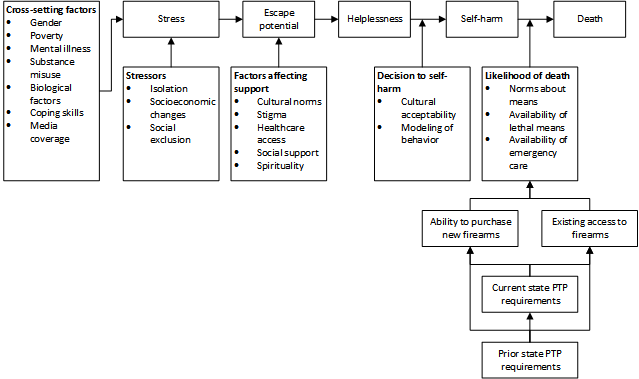
\includegraphics{Conceptual_model.png}
\caption{Conceptual model of PTP requirement as suicide prevention tool}
\end{figure}

The model theorizes that a PTP requirement can prevent firearm suicide
deaths in two distinct ways, both of which involve limiting access to
firearms. First, by making purchasing handguns less convenient, a PTP
law should prevent some number of handgun purchases from ever happening.
This should reduce the probability than any given individual
experiencing suicidal ideation already has access to a handgun. Second,
a PTP requirement drastically reduces an individual's ability to
purchase a handgun spontaneously, preventing some number of individuals
from purchasing handguns for the express purpose of attempting suicide.

The model also encompasses the theorized mechanism by which individuals
who cannot access a firearm for a suicide attempt find some other means
to attempt suicide. Having been unable to access a firearm, individuals
select some other means and, based on the lethality of the alternative
method, either complete or do not complete their attempt.

Most importantly, this model frames suicide prevention in terms of
single individuals' suicidal episodes; an individual's probability of
dying as a result of a single suicide attempt is a function of (among
other factors) the current availability of different means. We expect
that the effectiveness of a PTP requirement at reducing the number of
handguns in the population will wane over time as guns are purchased in
settings not covered by the law (at gun shows, in other states,
illegally, etc.). The binary exposure variable used in many of the
studies discussed above does not allow for this possibility; it assumes
that the effect is constant post-law. If PTP requirements are variably
effective over time at reducing the number of guns in the population,
then we would actually expect the observed effect on firearm suicide
mortality to exhibit a relatively smooth pattern of policy-time.

\section{Methods}\label{methods}

We used a sex-specific linear regression with a Poisson likelihood to
assess the effect of PTP requirements on firearm suicide mortality,
suicide mortality by all other means, and overall suicide mortality. We
used the natural log as a link function and population as an offset. We
included random effects on state and county and controlled for several
covariates including year and age. We tested the robustness of our
results with a set of sensitivity analyses.

\subsection{Data Sources}\label{data-sources}

\subsubsection{Outcome Data}\label{outcome-data}

We extracted counts of suicide deaths by county, year, age, sex, and
means from the US National Vital Statistics System (NVSS) for all 50
states.\textsuperscript{30} These data are available to the Institute
for Health Metrics and Evaluation (IHME) as a part of its US Burden of
Disease study. In keeping with that study, we extracted data for every
year from 1980 through 2013. The NVSS records every death in the United
States by decedent's age, sex, county of residence, and cause of death,
where cause is a code from either the 9th or 10th revision of the
International Classification of Disease (ICD-9 or
ICD-10).\textsuperscript{31,32} IHME has developed a set of unified
county boundaries that eliminate border changes over time, giving us a
complete set of observations for every county-year-age-sex combination.
To calculate rates, we used county-year-age-sex population estimates
from IHME, which are based on data from the US Census Bureau.

Since, permit to purchase laws only affect legal handgun purchases, we
restricted our sample to deaths among people who were 15 years or older
(Vermont had the youngest minimum age for handgun purchasing in the
country in 2013 at 16 years old).\textsuperscript{33} To identify
firearm suicides and non-firearm suicides, we used the list of ICD-9 and
ICD-10 codes provided by Rodríguez Andrés \emph{et
al.}\textsuperscript{27} The full set of codes identified as firearm
suicide and non-firearm suicide is listed in Appendix Table 3. One ICD-9
code identified by Rodríguez Andrés \emph{et al.} as firearm suicide,
E955, actually covers ``firearms, air guns, and explosives'' and
includes several categories of death that were not relevant to the
question at hand. From E955, we mapped E955.0-E955.4 and the overall
E955 code to firearm suicide, and the remaining four codes
(E955.5-E955.9) to non-firearm suicide.\textsuperscript{31}

One concern with identifying suicides in the NVSS is that intentionality
can be difficult to ascertain after the fact. It seems likely that some
number of deaths classified as suicide could actually have been
accidental. Similarly, actual suicides could be classified as accidents.
Misclassification of this nature would bias our estimates if it varied
systematically with gun control restrictiveness. If that is the case, we
believe that it is more likely that medical examiners in states with
tighter gun control policies (typically more liberal states) are more
willing to identify deaths as suicide than medical examiners in states
with looser gun control policies. This would lead to the most common
form of misclassification being actual suicide deaths in states with
relatively loose gun control policies incorrectly being classified as
accidental. This would artificially deflate firearm suicide rates in
states with less restrictive policies, making any true protective effect
of those policies more difficult to observe.

\subsubsection{Exposure Data}\label{exposure-data}

To account for the complex temporal relationship between PTP
implementation and actual suicide prevention, we assembled a dataset
that identified whether a given state required PTP at any point in the
study period and, if so, when the requirement was first implemented.
Several data sources on gun control legislation exist and have been used
in the reviewed studies, but none of them contain enough historical
information for the purposes of our study.\textsuperscript{21--24} The
Law Center to Prevent Gun Violence and the Brady Campaign have produced
state scorecards since 2007, but the time series was not long enough for
the purposes of our study and using a composite score was not desirable
for the reasons we have already discussed.\textsuperscript{34} The NRA
Institute for Legislative Action (NRA-ILA) website has information on
the current state of a handful of laws (including PTP requirements), but
the time series do not seem to be available.\textsuperscript{35}
Regardless, all of these organizations are advocacy groups, so we would
have needed to check the data anyway. Rodríguez Andrés \emph{et al.}
used reports from a survey by the Bureau of Justice Statistics called
the Survey of State Procedures Related to Firearm Sales (SSPRFS) to
construct their exposure variable.\textsuperscript{27,36} The SSPRFS
reports, compiled annually between 1995 and 2005, outline state firearm
purchasing laws and, as such, provide a short time series. They also
include the relevant statutory sections for every identified regulation
in every state. However, they do not identify when these statutes were
passed.

Because none of the existing data sources had sufficient information
about laws over time, we compiled a new dataset that identified which
states have ever had a PTP requirement and, among those that have, when
the requirement was added to the statutory code. In the case of
Missouri, it also identified that the requirement was repealed in
2007.\textsuperscript{21} The SSPRFS allowed us to identify which states
had PTP requirements at any point between 1995 and 2005. Using
historical state statutory codes on LexisNexis Academic, we were able to
ascertain the year in which each of relevant sections were added. We
compared the SSPRFS documents to the NRA-ILA website and Wikipedia to
identify states that had changed their PTP requirement status between
2005 and 2013.\textsuperscript{37} Finally, to identify states that had
enacted and repealed PTP requirements prior to 1995, we searched the
remaining states' statutory codes on LexisNexis Academic with the
following search: ``(gun or handgun or pistol or firearm) and (permit or
license) and (purchase or transfer)''. Through this process, we were
able to compile a comprehensive state-level panel dataset of PTP
requirements.

\subsubsection{Covariate Data}\label{covariate-data}

We included several frequently used covariates in the multivariable
analysis to try to ensure that the results were as robust as possible.
These covariates have been extracted and interpolated by researchers at
IHME for use in the US Burden of Disease study. Specfically, we included
population density, unemployment rate, share of the population with a
bachelor's degree or higher, and median income. All covariates were at
the county-year level. The methodology by which these covariates were
generated is described in much greater detail elsewhere. Population
density was calculated as people per square mile using IHME's
county-specific population estimates and county area calculated using
the US Census Bureau's 2013 Cartographic Boundary
File.\textsuperscript{38} It was natural log-transformed to control for
outlying values. Unemployment rates were based on data from the National
Historical Geographic Information System.\textsuperscript{39} The share
of the county-year adult population without a bachelor's degree was
extracted from the 1980 census, the 1990 census, and the 2009-2014
American Community Surveys and was linearly interpolated to fill in
missing years.\textsuperscript{39--46} Median household income was
extracted from the 1980 census and the 1989, 1993, and 1995-2013 Small
Area Income and Poverty Estimates and linearly interpolated to fill in
missing years.\textsuperscript{47,48} To account for the relatively
large units of the income variable, we converted it to a z-score by
demeaning it and dividing it by its standard deviation. This process is
linear, so it does change the relative differences between observations.

\subsection{Statistical Analysis}\label{statistical-analysis}

We modeled sex-specific firearm suicide mortality rates with a Poisson
regression using a natural log-link and a population offset. A Poisson
likelihood was appropriate in this study for several reasons. The
Poisson distribution is a single-paramter distribution that describes
the probability of a given number of events (deaths, in this case)
occuring within a particular interval (county-year-age-sex population).
The single parameter is the expected number of events, making it easily
applicable to statistical analyses with count data. It allows for the
estimation of relative risks, which are interpretable and
policy-relevant. This type of model has been used in several recent
studies in this field.\textsuperscript{25,28,49,50}

However, one key feature of the Poisson distribution is that the mean
and variance of the data are equal. Data of this nature are frequently
overdispersed, so many studies have used negative binomial models. The
negative binomial distribution describes the number of successes in a
series of Bernoulli trials necessary to observe a certain number of
failures. Different sources paramterize the negative binomial
distribution in different ways, but one common definition provides it
with an expected value (like the Poisson distribution) and an inverse
overdispersion parameter. As will be discussed later, we ran the final
model with a negative binomial likelihood as a sensitivity analysis to
assess the effect of our choice of likelihood.

Based on our descriptive analysis of patterns of suicide in men and
women, we ran every model separately by sex. Although our exposure
variable was state-year specific, we left our outcome and covariate data
at the county level possible to avoid unnecessarily reducing the amount
of information in our dataset.

We ran a series of models to test the strength of our observed
estimates:

\begin{enumerate}
\def\labelenumi{\arabic{enumi}.}
\tightlist
\item
  Exposure variable, intercept, and independent random effects on state
  and county. We referred to this model as the ``baseline'' model. It
  assessed the unadjusted relationship between exposure and outcome.\\
\item
  Model 1 with a slope on year of death and intercepts for each age
  group. We referred to this as the ``structural'' model. It controlled
  for ``exogenous'' factors that did not require any additional data. In
  all models, we scaled year to cover the range from 0 through 1 to
  produce relative risk estimates that were in the same range as our
  other estimates.\\
\item
  Model 2 with coefficients on log population density, unemployment, and
  share of population with a bachelor's degree or higher. We referred to
  this as the ``full'' model. We believed \emph{a priori} that this was
  the most credible model.
\end{enumerate}

To parameterize the exposure variable, we created time-since-passage
indicator variables. We set every state-year without a PTP requirement
to 0 and, in all others, calculated how many years had passed since the
statute requiring permits was added to the statutory code. We capped
this variable at 35 years. This maximum value was essentially arbitrary,
but we believe that it was substantially farther in the future than
would ever be politically relevant. Then we created an indicator for
every nonzero value of the duration variable to construct our final
exposure variables.

We believe that this approach has several major advantages over the
approaches used in other similar studies. First, it does not assume that
the policy is effective immediately as the simple binary indicator used
in many previous studies does.\textsuperscript{24,25,28,51,52} We could
have circumvented this assumption by ``lagging'' the binary variable by
some number of years after the law's passage, but the choice of the
number of lag years is inevitably arbitrary. This highlights the second
advantage; we can allow the effect of PTP requirements to vary flexibly
over time-since-passage. A lagged policy exposure variable contains an
explicit and fixed assumption about the temporal relationship between
exposure and outcome. Based on our conceptual model, we do not believe
that such an assumption could possibly be realistic. With the indicator
variable approach, we can estimate the effect of having had \(x\) years
of PTP requirement from the effect of having had \(x+1\) years of PTP
requirement. Taken together, we can think of the coefficients on these
indicator variables as a form of dose-response curve; they allow us to
estimate the effect of each additional year of exposure. We believe that
this approach is one of the most flexible ways to evaluate a long-term
policy like a PTP requirement.

With this in mind, we can write out the full model: \[
Y_i \sim \text{Pois}(\hat{Y}_i)
\] \[
\hat{Y}_i = \mu_i * P_i
\] \[
log(\mu_i)= C + \rho_{y(i)}+ \beta_X*X_i +\alpha_{s(i)}+\gamma_{c(i)}
\] \[
\alpha_{s(i)} \sim \text{N}(0, \sigma^2_s) 
\qquad
\gamma_{c(i)} \sim \text{N}(0, \sigma^2_c)
\] Where \(i\) specifies a county-year-age combination, \(Y_i\) is the
observed death count in observation \(i\), \(P_i\) is the population of
\(i\), \(C\) is a constant, \(y(i)\) gives the years since PTP
requirement passage, \(\rho\) is the vector of time-since-passage
coefficients, \(\beta_X\) is a vector of coefficients for covariates
\(X\), \(\alpha_{s(i)}\) is a state random effect, \(\gamma_{c(i)}\) is
a county random effect, \(\sigma^2_s > 0\) is the variance of the state
random effects, and \(\sigma^2_c > 0\) is the variance of the county
random effects.

One vulnerability of such a flexible method is that it has the potential
to produce implausible patterns over time-since-passage. We hypothesized
that, if a true effect did exist, its magnitude would increase over the
first few years and then plateau or decrease. If the pattern of relative
risks failed to follow some reasonable-looking pattern, we would need to
question what exactly our exposure variable was capturing.

To test the theory that restricting access to firearms will
commensurately increase suicide deaths by other means, we ran the full
model with non-firearm suicide and overall suicide as dependent
variables.

We wrote the model in R and C++ using the Template Model Builder (TMB) R
package.\textsuperscript{53} We generated model uncertainty and p-values
using the \texttt{sdreport} function in TMB. We reported log-likelihoods
for all models and set an alpha level of 0.05.

\subsection{Sensitivity Analyses}\label{sensitivity-analyses}

We ran a variety of sensitivity analyses to test the robustness of our
results:

\begin{enumerate}
\def\labelenumi{\arabic{enumi}.}
\tightlist
\item
  Full model with a negative binomial likelihood to test effect of
  accounting for potentital overdispersion. To avoid computational
  problems, we bounded the inverse overdispersion parameter between
  1*10\textsuperscript{-12} and 250.
\item
  Full model with a zero-inflated Poisson likelihood. The data were
  heavily zero-inflated, so we used this model to test the effect of
  using a likelihood function that specfically accounted for that.\\
\item
  Full model with binary exposure variable in keeping with existing
  literature
\end{enumerate}

To assess the similarity between the full model and sensitivity analyses
1 and 2, we calculated Pearson's correlation coefficients between the
point estimates and standard errors of the coefficients. We produced
scatterplots of the data used in calculating the correlation
coefficients to try to identify any substantial and systematic
differences between each pair of of models.

\section{Results}\label{results}

\subsection{Outcome Variables}\label{outcome-variables}

We identified 1,076,853 suicide deaths in people aged 15 and older in
the 50 US states in the period from 1980 through 2013. Of those, 56\%
were by handgun or long-gun, and 79.2\% were men. Among suicide deaths
by firearm alone 86.4\% were men. Among suicide deaths by all other
means, 70.0\% were men. For both sexes separately, we plotted 2013
firearm suicide mortality rates by age and sex and observed radically
different age patterns in Figure 2.

\begin{figure}[htbp]
\centering
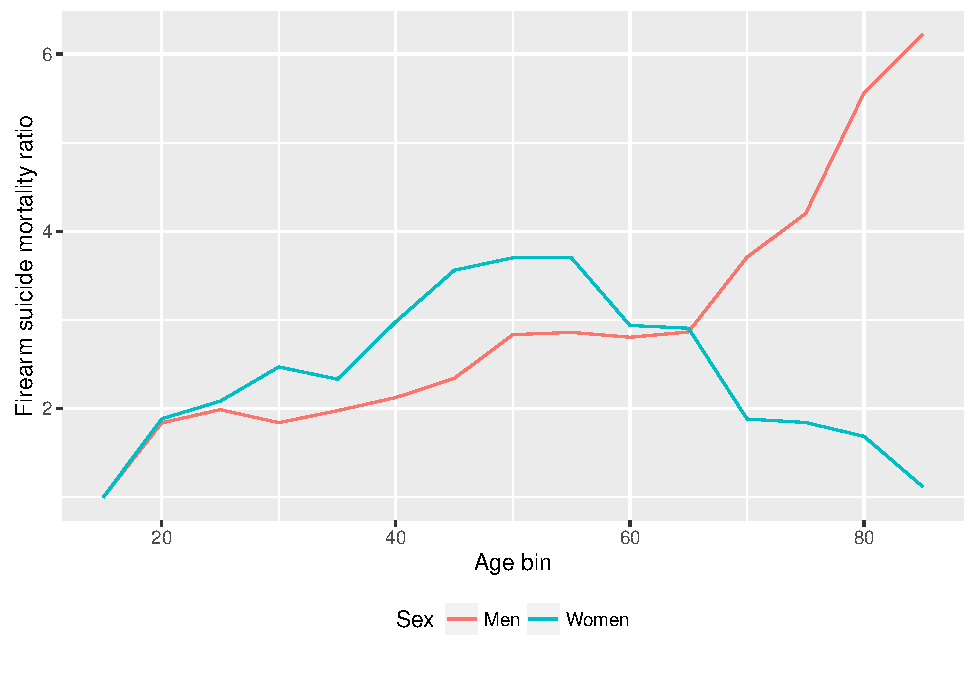
\includegraphics{Thesis_files/figure-latex/age-plot-1.pdf}
\caption{Ratio of firearm suicide mortality in age bin \(x\) to age bin
15 in 2013 by sex}
\end{figure}

Over time, the rate of suicide (both aggregated and by means) is
relatively constant within men and women. Specifically, firearm suicide
mortality rates decreased by an average of 0.02 deaths per 100,000
people in men and 0.01 deaths per 100,000 people in women annually
between 1980 and 2013. In 2013, the five states with the highest firearm
suicide mortality rates were (in order) Alaska, Wyoming, Montana, Idaho,
and West Virginia, and the states with highest overall suicide mortality
rate were Alaska, Montana, Wyoming, Utah, and New Mexico.

The list of IHME unified counties contains 3,109 counties. With 15 age
groups (15-19, 20-24,\ldots{}85+), two sexes, and 34 years, our final
dataset contained 3,171,180 observations. Of these, 2,803,876 had zero
firearm suicide deaths and 2,902,802 had zero suicide deaths by other
means. As we can see in Figure 3, this led to a heavily zero-inflated
distrubtion of firerm suicide mortality rates in 2013.

\begin{figure}[htbp]
\centering
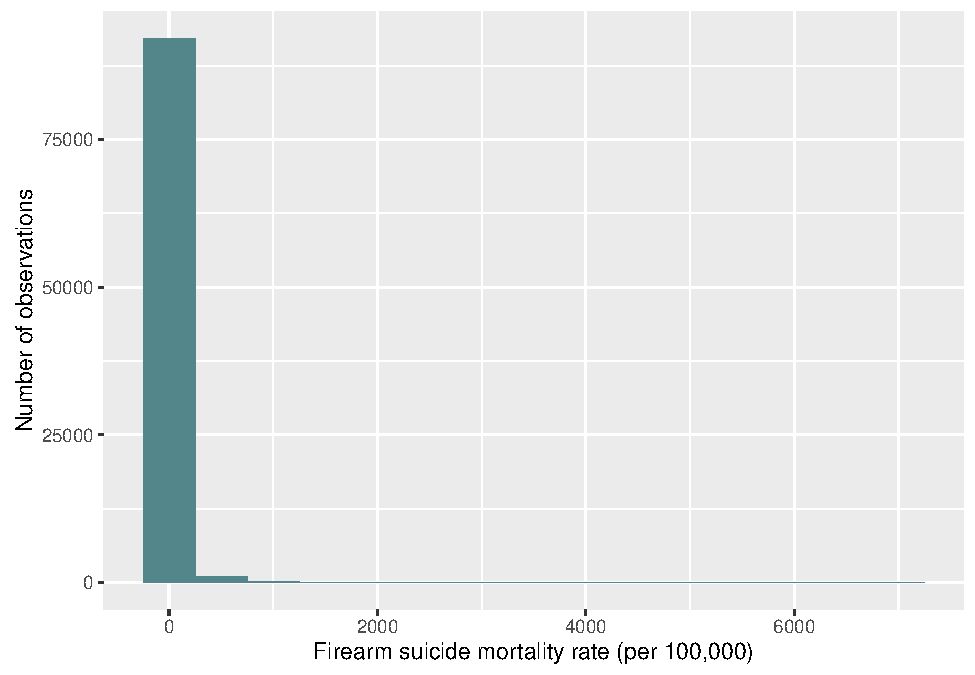
\includegraphics{Thesis_files/figure-latex/zero-hist-1.pdf}
\caption{Distribution of firearm mortality rates across counties in
2013}
\end{figure}

\subsection{Exposure Variables}\label{exposure-variables}

We identified 13 states with PTP requirements in 2013 (California,
Connecticut, Hawaii, Illinois, Iowa, Massachusetts, Michigan, Minnesota,
Nebraska, New Jersey, New York, North Carolina, and Rhode Island). 14
states had a PTP requirement at any point during the study period,
leading to 417 state-years of any level of exposure. The earliest PTP
requirement we were able to identify was passed by Massachusetts in
1906, and the most recent was passed by Maryland in 2013. We were not
able to identify any laws passed and repealed before 1995, so the
original search strategy seems to have been comprehensive. Missouri
repealed its PTP requirement in 2007 and was the only state to do so
during the study period.

There was considerable variation in the actual content of the PTP
requirements, which we did not consider in this study. For instance,
Illinois requires all potential handgun purchasers to have a valid
Firearm Owners Identification card. The card is valid for 5 years, and
the licensed individual can purchase as many handguns as they desire
over that period. This contrasts with Michigan, which requires a
short-term, 10-day license for every new handgun purchase. It seems
likely that these laws vary in their relative effectiveness, but our
models had no way to account that.

\subsection{Estimates}\label{estimates}

\subsubsection{Main Analysis}\label{main-analysis}

We present results from the three models of our main analysis in Table
1, which contains linear coefficients and standard errors associated
with those coefficients. One, two, and three asterisks indicate
significance at the 0.05, 0.01, and 0.001 levels respectively. We
restricted the exposure indicators reported in Table 1 for the sake of
conciseness; we included the first five years and 10 years, 20 years,
and 35 years of policy-time in the table. Additionally, we only included
age bins 10 years apart. Full results are presented in Appendix Table 4.
All plots of effect estimates are relative risks (exponentiated linear
coefficients).

\begin{longtable}[c]{@{}rrrrrrr@{}}
\caption{Results of Poisson regressions with firearm suicide as
dependent variable. Point estimates are coefficients from linear model.
Standard errors are presented in parentheses. One, two, and three
asterisks indicate significance at the 0.05, 0.01, and 0.001 levels
respectively.}\tabularnewline
\toprule
\begin{minipage}[b]{0.12\columnwidth}\raggedleft\strut
Variable
\strut\end{minipage} &
\begin{minipage}[b]{0.11\columnwidth}\raggedleft\strut
Model 1
\strut\end{minipage} &
\begin{minipage}[b]{0.12\columnwidth}\raggedleft\strut
~
\strut\end{minipage} &
\begin{minipage}[b]{0.11\columnwidth}\raggedleft\strut
Model 2
\strut\end{minipage} &
\begin{minipage}[b]{0.12\columnwidth}\raggedleft\strut
~
\strut\end{minipage} &
\begin{minipage}[b]{0.11\columnwidth}\raggedleft\strut
Model 3
\strut\end{minipage} &
\begin{minipage}[b]{0.11\columnwidth}\raggedleft\strut
~
\strut\end{minipage}\tabularnewline
\midrule
\endfirsthead
\toprule
\begin{minipage}[b]{0.12\columnwidth}\raggedleft\strut
Variable
\strut\end{minipage} &
\begin{minipage}[b]{0.11\columnwidth}\raggedleft\strut
Model 1
\strut\end{minipage} &
\begin{minipage}[b]{0.12\columnwidth}\raggedleft\strut
~
\strut\end{minipage} &
\begin{minipage}[b]{0.11\columnwidth}\raggedleft\strut
Model 2
\strut\end{minipage} &
\begin{minipage}[b]{0.12\columnwidth}\raggedleft\strut
~
\strut\end{minipage} &
\begin{minipage}[b]{0.11\columnwidth}\raggedleft\strut
Model 3
\strut\end{minipage} &
\begin{minipage}[b]{0.11\columnwidth}\raggedleft\strut
~
\strut\end{minipage}\tabularnewline
\midrule
\endhead
\begin{minipage}[t]{0.12\columnwidth}\raggedleft\strut
\strut\end{minipage} &
\begin{minipage}[t]{0.11\columnwidth}\raggedleft\strut
\textbf{Men}
\strut\end{minipage} &
\begin{minipage}[t]{0.12\columnwidth}\raggedleft\strut
\textbf{Women}
\strut\end{minipage} &
\begin{minipage}[t]{0.11\columnwidth}\raggedleft\strut
\textbf{Men}
\strut\end{minipage} &
\begin{minipage}[t]{0.12\columnwidth}\raggedleft\strut
\textbf{Women}
\strut\end{minipage} &
\begin{minipage}[t]{0.11\columnwidth}\raggedleft\strut
\textbf{Men}
\strut\end{minipage} &
\begin{minipage}[t]{0.11\columnwidth}\raggedleft\strut
\textbf{Women}
\strut\end{minipage}\tabularnewline
\begin{minipage}[t]{0.12\columnwidth}\raggedleft\strut
Intercept
\strut\end{minipage} &
\begin{minipage}[t]{0.11\columnwidth}\raggedleft\strut
-8.48*** (0.043)
\strut\end{minipage} &
\begin{minipage}[t]{0.12\columnwidth}\raggedleft\strut
-10.51*** (0.067)
\strut\end{minipage} &
\begin{minipage}[t]{0.11\columnwidth}\raggedleft\strut
-8.97*** (0.048)
\strut\end{minipage} &
\begin{minipage}[t]{0.12\columnwidth}\raggedleft\strut
-10.87*** (0.073)
\strut\end{minipage} &
\begin{minipage}[t]{0.11\columnwidth}\raggedleft\strut
-8.64*** (0.035)
\strut\end{minipage} &
\begin{minipage}[t]{0.11\columnwidth}\raggedleft\strut
-10.65*** (0.067)
\strut\end{minipage}\tabularnewline
\begin{minipage}[t]{0.12\columnwidth}\raggedleft\strut
Scaled year
\strut\end{minipage} &
\begin{minipage}[t]{0.11\columnwidth}\raggedleft\strut
-
\strut\end{minipage} &
\begin{minipage}[t]{0.12\columnwidth}\raggedleft\strut
-
\strut\end{minipage} &
\begin{minipage}[t]{0.11\columnwidth}\raggedleft\strut
-0.29*** (0.005)
\strut\end{minipage} &
\begin{minipage}[t]{0.12\columnwidth}\raggedleft\strut
-0.49*** (0.013)
\strut\end{minipage} &
\begin{minipage}[t]{0.11\columnwidth}\raggedleft\strut
-0.15*** (0.008)
\strut\end{minipage} &
\begin{minipage}[t]{0.11\columnwidth}\raggedleft\strut
-0.37*** (0.017)
\strut\end{minipage}\tabularnewline
\begin{minipage}[t]{0.12\columnwidth}\raggedleft\strut
Population density
\strut\end{minipage} &
\begin{minipage}[t]{0.11\columnwidth}\raggedleft\strut
-
\strut\end{minipage} &
\begin{minipage}[t]{0.12\columnwidth}\raggedleft\strut
-
\strut\end{minipage} &
\begin{minipage}[t]{0.11\columnwidth}\raggedleft\strut
-
\strut\end{minipage} &
\begin{minipage}[t]{0.12\columnwidth}\raggedleft\strut
-
\strut\end{minipage} &
\begin{minipage}[t]{0.11\columnwidth}\raggedleft\strut
-0.08*** (0.004)
\strut\end{minipage} &
\begin{minipage}[t]{0.11\columnwidth}\raggedleft\strut
-0.05*** (0.006)
\strut\end{minipage}\tabularnewline
\begin{minipage}[t]{0.12\columnwidth}\raggedleft\strut
Unemployement
\strut\end{minipage} &
\begin{minipage}[t]{0.11\columnwidth}\raggedleft\strut
-
\strut\end{minipage} &
\begin{minipage}[t]{0.12\columnwidth}\raggedleft\strut
-
\strut\end{minipage} &
\begin{minipage}[t]{0.11\columnwidth}\raggedleft\strut
-
\strut\end{minipage} &
\begin{minipage}[t]{0.12\columnwidth}\raggedleft\strut
-
\strut\end{minipage} &
\begin{minipage}[t]{0.11\columnwidth}\raggedleft\strut
0.80*** (0.081)
\strut\end{minipage} &
\begin{minipage}[t]{0.11\columnwidth}\raggedleft\strut
1.03*** (0.195)
\strut\end{minipage}\tabularnewline
\begin{minipage}[t]{0.12\columnwidth}\raggedleft\strut
College education
\strut\end{minipage} &
\begin{minipage}[t]{0.11\columnwidth}\raggedleft\strut
-
\strut\end{minipage} &
\begin{minipage}[t]{0.12\columnwidth}\raggedleft\strut
-
\strut\end{minipage} &
\begin{minipage}[t]{0.11\columnwidth}\raggedleft\strut
-
\strut\end{minipage} &
\begin{minipage}[t]{0.12\columnwidth}\raggedleft\strut
-
\strut\end{minipage} &
\begin{minipage}[t]{0.11\columnwidth}\raggedleft\strut
-1.10*** (0.061)
\strut\end{minipage} &
\begin{minipage}[t]{0.11\columnwidth}\raggedleft\strut
-0.83*** (0.118)
\strut\end{minipage}\tabularnewline
\begin{minipage}[t]{0.12\columnwidth}\raggedleft\strut
Income
\strut\end{minipage} &
\begin{minipage}[t]{0.11\columnwidth}\raggedleft\strut
-
\strut\end{minipage} &
\begin{minipage}[t]{0.12\columnwidth}\raggedleft\strut
-
\strut\end{minipage} &
\begin{minipage}[t]{0.11\columnwidth}\raggedleft\strut
-
\strut\end{minipage} &
\begin{minipage}[t]{0.12\columnwidth}\raggedleft\strut
-
\strut\end{minipage} &
\begin{minipage}[t]{0.11\columnwidth}\raggedleft\strut
0.01 (0.004)
\strut\end{minipage} &
\begin{minipage}[t]{0.11\columnwidth}\raggedleft\strut
-0.02* (0.009)
\strut\end{minipage}\tabularnewline
\begin{minipage}[t]{0.12\columnwidth}\raggedleft\strut
Age 20
\strut\end{minipage} &
\begin{minipage}[t]{0.11\columnwidth}\raggedleft\strut
-
\strut\end{minipage} &
\begin{minipage}[t]{0.12\columnwidth}\raggedleft\strut
-
\strut\end{minipage} &
\begin{minipage}[t]{0.11\columnwidth}\raggedleft\strut
0.51*** (0.007)
\strut\end{minipage} &
\begin{minipage}[t]{0.12\columnwidth}\raggedleft\strut
0.33*** (0.020)
\strut\end{minipage} &
\begin{minipage}[t]{0.11\columnwidth}\raggedleft\strut
0.51*** (0.007)
\strut\end{minipage} &
\begin{minipage}[t]{0.11\columnwidth}\raggedleft\strut
0.33*** (0.020)
\strut\end{minipage}\tabularnewline
\begin{minipage}[t]{0.12\columnwidth}\raggedleft\strut
Age 30
\strut\end{minipage} &
\begin{minipage}[t]{0.11\columnwidth}\raggedleft\strut
-
\strut\end{minipage} &
\begin{minipage}[t]{0.12\columnwidth}\raggedleft\strut
-
\strut\end{minipage} &
\begin{minipage}[t]{0.11\columnwidth}\raggedleft\strut
0.37*** (0.008)
\strut\end{minipage} &
\begin{minipage}[t]{0.12\columnwidth}\raggedleft\strut
0.52*** (0.019)
\strut\end{minipage} &
\begin{minipage}[t]{0.11\columnwidth}\raggedleft\strut
0.37*** (0.008)
\strut\end{minipage} &
\begin{minipage}[t]{0.11\columnwidth}\raggedleft\strut
0.52*** (0.019)
\strut\end{minipage}\tabularnewline
\begin{minipage}[t]{0.12\columnwidth}\raggedleft\strut
Age 40
\strut\end{minipage} &
\begin{minipage}[t]{0.11\columnwidth}\raggedleft\strut
-
\strut\end{minipage} &
\begin{minipage}[t]{0.12\columnwidth}\raggedleft\strut
-
\strut\end{minipage} &
\begin{minipage}[t]{0.11\columnwidth}\raggedleft\strut
0.42*** (0.008)
\strut\end{minipage} &
\begin{minipage}[t]{0.12\columnwidth}\raggedleft\strut
0.71*** (0.019)
\strut\end{minipage} &
\begin{minipage}[t]{0.11\columnwidth}\raggedleft\strut
0.42*** (0.008)
\strut\end{minipage} &
\begin{minipage}[t]{0.11\columnwidth}\raggedleft\strut
0.72*** (0.019)
\strut\end{minipage}\tabularnewline
\begin{minipage}[t]{0.12\columnwidth}\raggedleft\strut
Age 50
\strut\end{minipage} &
\begin{minipage}[t]{0.11\columnwidth}\raggedleft\strut
-
\strut\end{minipage} &
\begin{minipage}[t]{0.12\columnwidth}\raggedleft\strut
-
\strut\end{minipage} &
\begin{minipage}[t]{0.11\columnwidth}\raggedleft\strut
0.59*** (0.008)
\strut\end{minipage} &
\begin{minipage}[t]{0.12\columnwidth}\raggedleft\strut
0.80*** (0.019)
\strut\end{minipage} &
\begin{minipage}[t]{0.11\columnwidth}\raggedleft\strut
0.59*** (0.008)
\strut\end{minipage} &
\begin{minipage}[t]{0.11\columnwidth}\raggedleft\strut
0.80*** (0.019)
\strut\end{minipage}\tabularnewline
\begin{minipage}[t]{0.12\columnwidth}\raggedleft\strut
Age 60
\strut\end{minipage} &
\begin{minipage}[t]{0.11\columnwidth}\raggedleft\strut
-
\strut\end{minipage} &
\begin{minipage}[t]{0.12\columnwidth}\raggedleft\strut
-
\strut\end{minipage} &
\begin{minipage}[t]{0.11\columnwidth}\raggedleft\strut
0.66*** (0.008)
\strut\end{minipage} &
\begin{minipage}[t]{0.12\columnwidth}\raggedleft\strut
0.60*** (0.021)
\strut\end{minipage} &
\begin{minipage}[t]{0.11\columnwidth}\raggedleft\strut
0.66*** (0.008)
\strut\end{minipage} &
\begin{minipage}[t]{0.11\columnwidth}\raggedleft\strut
0.60*** (0.021)
\strut\end{minipage}\tabularnewline
\begin{minipage}[t]{0.12\columnwidth}\raggedleft\strut
Age 70
\strut\end{minipage} &
\begin{minipage}[t]{0.11\columnwidth}\raggedleft\strut
-
\strut\end{minipage} &
\begin{minipage}[t]{0.12\columnwidth}\raggedleft\strut
-
\strut\end{minipage} &
\begin{minipage}[t]{0.11\columnwidth}\raggedleft\strut
1.01*** (0.008)
\strut\end{minipage} &
\begin{minipage}[t]{0.12\columnwidth}\raggedleft\strut
0.35*** (0.024)
\strut\end{minipage} &
\begin{minipage}[t]{0.11\columnwidth}\raggedleft\strut
1.01*** (0.008)
\strut\end{minipage} &
\begin{minipage}[t]{0.11\columnwidth}\raggedleft\strut
0.35*** (0.024)
\strut\end{minipage}\tabularnewline
\begin{minipage}[t]{0.12\columnwidth}\raggedleft\strut
Age 80
\strut\end{minipage} &
\begin{minipage}[t]{0.11\columnwidth}\raggedleft\strut
-
\strut\end{minipage} &
\begin{minipage}[t]{0.12\columnwidth}\raggedleft\strut
-
\strut\end{minipage} &
\begin{minipage}[t]{0.11\columnwidth}\raggedleft\strut
1.47*** (0.009)
\strut\end{minipage} &
\begin{minipage}[t]{0.12\columnwidth}\raggedleft\strut
0.08* (0.031)
\strut\end{minipage} &
\begin{minipage}[t]{0.11\columnwidth}\raggedleft\strut
1.46*** (0.009)
\strut\end{minipage} &
\begin{minipage}[t]{0.11\columnwidth}\raggedleft\strut
0.08* (0.031)
\strut\end{minipage}\tabularnewline
\begin{minipage}[t]{0.12\columnwidth}\raggedleft\strut
PTP year 1
\strut\end{minipage} &
\begin{minipage}[t]{0.11\columnwidth}\raggedleft\strut
-0.15*** (0.022)
\strut\end{minipage} &
\begin{minipage}[t]{0.12\columnwidth}\raggedleft\strut
-0.23*** (0.055)
\strut\end{minipage} &
\begin{minipage}[t]{0.11\columnwidth}\raggedleft\strut
-0.13*** (0.022)
\strut\end{minipage} &
\begin{minipage}[t]{0.12\columnwidth}\raggedleft\strut
-0.19*** (0.055)
\strut\end{minipage} &
\begin{minipage}[t]{0.11\columnwidth}\raggedleft\strut
-0.13*** (0.022)
\strut\end{minipage} &
\begin{minipage}[t]{0.11\columnwidth}\raggedleft\strut
-0.20*** (0.055)
\strut\end{minipage}\tabularnewline
\begin{minipage}[t]{0.12\columnwidth}\raggedleft\strut
PTP year 2
\strut\end{minipage} &
\begin{minipage}[t]{0.11\columnwidth}\raggedleft\strut
-0.21*** (0.021)
\strut\end{minipage} &
\begin{minipage}[t]{0.12\columnwidth}\raggedleft\strut
-0.42*** (0.058)
\strut\end{minipage} &
\begin{minipage}[t]{0.11\columnwidth}\raggedleft\strut
-0.18*** (0.021)
\strut\end{minipage} &
\begin{minipage}[t]{0.12\columnwidth}\raggedleft\strut
-0.36*** (0.058)
\strut\end{minipage} &
\begin{minipage}[t]{0.11\columnwidth}\raggedleft\strut
-0.17*** (0.021)
\strut\end{minipage} &
\begin{minipage}[t]{0.11\columnwidth}\raggedleft\strut
-0.36*** (0.058)
\strut\end{minipage}\tabularnewline
\begin{minipage}[t]{0.12\columnwidth}\raggedleft\strut
PTP year 3
\strut\end{minipage} &
\begin{minipage}[t]{0.11\columnwidth}\raggedleft\strut
-0.26*** (0.021)
\strut\end{minipage} &
\begin{minipage}[t]{0.12\columnwidth}\raggedleft\strut
-0.33*** (0.053)
\strut\end{minipage} &
\begin{minipage}[t]{0.11\columnwidth}\raggedleft\strut
-0.22*** (0.021)
\strut\end{minipage} &
\begin{minipage}[t]{0.12\columnwidth}\raggedleft\strut
-0.26*** (0.053)
\strut\end{minipage} &
\begin{minipage}[t]{0.11\columnwidth}\raggedleft\strut
-0.21*** (0.021)
\strut\end{minipage} &
\begin{minipage}[t]{0.11\columnwidth}\raggedleft\strut
-0.26*** (0.053)
\strut\end{minipage}\tabularnewline
\begin{minipage}[t]{0.12\columnwidth}\raggedleft\strut
PTP year 4
\strut\end{minipage} &
\begin{minipage}[t]{0.11\columnwidth}\raggedleft\strut
-0.27*** (0.021)
\strut\end{minipage} &
\begin{minipage}[t]{0.12\columnwidth}\raggedleft\strut
-0.42*** (0.055)
\strut\end{minipage} &
\begin{minipage}[t]{0.11\columnwidth}\raggedleft\strut
-0.23*** (0.021)
\strut\end{minipage} &
\begin{minipage}[t]{0.12\columnwidth}\raggedleft\strut
-0.34*** (0.055)
\strut\end{minipage} &
\begin{minipage}[t]{0.11\columnwidth}\raggedleft\strut
-0.22*** (0.021)
\strut\end{minipage} &
\begin{minipage}[t]{0.11\columnwidth}\raggedleft\strut
-0.33*** (0.055)
\strut\end{minipage}\tabularnewline
\begin{minipage}[t]{0.12\columnwidth}\raggedleft\strut
PTP year 5
\strut\end{minipage} &
\begin{minipage}[t]{0.11\columnwidth}\raggedleft\strut
-0.31*** (0.021)
\strut\end{minipage} &
\begin{minipage}[t]{0.12\columnwidth}\raggedleft\strut
-0.54*** (0.058)
\strut\end{minipage} &
\begin{minipage}[t]{0.11\columnwidth}\raggedleft\strut
-0.26*** (0.021)
\strut\end{minipage} &
\begin{minipage}[t]{0.12\columnwidth}\raggedleft\strut
-0.45*** (0.058)
\strut\end{minipage} &
\begin{minipage}[t]{0.11\columnwidth}\raggedleft\strut
-0.25*** (0.021)
\strut\end{minipage} &
\begin{minipage}[t]{0.11\columnwidth}\raggedleft\strut
-0.43*** (0.058)
\strut\end{minipage}\tabularnewline
\begin{minipage}[t]{0.12\columnwidth}\raggedleft\strut
PTP year 10
\strut\end{minipage} &
\begin{minipage}[t]{0.11\columnwidth}\raggedleft\strut
-0.42*** (0.021)
\strut\end{minipage} &
\begin{minipage}[t]{0.12\columnwidth}\raggedleft\strut
-0.71*** (0.061)
\strut\end{minipage} &
\begin{minipage}[t]{0.11\columnwidth}\raggedleft\strut
-0.33*** (0.022)
\strut\end{minipage} &
\begin{minipage}[t]{0.12\columnwidth}\raggedleft\strut
-0.55*** (0.061)
\strut\end{minipage} &
\begin{minipage}[t]{0.11\columnwidth}\raggedleft\strut
-0.32*** (0.022)
\strut\end{minipage} &
\begin{minipage}[t]{0.11\columnwidth}\raggedleft\strut
-0.53*** (0.061)
\strut\end{minipage}\tabularnewline
\begin{minipage}[t]{0.12\columnwidth}\raggedleft\strut
PTP year 20
\strut\end{minipage} &
\begin{minipage}[t]{0.11\columnwidth}\raggedleft\strut
-0.40*** (0.024)
\strut\end{minipage} &
\begin{minipage}[t]{0.12\columnwidth}\raggedleft\strut
-0.65*** (0.072)
\strut\end{minipage} &
\begin{minipage}[t]{0.11\columnwidth}\raggedleft\strut
-0.25*** (0.025)
\strut\end{minipage} &
\begin{minipage}[t]{0.12\columnwidth}\raggedleft\strut
-0.40*** (0.072)
\strut\end{minipage} &
\begin{minipage}[t]{0.11\columnwidth}\raggedleft\strut
-0.24*** (0.025)
\strut\end{minipage} &
\begin{minipage}[t]{0.11\columnwidth}\raggedleft\strut
-0.37*** (0.072)
\strut\end{minipage}\tabularnewline
\begin{minipage}[t]{0.12\columnwidth}\raggedleft\strut
PTP year 35
\strut\end{minipage} &
\begin{minipage}[t]{0.11\columnwidth}\raggedleft\strut
-0.66*** (0.015)
\strut\end{minipage} &
\begin{minipage}[t]{0.12\columnwidth}\raggedleft\strut
-1.13*** (0.046)
\strut\end{minipage} &
\begin{minipage}[t]{0.11\columnwidth}\raggedleft\strut
-0.37*** (0.017)
\strut\end{minipage} &
\begin{minipage}[t]{0.12\columnwidth}\raggedleft\strut
-0.59*** (0.049)
\strut\end{minipage} &
\begin{minipage}[t]{0.11\columnwidth}\raggedleft\strut
-0.35*** (0.017)
\strut\end{minipage} &
\begin{minipage}[t]{0.11\columnwidth}\raggedleft\strut
-0.56*** (0.049)
\strut\end{minipage}\tabularnewline
\begin{minipage}[t]{0.12\columnwidth}\raggedleft\strut
Log-likelihood
\strut\end{minipage} &
\begin{minipage}[t]{0.11\columnwidth}\raggedleft\strut
-853,256
\strut\end{minipage} &
\begin{minipage}[t]{0.12\columnwidth}\raggedleft\strut
-237,297
\strut\end{minipage} &
\begin{minipage}[t]{0.11\columnwidth}\raggedleft\strut
-823,432
\strut\end{minipage} &
\begin{minipage}[t]{0.12\columnwidth}\raggedleft\strut
-234,225
\strut\end{minipage} &
\begin{minipage}[t]{0.11\columnwidth}\raggedleft\strut
-822,643
\strut\end{minipage} &
\begin{minipage}[t]{0.11\columnwidth}\raggedleft\strut
-234,015
\strut\end{minipage}\tabularnewline
\bottomrule
\end{longtable}

The baseline model (Model 1) showed a strong protective association
between years since PTP requirement passage and firearm suicide
mortality for both men and women. The effect increased through years 1
through 10 and gradually plateaued through year 35. Every year was
significant at our prespecified alpha level. The effect was stronger but
less precise in women than in men.

The structural model (Model 2), which added age bin indicator variables
and year, showed a similar significant association between PTP
requirement duration and firearm suicide mortality. The effect increases
over approximately the first 10 years and then begins to decrease or
plateau. The coefficient on year captures a slow decline in firearm
suicide mortality that is similar between men and women. The importance
of running separate models for men and women is illustrated by the
radically different age patterns of the coefficients for men and women.
Among men, the effect of age relative to the 15-19 age bin was uniformly
positive, decreasing slightly in magnitude until age bin 35-39 and then
increasing rapidly through age bin 85+. Among women, the pattern was
reversed; we observed a positive coefficient that increased in magnitude
until age bin 50-54 and then decreased until age bin 85+, at which point
it became negative.

In the full model (Model 3), we observed similar effects in both men and
women. Of the additional variables (log-transformed population density,
unemployment, share of the population a bachlor's degree or higher, and
z-scores of income), population density and education were protective
and significant in both men and women. Unemployment was a significant
risk factor for both men and women. Income was an insignificant risk
factor in men and significantly protective in women. We observed that
the effects of time since PTP passage were extremely similar to those we
observed in the previous two models. In both men and women, the
protective effect of PTP increased for 10 years and decreased or
plateaued after that. Figure 4 shows the relative risk esimates
associated with each time-since-passage. For men and women, the initial
decreases in relative risk bottom out at 0.708 (95\% CI: 0.679-0.739)
and 0.532 (95\% CI: 0.469-0.605) after 11 and 12 years respectively.

\begin{figure}[htbp]
\centering
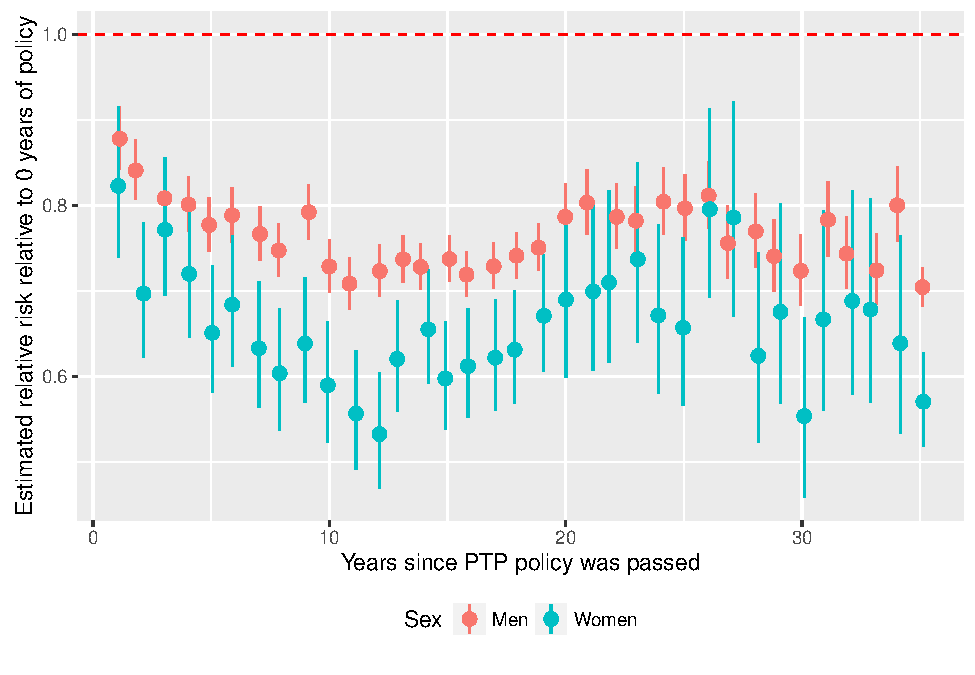
\includegraphics{Thesis_files/figure-latex/RR-plot-1.pdf}
\caption{Estimated relative risk of firearm suicide death by years since
PTP passage for men and women. Point estimates are circles and 95\%
confidence intervals are line ranges.}
\end{figure}

\subsubsection{Secondary Analysis}\label{secondary-analysis}

Table 2 presents the results of running the full model from the main
analysis with non-firearm suicide deaths and all suicide deaths as the
dependent variables. Contrary to the theory that restricting access to
firearms will increase suicide mortality by other means, we found that
PTP requirements had actually a significant protective effect that
increased with the duration of the requirement. The effects were smaller
than the effects for the main analysis, but this result was still
surprising. We plotted the full set of relative risks from the
regression on non-firearm suicide in Figure 5.

\begin{longtable}[c]{@{}rrrrr@{}}
\caption{Results of secondary analyses. Point estimates are coefficients
from linear model. Standard errors are presented in parentheses. One,
two, and three asterisks indicate significance at the 0.05, 0.01, and
0.001 levels respectively.}\tabularnewline
\toprule
\begin{minipage}[b]{0.17\columnwidth}\raggedleft\strut
Variable
\strut\end{minipage} &
\begin{minipage}[b]{0.20\columnwidth}\raggedleft\strut
Other suicide deaths
\strut\end{minipage} &
\begin{minipage}[b]{0.16\columnwidth}\raggedleft\strut
~
\strut\end{minipage} &
\begin{minipage}[b]{0.18\columnwidth}\raggedleft\strut
All suicide deaths
\strut\end{minipage} &
\begin{minipage}[b]{0.15\columnwidth}\raggedleft\strut
~
\strut\end{minipage}\tabularnewline
\midrule
\endfirsthead
\toprule
\begin{minipage}[b]{0.17\columnwidth}\raggedleft\strut
Variable
\strut\end{minipage} &
\begin{minipage}[b]{0.20\columnwidth}\raggedleft\strut
Other suicide deaths
\strut\end{minipage} &
\begin{minipage}[b]{0.16\columnwidth}\raggedleft\strut
~
\strut\end{minipage} &
\begin{minipage}[b]{0.18\columnwidth}\raggedleft\strut
All suicide deaths
\strut\end{minipage} &
\begin{minipage}[b]{0.15\columnwidth}\raggedleft\strut
~
\strut\end{minipage}\tabularnewline
\midrule
\endhead
\begin{minipage}[t]{0.17\columnwidth}\raggedleft\strut
\strut\end{minipage} &
\begin{minipage}[t]{0.20\columnwidth}\raggedleft\strut
\textbf{Men}
\strut\end{minipage} &
\begin{minipage}[t]{0.16\columnwidth}\raggedleft\strut
\textbf{Women}
\strut\end{minipage} &
\begin{minipage}[t]{0.18\columnwidth}\raggedleft\strut
\textbf{Men}
\strut\end{minipage} &
\begin{minipage}[t]{0.15\columnwidth}\raggedleft\strut
\textbf{Women}
\strut\end{minipage}\tabularnewline
\begin{minipage}[t]{0.17\columnwidth}\raggedleft\strut
Intercept
\strut\end{minipage} &
\begin{minipage}[t]{0.20\columnwidth}\raggedleft\strut
-10.16*** (0.051)
\strut\end{minipage} &
\begin{minipage}[t]{0.16\columnwidth}\raggedleft\strut
-11.36*** (0.058)
\strut\end{minipage} &
\begin{minipage}[t]{0.18\columnwidth}\raggedleft\strut
-8.50*** (0.026)
\strut\end{minipage} &
\begin{minipage}[t]{0.15\columnwidth}\raggedleft\strut
-10.38*** (0.039)
\strut\end{minipage}\tabularnewline
\begin{minipage}[t]{0.17\columnwidth}\raggedleft\strut
Scaled year
\strut\end{minipage} &
\begin{minipage}[t]{0.20\columnwidth}\raggedleft\strut
0.37*** (0.011)
\strut\end{minipage} &
\begin{minipage}[t]{0.16\columnwidth}\raggedleft\strut
0.05** (0.016)
\strut\end{minipage} &
\begin{minipage}[t]{0.18\columnwidth}\raggedleft\strut
0.02* (0.007)
\strut\end{minipage} &
\begin{minipage}[t]{0.15\columnwidth}\raggedleft\strut
-0.15*** (0.012)
\strut\end{minipage}\tabularnewline
\begin{minipage}[t]{0.17\columnwidth}\raggedleft\strut
Population density
\strut\end{minipage} &
\begin{minipage}[t]{0.20\columnwidth}\raggedleft\strut
0.10*** (0.005)
\strut\end{minipage} &
\begin{minipage}[t]{0.16\columnwidth}\raggedleft\strut
0.11*** (0.006)
\strut\end{minipage} &
\begin{minipage}[t]{0.18\columnwidth}\raggedleft\strut
-0.03*** (0.003)
\strut\end{minipage} &
\begin{minipage}[t]{0.15\columnwidth}\raggedleft\strut
0.04*** (0.005)
\strut\end{minipage}\tabularnewline
\begin{minipage}[t]{0.17\columnwidth}\raggedleft\strut
Unemployement
\strut\end{minipage} &
\begin{minipage}[t]{0.20\columnwidth}\raggedleft\strut
1.11*** (0.104)
\strut\end{minipage} &
\begin{minipage}[t]{0.16\columnwidth}\raggedleft\strut
1.82*** (0.157)
\strut\end{minipage} &
\begin{minipage}[t]{0.18\columnwidth}\raggedleft\strut
1.03*** (0.064)
\strut\end{minipage} &
\begin{minipage}[t]{0.15\columnwidth}\raggedleft\strut
1.66*** (0.123)
\strut\end{minipage}\tabularnewline
\begin{minipage}[t]{0.17\columnwidth}\raggedleft\strut
College education
\strut\end{minipage} &
\begin{minipage}[t]{0.20\columnwidth}\raggedleft\strut
-1.01*** (0.077)
\strut\end{minipage} &
\begin{minipage}[t]{0.16\columnwidth}\raggedleft\strut
0.14 (0.104)
\strut\end{minipage} &
\begin{minipage}[t]{0.18\columnwidth}\raggedleft\strut
-0.82*** (0.050)
\strut\end{minipage} &
\begin{minipage}[t]{0.15\columnwidth}\raggedleft\strut
0.00 (0.082)
\strut\end{minipage}\tabularnewline
\begin{minipage}[t]{0.17\columnwidth}\raggedleft\strut
Income
\strut\end{minipage} &
\begin{minipage}[t]{0.20\columnwidth}\raggedleft\strut
-0.03*** (0.005)
\strut\end{minipage} &
\begin{minipage}[t]{0.16\columnwidth}\raggedleft\strut
-0.04*** (0.007)
\strut\end{minipage} &
\begin{minipage}[t]{0.18\columnwidth}\raggedleft\strut
-0.01** (0.003)
\strut\end{minipage} &
\begin{minipage}[t]{0.15\columnwidth}\raggedleft\strut
-0.04*** (0.006)
\strut\end{minipage}\tabularnewline
\begin{minipage}[t]{0.17\columnwidth}\raggedleft\strut
Age 20
\strut\end{minipage} &
\begin{minipage}[t]{0.20\columnwidth}\raggedleft\strut
0.54*** (0.009)
\strut\end{minipage} &
\begin{minipage}[t]{0.16\columnwidth}\raggedleft\strut
0.19*** (0.017)
\strut\end{minipage} &
\begin{minipage}[t]{0.18\columnwidth}\raggedleft\strut
0.52*** (0.006)
\strut\end{minipage} &
\begin{minipage}[t]{0.15\columnwidth}\raggedleft\strut
0.25*** (0.013)
\strut\end{minipage}\tabularnewline
\begin{minipage}[t]{0.17\columnwidth}\raggedleft\strut
Age 30
\strut\end{minipage} &
\begin{minipage}[t]{0.20\columnwidth}\raggedleft\strut
0.65*** (0.009)
\strut\end{minipage} &
\begin{minipage}[t]{0.16\columnwidth}\raggedleft\strut
0.57*** (0.015)
\strut\end{minipage} &
\begin{minipage}[t]{0.18\columnwidth}\raggedleft\strut
0.49*** (0.006)
\strut\end{minipage} &
\begin{minipage}[t]{0.15\columnwidth}\raggedleft\strut
0.55*** (0.012)
\strut\end{minipage}\tabularnewline
\begin{minipage}[t]{0.17\columnwidth}\raggedleft\strut
Age 40
\strut\end{minipage} &
\begin{minipage}[t]{0.20\columnwidth}\raggedleft\strut
0.69*** (0.009)
\strut\end{minipage} &
\begin{minipage}[t]{0.16\columnwidth}\raggedleft\strut
0.91*** (0.015)
\strut\end{minipage} &
\begin{minipage}[t]{0.18\columnwidth}\raggedleft\strut
0.54*** (0.006)
\strut\end{minipage} &
\begin{minipage}[t]{0.15\columnwidth}\raggedleft\strut
0.84*** (0.012)
\strut\end{minipage}\tabularnewline
\begin{minipage}[t]{0.17\columnwidth}\raggedleft\strut
Age 50
\strut\end{minipage} &
\begin{minipage}[t]{0.20\columnwidth}\raggedleft\strut
0.58*** (0.009)
\strut\end{minipage} &
\begin{minipage}[t]{0.16\columnwidth}\raggedleft\strut
1.00*** (0.015)
\strut\end{minipage} &
\begin{minipage}[t]{0.18\columnwidth}\raggedleft\strut
0.59*** (0.006)
\strut\end{minipage} &
\begin{minipage}[t]{0.15\columnwidth}\raggedleft\strut
0.92*** (0.012)
\strut\end{minipage}\tabularnewline
\begin{minipage}[t]{0.17\columnwidth}\raggedleft\strut
Age 60
\strut\end{minipage} &
\begin{minipage}[t]{0.20\columnwidth}\raggedleft\strut
0.23*** (0.011)
\strut\end{minipage} &
\begin{minipage}[t]{0.16\columnwidth}\raggedleft\strut
0.68*** (0.016)
\strut\end{minipage} &
\begin{minipage}[t]{0.18\columnwidth}\raggedleft\strut
0.51*** (0.007)
\strut\end{minipage} &
\begin{minipage}[t]{0.15\columnwidth}\raggedleft\strut
0.65*** (0.013)
\strut\end{minipage}\tabularnewline
\begin{minipage}[t]{0.17\columnwidth}\raggedleft\strut
Age 70
\strut\end{minipage} &
\begin{minipage}[t]{0.20\columnwidth}\raggedleft\strut
0.14*** (0.013)
\strut\end{minipage} &
\begin{minipage}[t]{0.16\columnwidth}\raggedleft\strut
0.48*** (0.019)
\strut\end{minipage} &
\begin{minipage}[t]{0.18\columnwidth}\raggedleft\strut
0.74*** (0.007)
\strut\end{minipage} &
\begin{minipage}[t]{0.15\columnwidth}\raggedleft\strut
0.43*** (0.015)
\strut\end{minipage}\tabularnewline
\begin{minipage}[t]{0.17\columnwidth}\raggedleft\strut
Age 80
\strut\end{minipage} &
\begin{minipage}[t]{0.20\columnwidth}\raggedleft\strut
0.56*** (0.015)
\strut\end{minipage} &
\begin{minipage}[t]{0.16\columnwidth}\raggedleft\strut
0.55*** (0.021)
\strut\end{minipage} &
\begin{minipage}[t]{0.18\columnwidth}\raggedleft\strut
1.18*** (0.008)
\strut\end{minipage} &
\begin{minipage}[t]{0.15\columnwidth}\raggedleft\strut
0.39*** (0.017)
\strut\end{minipage}\tabularnewline
\begin{minipage}[t]{0.17\columnwidth}\raggedleft\strut
PTP year 1
\strut\end{minipage} &
\begin{minipage}[t]{0.20\columnwidth}\raggedleft\strut
-0.07** (0.025)
\strut\end{minipage} &
\begin{minipage}[t]{0.16\columnwidth}\raggedleft\strut
-0.29*** (0.039)
\strut\end{minipage} &
\begin{minipage}[t]{0.18\columnwidth}\raggedleft\strut
-0.09*** (0.016)
\strut\end{minipage} &
\begin{minipage}[t]{0.15\columnwidth}\raggedleft\strut
-0.24*** (0.032)
\strut\end{minipage}\tabularnewline
\begin{minipage}[t]{0.17\columnwidth}\raggedleft\strut
PTP year 2
\strut\end{minipage} &
\begin{minipage}[t]{0.20\columnwidth}\raggedleft\strut
-0.16*** (0.024)
\strut\end{minipage} &
\begin{minipage}[t]{0.16\columnwidth}\raggedleft\strut
-0.24*** (0.036)
\strut\end{minipage} &
\begin{minipage}[t]{0.18\columnwidth}\raggedleft\strut
-0.16*** (0.016)
\strut\end{minipage} &
\begin{minipage}[t]{0.15\columnwidth}\raggedleft\strut
-0.26*** (0.031)
\strut\end{minipage}\tabularnewline
\begin{minipage}[t]{0.17\columnwidth}\raggedleft\strut
PTP year 3
\strut\end{minipage} &
\begin{minipage}[t]{0.20\columnwidth}\raggedleft\strut
-0.18*** (0.023)
\strut\end{minipage} &
\begin{minipage}[t]{0.16\columnwidth}\raggedleft\strut
-0.25*** (0.035)
\strut\end{minipage} &
\begin{minipage}[t]{0.18\columnwidth}\raggedleft\strut
-0.19*** (0.016)
\strut\end{minipage} &
\begin{minipage}[t]{0.15\columnwidth}\raggedleft\strut
-0.24*** (0.029)
\strut\end{minipage}\tabularnewline
\begin{minipage}[t]{0.17\columnwidth}\raggedleft\strut
PTP year 4
\strut\end{minipage} &
\begin{minipage}[t]{0.20\columnwidth}\raggedleft\strut
-0.17*** (0.023)
\strut\end{minipage} &
\begin{minipage}[t]{0.16\columnwidth}\raggedleft\strut
-0.18*** (0.034)
\strut\end{minipage} &
\begin{minipage}[t]{0.18\columnwidth}\raggedleft\strut
-0.19*** (0.015)
\strut\end{minipage} &
\begin{minipage}[t]{0.15\columnwidth}\raggedleft\strut
-0.21*** (0.029)
\strut\end{minipage}\tabularnewline
\begin{minipage}[t]{0.17\columnwidth}\raggedleft\strut
PTP year 5
\strut\end{minipage} &
\begin{minipage}[t]{0.20\columnwidth}\raggedleft\strut
-0.20*** (0.023)
\strut\end{minipage} &
\begin{minipage}[t]{0.16\columnwidth}\raggedleft\strut
-0.31*** (0.036)
\strut\end{minipage} &
\begin{minipage}[t]{0.18\columnwidth}\raggedleft\strut
-0.21*** (0.016)
\strut\end{minipage} &
\begin{minipage}[t]{0.15\columnwidth}\raggedleft\strut
-0.32*** (0.030)
\strut\end{minipage}\tabularnewline
\begin{minipage}[t]{0.17\columnwidth}\raggedleft\strut
PTP year 10
\strut\end{minipage} &
\begin{minipage}[t]{0.20\columnwidth}\raggedleft\strut
-0.17*** (0.022)
\strut\end{minipage} &
\begin{minipage}[t]{0.16\columnwidth}\raggedleft\strut
-0.21*** (0.033)
\strut\end{minipage} &
\begin{minipage}[t]{0.18\columnwidth}\raggedleft\strut
-0.22*** (0.015)
\strut\end{minipage} &
\begin{minipage}[t]{0.15\columnwidth}\raggedleft\strut
-0.26*** (0.029)
\strut\end{minipage}\tabularnewline
\begin{minipage}[t]{0.17\columnwidth}\raggedleft\strut
PTP year 20
\strut\end{minipage} &
\begin{minipage}[t]{0.20\columnwidth}\raggedleft\strut
-0.26*** (0.026)
\strut\end{minipage} &
\begin{minipage}[t]{0.16\columnwidth}\raggedleft\strut
-0.35*** (0.040)
\strut\end{minipage} &
\begin{minipage}[t]{0.18\columnwidth}\raggedleft\strut
-0.21*** (0.018)
\strut\end{minipage} &
\begin{minipage}[t]{0.15\columnwidth}\raggedleft\strut
-0.30*** (0.035)
\strut\end{minipage}\tabularnewline
\begin{minipage}[t]{0.17\columnwidth}\raggedleft\strut
PTP year 35
\strut\end{minipage} &
\begin{minipage}[t]{0.20\columnwidth}\raggedleft\strut
-0.28*** (0.018)
\strut\end{minipage} &
\begin{minipage}[t]{0.16\columnwidth}\raggedleft\strut
-0.47*** (0.027)
\strut\end{minipage} &
\begin{minipage}[t]{0.18\columnwidth}\raggedleft\strut
-0.22*** (0.012)
\strut\end{minipage} &
\begin{minipage}[t]{0.15\columnwidth}\raggedleft\strut
-0.34*** (0.023)
\strut\end{minipage}\tabularnewline
\begin{minipage}[t]{0.17\columnwidth}\raggedleft\strut
Log-likelihood
\strut\end{minipage} &
\begin{minipage}[t]{0.20\columnwidth}\raggedleft\strut
-502,733
\strut\end{minipage} &
\begin{minipage}[t]{0.16\columnwidth}\raggedleft\strut
-293,816
\strut\end{minipage} &
\begin{minipage}[t]{0.18\columnwidth}\raggedleft\strut
-1,009,135
\strut\end{minipage} &
\begin{minipage}[t]{0.15\columnwidth}\raggedleft\strut
-422,405
\strut\end{minipage}\tabularnewline
\bottomrule
\end{longtable}

\begin{figure}[htbp]
\centering
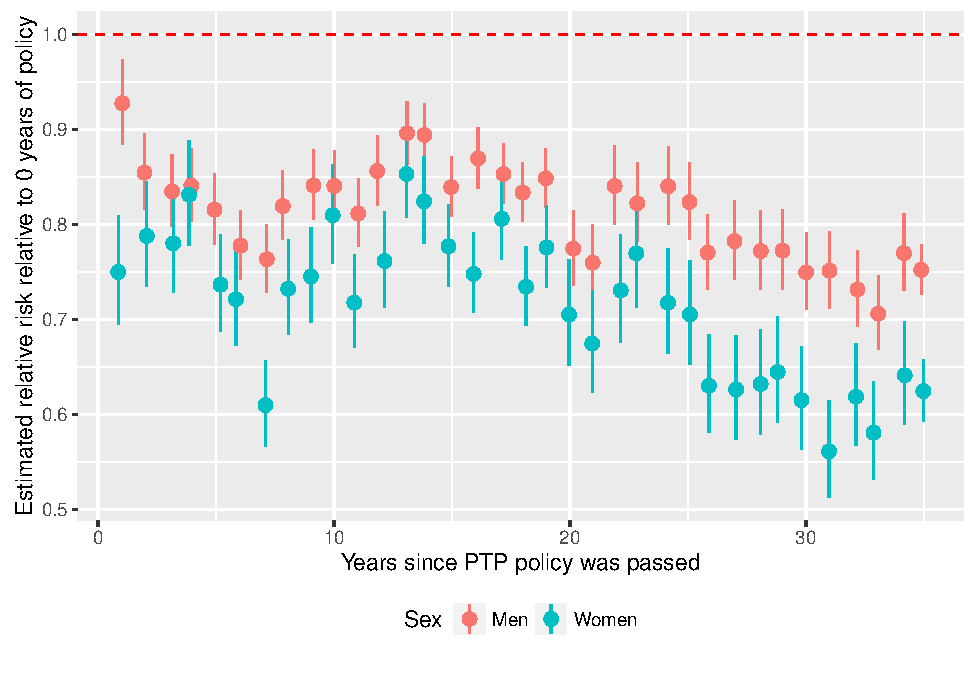
\includegraphics{Thesis_files/figure-latex/supplement-RR-plot-1.pdf}
\caption{Estimated relative risk of non-firearm suicide death by years
since PTP passage for men and women. Point estimates are circles and
95\% confidence intervals are line ranges.}
\end{figure}

When we ran the models with all suicide mortality as the dependent
variable, we found coefficients that were similar to the coefficients
from the main analysis. The results were more similar for men than
women. FUll results of these models are presented in Appendix Table 5.

\subsubsection{Sensitivity Analyses}\label{sensitivity-analyses-1}

We did not observe substantial differences between the full Poisson
model and the alternative negative binomial and zero-inflated Poisson
models. The point estimates of coefficients from the Poisson and
negative binomial models had Pearson correlation coefficients of 0.9997
and 0.9999 for men and women respectively, and the standard errors had a
Pearson correlation coefficients of 1.0000 and 1.0000 for men and women.
Similarly the point estimates of coefficients from the zero-inflated
Poisson model had correlation coefficients of 1.0000 and 0.9999 for men
and women respectively, and the standard errors had a correlation
coefficients of 1.0000 and 1.0000 for men and women. All variables that
were significant in the Poisson model were significant in the other two
models, suggesting that our estimates of the effects of PTP laws were
robust to our choice of likelihood. Scatterplots comparing these models
are in Appendix Figures 6 through 9.

Our results were also not sensitive to our choice of data structure. The
binary parameterization of the exposure variable used in most previous
studies was significant and of a similar magnitude as the indicator
variables in the main analysis. This was unsurprising given that all of
the time-since-passage variables were significant.

Detailed results of the sensitivity analyses are presented in the
Appendix Tables 6 and 7.

\section{Discussion}\label{discussion}

We sought to estimate the effect of state permit-to-purchase
requirements on county-level firearm suicide mortality. We constructed a
dataset that identified the year of every passage or repeal of a state
PTP requirement and used it to generate an indicator variable of
time-since-passage. These indicator variables enabled us to estimate the
effect of PTP requirements more flexibly and robustly than any previous
study in the field. We used a Poisson regression with state and county
random effects to model suicide mortality while controlling for several
frequently used covariates. We found that, among both men and women, PTP
requirements were significantly associated with lower firearm suicide
mortality. The assocaition increased for approximately ten years after
the requirement was introduced before flattening or beginning to
decrease. The resulting curve closely matched our prior expectations
about the dynamics of PTP as a suicide prevention tool despite the
extreme flexibility of the method.

As a secondary analysis, we tested the theory that restricting access to
firearms is an ineffective suicide prevention tool because of
substitution towards other methods. We found no evidence to support this
theory. In fact, increased PTP requirement duration was significantly
associated with decreased non-firearm suicide mortality and decreased
overal suicide mortality.

Previous studies have analyzed the effects of gun control on firearm
mortality rates using a variety of methods and exposure
paramterizations. Excluding the two synthetic control studies described
above, every study reviewed in this paper has constructed its exposure
variables in one of two ways: with composite legislative strength scores
or with a binary variable indicating presence or absence of a particular
policy. Both strategies have their analytical strengths, but neither
lines up particularly well with the theoretical underpinnings of gun
control as a suicide prevention measure.

Without prior information on the relative effectiveness of different
laws, the legislative strength scores are fundamentally arbitrary and
lack the direct policy relevance of specific laws. The scores do create
useful variation between states, but their use limits a study's
interpretability.

Binary exposure variables assign state-years to groups of ``yes'' or
``no''. This approach is appealing if the outcome data have no structure
with respect to time, but without a remarkably diverse set of states in
each group, our ability to filter out cultural ``noise'' is hugely
limited. If we want to make causal claims about the the relationship
between a particular grouping of states and firearm mortality, we need
to be certain that that group of states has nothing else in common that
is not already included in the regression. This is almost certainly
never true. Additionally, regardless of whether or not the binary
variable is ``lagged'' by some number of years, this strategy assumes
that the effect of PTP requirements is constant over policy-time.

By calculating the time since a policy was passed and identifying each
of those durations with an indicator variable, we have generated more
variation between states and removed all assumptions about the
relationship between time since a policy was passed and its effects. For
these reasons, we believe that our method is an improvement on
previously used methodologies. It does require knowledge of when exactly
a given policy was implemented, but that information is far from
unobtainable, as our study has shown.

Our main results exhibited a pattern that was remarkably consistent with
our theoretical expectations and that indicates a strong and signficant
association with our outcome data. We observed an increase in the
effectiveness of PTP requirements at preventing firearm suicides over
approximately the first ten years and a subsequent levelling off.
However, our interpretation of these ostensibly clean results is
complicated by the similarity of the results of the secondary analysis.
We observed a pattern of protective effects against non-firearm suicide
that is undeniably similar to the one we observed in the main analysis.
The theoretical link between restricting firearm access and preventing
non-firearm suicide is tenuous at best. It seems more likely that there
is some source of unaccounted-for confounding we have failed to
consider. It could be that bills that mandate PTP are frequently passed
at similar times as bills that reinforce other suicide prevention
measures, but we did not investigate any other policies, so we cannot
test this theory. Another possible explanation is that there is a
state-specific secular trend that is similar among states with PTP
requirements that we have not accounted for. However, since a particular
policy-time value captures geographically and temporally distant
state-years, correlation across policy-time seems unlikely.

Regardless of why we observed a protective effect in an analysis in
which expected to observe an exacebatory or null effect, we believe that
our results are robust. After controlling for age, year, income,
unemployment, education, and population density and after including
state and county random effects, we still observed highly significant
protective effects of PTP requirements on suicide mortality. Whether or
not this result is \emph{completely} attributable to the PTP
requirement, our exposure is, at the very least, reliably identifying
state-years with systematically lower suicide mortality. Furthermore,
given that the effect of PTP on firearm suicide mortality is greater
than non-firearm suicide, our results are compatible with the theory
that PTP truly is effective.

This study has several important limitations beyond the difficulty of
drawing causal inferences. First, we did not account for the
considerable variation between states in the restrictiveness of their
PTP requirements. As previously discussed, Michigan has much stricter
licensing procedures than Illinois. This variation could be important in
explaining the observed differences.

Additionally, we were unable to control for county- and
municipality-level gun control legislation. If state-level laws affect
suicide mortality, these more local laws must also have an effect. It
was well beyond the scope of this study to assess all firearm
legislation at all levels of government in the US. However, given that
the majority of legislation is still done at the state level and that
several states have passed preemption laws, we do not believe that this
invalidates our main results.

Finally, our analysis is only estimating the impact of PTP requirements
indirectly. As we can see in the conceptual model, the effectiveness of
PTP has two component parts. First, do PTP requirements actually reduce
handgun purchases? And second, does reducing handgun purchases prevent
firearm suicide? Data on handgun ownership are few and far between, so
investigating these questions separately would have been nearly
impossible. Regardless, we believe that by combining these questions and
estimating the net effect of the requirement we have asked a more
policy-relevant question. When members of a state legislature consider
whether or not pass a PTP requirement, the question at hand is not
whether it will directly affect firearm purchases but whether it will
eventually succeed at saving lives. Therefore, it is more sensible to
perform an intent-to-treat type analysis as we have done than to
directly estimate the effect of PTP at each stage of the causal pathway.

Despite the limitations we have identified, we believe that our study
lends support to the theory that PTP requirement could be an effective
suicide prevention tools. The results of our secondary analysis
complicated the interpretation of our main analysis, but we believe that
the relative magnitudes of these results indicate that firearm suicides
are more effectively protected by increased PTP requirement duration
than non-firearm suicides. This effect could be clarified by including
other policy variables in the analysis, but we were unable to find any
such variables.

The body of public health literature examining gun violence in the US is
growing rapidly, but many of these new studies rely on fundamentally
flawed methodologies. Advocates on both sides of the gun control debate
pounce on every newly published study to try to promote their own
interests, so this field demands a particularly high degree of
analytical rigor. Although the primary tool of gun violence prevention
is legislation, we were not able to identify any existing sources that
catalog historical firearm laws. Such an enormous data gap cripples most
researchers' ability to produce high-quality research. We lacked the
resources to compile a comprehensive database of gun control laws over
time, but our analysis demonstrates that it can and should be a priority
for researchers in the field.

\pagebreak  

\section{Appendix}\label{appendix}

\begin{longtable}[c]{@{}rrrrrr@{}}
\caption{History of laws related to PTP requirements in the 50 US states
with statutory sections and bills related to passage and
repeal}\tabularnewline
\toprule
\begin{minipage}[b]{0.10\columnwidth}\raggedleft\strut
State
\strut\end{minipage} &
\begin{minipage}[b]{0.21\columnwidth}\raggedleft\strut
PTP Statute
\strut\end{minipage} &
\begin{minipage}[b]{0.22\columnwidth}\raggedleft\strut
PTP Bill
\strut\end{minipage} &
\begin{minipage}[b]{0.10\columnwidth}\raggedleft\strut
Year Passed
\strut\end{minipage} &
\begin{minipage}[b]{0.10\columnwidth}\raggedleft\strut
Repeal Bill
\strut\end{minipage} &
\begin{minipage}[b]{0.10\columnwidth}\raggedleft\strut
Year Repealed
\strut\end{minipage}\tabularnewline
\midrule
\endfirsthead
\toprule
\begin{minipage}[b]{0.10\columnwidth}\raggedleft\strut
State
\strut\end{minipage} &
\begin{minipage}[b]{0.21\columnwidth}\raggedleft\strut
PTP Statute
\strut\end{minipage} &
\begin{minipage}[b]{0.22\columnwidth}\raggedleft\strut
PTP Bill
\strut\end{minipage} &
\begin{minipage}[b]{0.10\columnwidth}\raggedleft\strut
Year Passed
\strut\end{minipage} &
\begin{minipage}[b]{0.10\columnwidth}\raggedleft\strut
Repeal Bill
\strut\end{minipage} &
\begin{minipage}[b]{0.10\columnwidth}\raggedleft\strut
Year Repealed
\strut\end{minipage}\tabularnewline
\midrule
\endhead
\begin{minipage}[t]{0.10\columnwidth}\raggedleft\strut
Alabama
\strut\end{minipage} &
\begin{minipage}[t]{0.21\columnwidth}\raggedleft\strut
-
\strut\end{minipage} &
\begin{minipage}[t]{0.22\columnwidth}\raggedleft\strut
-
\strut\end{minipage} &
\begin{minipage}[t]{0.10\columnwidth}\raggedleft\strut
-
\strut\end{minipage} &
\begin{minipage}[t]{0.10\columnwidth}\raggedleft\strut
-
\strut\end{minipage} &
\begin{minipage}[t]{0.10\columnwidth}\raggedleft\strut
-
\strut\end{minipage}\tabularnewline
\begin{minipage}[t]{0.10\columnwidth}\raggedleft\strut
Alaska
\strut\end{minipage} &
\begin{minipage}[t]{0.21\columnwidth}\raggedleft\strut
-
\strut\end{minipage} &
\begin{minipage}[t]{0.22\columnwidth}\raggedleft\strut
-
\strut\end{minipage} &
\begin{minipage}[t]{0.10\columnwidth}\raggedleft\strut
-
\strut\end{minipage} &
\begin{minipage}[t]{0.10\columnwidth}\raggedleft\strut
-
\strut\end{minipage} &
\begin{minipage}[t]{0.10\columnwidth}\raggedleft\strut
-
\strut\end{minipage}\tabularnewline
\begin{minipage}[t]{0.10\columnwidth}\raggedleft\strut
Arizona
\strut\end{minipage} &
\begin{minipage}[t]{0.21\columnwidth}\raggedleft\strut
-
\strut\end{minipage} &
\begin{minipage}[t]{0.22\columnwidth}\raggedleft\strut
-
\strut\end{minipage} &
\begin{minipage}[t]{0.10\columnwidth}\raggedleft\strut
-
\strut\end{minipage} &
\begin{minipage}[t]{0.10\columnwidth}\raggedleft\strut
-
\strut\end{minipage} &
\begin{minipage}[t]{0.10\columnwidth}\raggedleft\strut
-
\strut\end{minipage}\tabularnewline
\begin{minipage}[t]{0.10\columnwidth}\raggedleft\strut
Arkansas
\strut\end{minipage} &
\begin{minipage}[t]{0.21\columnwidth}\raggedleft\strut
-
\strut\end{minipage} &
\begin{minipage}[t]{0.22\columnwidth}\raggedleft\strut
-
\strut\end{minipage} &
\begin{minipage}[t]{0.10\columnwidth}\raggedleft\strut
-
\strut\end{minipage} &
\begin{minipage}[t]{0.10\columnwidth}\raggedleft\strut
-
\strut\end{minipage} &
\begin{minipage}[t]{0.10\columnwidth}\raggedleft\strut
-
\strut\end{minipage}\tabularnewline
\begin{minipage}[t]{0.10\columnwidth}\raggedleft\strut
California
\strut\end{minipage} &
\begin{minipage}[t]{0.21\columnwidth}\raggedleft\strut
Cal Pen Code § 26500, Cal Pen Code § 12070
\strut\end{minipage} &
\begin{minipage}[t]{0.22\columnwidth}\raggedleft\strut
Stats 2010 ch 711 § 6 (SB 1080),
\strut\end{minipage} &
\begin{minipage}[t]{0.10\columnwidth}\raggedleft\strut
1994
\strut\end{minipage} &
\begin{minipage}[t]{0.10\columnwidth}\raggedleft\strut
-
\strut\end{minipage} &
\begin{minipage}[t]{0.10\columnwidth}\raggedleft\strut
-
\strut\end{minipage}\tabularnewline
\begin{minipage}[t]{0.10\columnwidth}\raggedleft\strut
Colorado
\strut\end{minipage} &
\begin{minipage}[t]{0.21\columnwidth}\raggedleft\strut
-
\strut\end{minipage} &
\begin{minipage}[t]{0.22\columnwidth}\raggedleft\strut
-
\strut\end{minipage} &
\begin{minipage}[t]{0.10\columnwidth}\raggedleft\strut
-
\strut\end{minipage} &
\begin{minipage}[t]{0.10\columnwidth}\raggedleft\strut
-
\strut\end{minipage} &
\begin{minipage}[t]{0.10\columnwidth}\raggedleft\strut
-
\strut\end{minipage}\tabularnewline
\begin{minipage}[t]{0.10\columnwidth}\raggedleft\strut
Connecticut
\strut\end{minipage} &
\begin{minipage}[t]{0.21\columnwidth}\raggedleft\strut
Conn. Gen.~Stat. § 29-36f
\strut\end{minipage} &
\begin{minipage}[t]{0.22\columnwidth}\raggedleft\strut
July Sp. Sess. P.A. 94-1, S. 7.
\strut\end{minipage} &
\begin{minipage}[t]{0.10\columnwidth}\raggedleft\strut
1994
\strut\end{minipage} &
\begin{minipage}[t]{0.10\columnwidth}\raggedleft\strut
-
\strut\end{minipage} &
\begin{minipage}[t]{0.10\columnwidth}\raggedleft\strut
-
\strut\end{minipage}\tabularnewline
\begin{minipage}[t]{0.10\columnwidth}\raggedleft\strut
Delaware
\strut\end{minipage} &
\begin{minipage}[t]{0.21\columnwidth}\raggedleft\strut
-
\strut\end{minipage} &
\begin{minipage}[t]{0.22\columnwidth}\raggedleft\strut
-
\strut\end{minipage} &
\begin{minipage}[t]{0.10\columnwidth}\raggedleft\strut
-
\strut\end{minipage} &
\begin{minipage}[t]{0.10\columnwidth}\raggedleft\strut
-
\strut\end{minipage} &
\begin{minipage}[t]{0.10\columnwidth}\raggedleft\strut
-
\strut\end{minipage}\tabularnewline
\begin{minipage}[t]{0.10\columnwidth}\raggedleft\strut
Florida
\strut\end{minipage} &
\begin{minipage}[t]{0.21\columnwidth}\raggedleft\strut
-
\strut\end{minipage} &
\begin{minipage}[t]{0.22\columnwidth}\raggedleft\strut
-
\strut\end{minipage} &
\begin{minipage}[t]{0.10\columnwidth}\raggedleft\strut
-
\strut\end{minipage} &
\begin{minipage}[t]{0.10\columnwidth}\raggedleft\strut
-
\strut\end{minipage} &
\begin{minipage}[t]{0.10\columnwidth}\raggedleft\strut
-
\strut\end{minipage}\tabularnewline
\begin{minipage}[t]{0.10\columnwidth}\raggedleft\strut
Georgia
\strut\end{minipage} &
\begin{minipage}[t]{0.21\columnwidth}\raggedleft\strut
-
\strut\end{minipage} &
\begin{minipage}[t]{0.22\columnwidth}\raggedleft\strut
-
\strut\end{minipage} &
\begin{minipage}[t]{0.10\columnwidth}\raggedleft\strut
-
\strut\end{minipage} &
\begin{minipage}[t]{0.10\columnwidth}\raggedleft\strut
-
\strut\end{minipage} &
\begin{minipage}[t]{0.10\columnwidth}\raggedleft\strut
-
\strut\end{minipage}\tabularnewline
\begin{minipage}[t]{0.10\columnwidth}\raggedleft\strut
Hawaii
\strut\end{minipage} &
\begin{minipage}[t]{0.21\columnwidth}\raggedleft\strut
HRS §~134-2
\strut\end{minipage} &
\begin{minipage}[t]{0.22\columnwidth}\raggedleft\strut
L 1988, c 275, pt of § 2
\strut\end{minipage} &
\begin{minipage}[t]{0.10\columnwidth}\raggedleft\strut
1988
\strut\end{minipage} &
\begin{minipage}[t]{0.10\columnwidth}\raggedleft\strut
-
\strut\end{minipage} &
\begin{minipage}[t]{0.10\columnwidth}\raggedleft\strut
-
\strut\end{minipage}\tabularnewline
\begin{minipage}[t]{0.10\columnwidth}\raggedleft\strut
Idaho
\strut\end{minipage} &
\begin{minipage}[t]{0.21\columnwidth}\raggedleft\strut
-
\strut\end{minipage} &
\begin{minipage}[t]{0.22\columnwidth}\raggedleft\strut
-
\strut\end{minipage} &
\begin{minipage}[t]{0.10\columnwidth}\raggedleft\strut
-
\strut\end{minipage} &
\begin{minipage}[t]{0.10\columnwidth}\raggedleft\strut
-
\strut\end{minipage} &
\begin{minipage}[t]{0.10\columnwidth}\raggedleft\strut
-
\strut\end{minipage}\tabularnewline
\begin{minipage}[t]{0.10\columnwidth}\raggedleft\strut
Illinois
\strut\end{minipage} &
\begin{minipage}[t]{0.21\columnwidth}\raggedleft\strut
430 ILCS 65/2
\strut\end{minipage} &
\begin{minipage}[t]{0.22\columnwidth}\raggedleft\strut
Laws 1967, p.~2600
\strut\end{minipage} &
\begin{minipage}[t]{0.10\columnwidth}\raggedleft\strut
1967
\strut\end{minipage} &
\begin{minipage}[t]{0.10\columnwidth}\raggedleft\strut
-
\strut\end{minipage} &
\begin{minipage}[t]{0.10\columnwidth}\raggedleft\strut
-
\strut\end{minipage}\tabularnewline
\begin{minipage}[t]{0.10\columnwidth}\raggedleft\strut
Indiana
\strut\end{minipage} &
\begin{minipage}[t]{0.21\columnwidth}\raggedleft\strut
-
\strut\end{minipage} &
\begin{minipage}[t]{0.22\columnwidth}\raggedleft\strut
-
\strut\end{minipage} &
\begin{minipage}[t]{0.10\columnwidth}\raggedleft\strut
-
\strut\end{minipage} &
\begin{minipage}[t]{0.10\columnwidth}\raggedleft\strut
-
\strut\end{minipage} &
\begin{minipage}[t]{0.10\columnwidth}\raggedleft\strut
-
\strut\end{minipage}\tabularnewline
\begin{minipage}[t]{0.10\columnwidth}\raggedleft\strut
Iowa
\strut\end{minipage} &
\begin{minipage}[t]{0.21\columnwidth}\raggedleft\strut
Iowa Code § 724.15
\strut\end{minipage} &
\begin{minipage}[t]{0.22\columnwidth}\raggedleft\strut
C79, 81, § 724.15
\strut\end{minipage} &
\begin{minipage}[t]{0.10\columnwidth}\raggedleft\strut
1979
\strut\end{minipage} &
\begin{minipage}[t]{0.10\columnwidth}\raggedleft\strut
-
\strut\end{minipage} &
\begin{minipage}[t]{0.10\columnwidth}\raggedleft\strut
-
\strut\end{minipage}\tabularnewline
\begin{minipage}[t]{0.10\columnwidth}\raggedleft\strut
Kansas
\strut\end{minipage} &
\begin{minipage}[t]{0.21\columnwidth}\raggedleft\strut
-
\strut\end{minipage} &
\begin{minipage}[t]{0.22\columnwidth}\raggedleft\strut
-
\strut\end{minipage} &
\begin{minipage}[t]{0.10\columnwidth}\raggedleft\strut
-
\strut\end{minipage} &
\begin{minipage}[t]{0.10\columnwidth}\raggedleft\strut
-
\strut\end{minipage} &
\begin{minipage}[t]{0.10\columnwidth}\raggedleft\strut
-
\strut\end{minipage}\tabularnewline
\begin{minipage}[t]{0.10\columnwidth}\raggedleft\strut
Kentucky
\strut\end{minipage} &
\begin{minipage}[t]{0.21\columnwidth}\raggedleft\strut
-
\strut\end{minipage} &
\begin{minipage}[t]{0.22\columnwidth}\raggedleft\strut
-
\strut\end{minipage} &
\begin{minipage}[t]{0.10\columnwidth}\raggedleft\strut
-
\strut\end{minipage} &
\begin{minipage}[t]{0.10\columnwidth}\raggedleft\strut
-
\strut\end{minipage} &
\begin{minipage}[t]{0.10\columnwidth}\raggedleft\strut
-
\strut\end{minipage}\tabularnewline
\begin{minipage}[t]{0.10\columnwidth}\raggedleft\strut
Louisiana
\strut\end{minipage} &
\begin{minipage}[t]{0.21\columnwidth}\raggedleft\strut
-
\strut\end{minipage} &
\begin{minipage}[t]{0.22\columnwidth}\raggedleft\strut
-
\strut\end{minipage} &
\begin{minipage}[t]{0.10\columnwidth}\raggedleft\strut
-
\strut\end{minipage} &
\begin{minipage}[t]{0.10\columnwidth}\raggedleft\strut
-
\strut\end{minipage} &
\begin{minipage}[t]{0.10\columnwidth}\raggedleft\strut
-
\strut\end{minipage}\tabularnewline
\begin{minipage}[t]{0.10\columnwidth}\raggedleft\strut
Maine
\strut\end{minipage} &
\begin{minipage}[t]{0.21\columnwidth}\raggedleft\strut
-
\strut\end{minipage} &
\begin{minipage}[t]{0.22\columnwidth}\raggedleft\strut
-
\strut\end{minipage} &
\begin{minipage}[t]{0.10\columnwidth}\raggedleft\strut
-
\strut\end{minipage} &
\begin{minipage}[t]{0.10\columnwidth}\raggedleft\strut
-
\strut\end{minipage} &
\begin{minipage}[t]{0.10\columnwidth}\raggedleft\strut
-
\strut\end{minipage}\tabularnewline
\begin{minipage}[t]{0.10\columnwidth}\raggedleft\strut
Maryland
\strut\end{minipage} &
\begin{minipage}[t]{0.21\columnwidth}\raggedleft\strut
Md. PUBLIC SAFETY Code Ann. § 5-117.1
\strut\end{minipage} &
\begin{minipage}[t]{0.22\columnwidth}\raggedleft\strut
2013 Md. ALS 427
\strut\end{minipage} &
\begin{minipage}[t]{0.10\columnwidth}\raggedleft\strut
2013
\strut\end{minipage} &
\begin{minipage}[t]{0.10\columnwidth}\raggedleft\strut
-
\strut\end{minipage} &
\begin{minipage}[t]{0.10\columnwidth}\raggedleft\strut
-
\strut\end{minipage}\tabularnewline
\begin{minipage}[t]{0.10\columnwidth}\raggedleft\strut
Massachusetts
\strut\end{minipage} &
\begin{minipage}[t]{0.21\columnwidth}\raggedleft\strut
ALM GL ch.~140, § 131
\strut\end{minipage} &
\begin{minipage}[t]{0.22\columnwidth}\raggedleft\strut
-
\strut\end{minipage} &
\begin{minipage}[t]{0.10\columnwidth}\raggedleft\strut
1906
\strut\end{minipage} &
\begin{minipage}[t]{0.10\columnwidth}\raggedleft\strut
-
\strut\end{minipage} &
\begin{minipage}[t]{0.10\columnwidth}\raggedleft\strut
-
\strut\end{minipage}\tabularnewline
\begin{minipage}[t]{0.10\columnwidth}\raggedleft\strut
Michigan
\strut\end{minipage} &
\begin{minipage}[t]{0.21\columnwidth}\raggedleft\strut
MCLS § 28.422
\strut\end{minipage} &
\begin{minipage}[t]{0.22\columnwidth}\raggedleft\strut
Pub Acts 1927, No. 372, § 2
\strut\end{minipage} &
\begin{minipage}[t]{0.10\columnwidth}\raggedleft\strut
1927
\strut\end{minipage} &
\begin{minipage}[t]{0.10\columnwidth}\raggedleft\strut
-
\strut\end{minipage} &
\begin{minipage}[t]{0.10\columnwidth}\raggedleft\strut
-
\strut\end{minipage}\tabularnewline
\begin{minipage}[t]{0.10\columnwidth}\raggedleft\strut
Minnesota
\strut\end{minipage} &
\begin{minipage}[t]{0.21\columnwidth}\raggedleft\strut
Minn. Stat. § 624.7131
\strut\end{minipage} &
\begin{minipage}[t]{0.22\columnwidth}\raggedleft\strut
1977 c 349 s 4
\strut\end{minipage} &
\begin{minipage}[t]{0.10\columnwidth}\raggedleft\strut
1977
\strut\end{minipage} &
\begin{minipage}[t]{0.10\columnwidth}\raggedleft\strut
-
\strut\end{minipage} &
\begin{minipage}[t]{0.10\columnwidth}\raggedleft\strut
-
\strut\end{minipage}\tabularnewline
\begin{minipage}[t]{0.10\columnwidth}\raggedleft\strut
Mississippi
\strut\end{minipage} &
\begin{minipage}[t]{0.21\columnwidth}\raggedleft\strut
-
\strut\end{minipage} &
\begin{minipage}[t]{0.22\columnwidth}\raggedleft\strut
-
\strut\end{minipage} &
\begin{minipage}[t]{0.10\columnwidth}\raggedleft\strut
-
\strut\end{minipage} &
\begin{minipage}[t]{0.10\columnwidth}\raggedleft\strut
-
\strut\end{minipage} &
\begin{minipage}[t]{0.10\columnwidth}\raggedleft\strut
-
\strut\end{minipage}\tabularnewline
\begin{minipage}[t]{0.10\columnwidth}\raggedleft\strut
Missouri
\strut\end{minipage} &
\begin{minipage}[t]{0.21\columnwidth}\raggedleft\strut
§ 571.080 R.S.Mo.
\strut\end{minipage} &
\begin{minipage}[t]{0.22\columnwidth}\raggedleft\strut
L. 1981 H.B. 296 subsecs. 1, 2, 3
\strut\end{minipage} &
\begin{minipage}[t]{0.10\columnwidth}\raggedleft\strut
1981
\strut\end{minipage} &
\begin{minipage}[t]{0.10\columnwidth}\raggedleft\strut
2007 Mo. SB 62
\strut\end{minipage} &
\begin{minipage}[t]{0.10\columnwidth}\raggedleft\strut
2007
\strut\end{minipage}\tabularnewline
\begin{minipage}[t]{0.10\columnwidth}\raggedleft\strut
Montana
\strut\end{minipage} &
\begin{minipage}[t]{0.21\columnwidth}\raggedleft\strut
-
\strut\end{minipage} &
\begin{minipage}[t]{0.22\columnwidth}\raggedleft\strut
-
\strut\end{minipage} &
\begin{minipage}[t]{0.10\columnwidth}\raggedleft\strut
-
\strut\end{minipage} &
\begin{minipage}[t]{0.10\columnwidth}\raggedleft\strut
-
\strut\end{minipage} &
\begin{minipage}[t]{0.10\columnwidth}\raggedleft\strut
-
\strut\end{minipage}\tabularnewline
\begin{minipage}[t]{0.10\columnwidth}\raggedleft\strut
Nebraska
\strut\end{minipage} &
\begin{minipage}[t]{0.21\columnwidth}\raggedleft\strut
R.R.S. Neb. § 69-2403
\strut\end{minipage} &
\begin{minipage}[t]{0.22\columnwidth}\raggedleft\strut
Laws 1991, LB 355, § 2
\strut\end{minipage} &
\begin{minipage}[t]{0.10\columnwidth}\raggedleft\strut
1991
\strut\end{minipage} &
\begin{minipage}[t]{0.10\columnwidth}\raggedleft\strut
-
\strut\end{minipage} &
\begin{minipage}[t]{0.10\columnwidth}\raggedleft\strut
-
\strut\end{minipage}\tabularnewline
\begin{minipage}[t]{0.10\columnwidth}\raggedleft\strut
Nevada
\strut\end{minipage} &
\begin{minipage}[t]{0.21\columnwidth}\raggedleft\strut
-
\strut\end{minipage} &
\begin{minipage}[t]{0.22\columnwidth}\raggedleft\strut
-
\strut\end{minipage} &
\begin{minipage}[t]{0.10\columnwidth}\raggedleft\strut
-
\strut\end{minipage} &
\begin{minipage}[t]{0.10\columnwidth}\raggedleft\strut
-
\strut\end{minipage} &
\begin{minipage}[t]{0.10\columnwidth}\raggedleft\strut
-
\strut\end{minipage}\tabularnewline
\begin{minipage}[t]{0.10\columnwidth}\raggedleft\strut
New Hampshire
\strut\end{minipage} &
\begin{minipage}[t]{0.21\columnwidth}\raggedleft\strut
-
\strut\end{minipage} &
\begin{minipage}[t]{0.22\columnwidth}\raggedleft\strut
-
\strut\end{minipage} &
\begin{minipage}[t]{0.10\columnwidth}\raggedleft\strut
-
\strut\end{minipage} &
\begin{minipage}[t]{0.10\columnwidth}\raggedleft\strut
-
\strut\end{minipage} &
\begin{minipage}[t]{0.10\columnwidth}\raggedleft\strut
-
\strut\end{minipage}\tabularnewline
\begin{minipage}[t]{0.10\columnwidth}\raggedleft\strut
New Jersey
\strut\end{minipage} &
\begin{minipage}[t]{0.21\columnwidth}\raggedleft\strut
N.J. Stat. § 2C:58-3
\strut\end{minipage} &
\begin{minipage}[t]{0.22\columnwidth}\raggedleft\strut
L. 1978, c. 95
\strut\end{minipage} &
\begin{minipage}[t]{0.10\columnwidth}\raggedleft\strut
1978
\strut\end{minipage} &
\begin{minipage}[t]{0.10\columnwidth}\raggedleft\strut
-
\strut\end{minipage} &
\begin{minipage}[t]{0.10\columnwidth}\raggedleft\strut
-
\strut\end{minipage}\tabularnewline
\begin{minipage}[t]{0.10\columnwidth}\raggedleft\strut
New Mexico
\strut\end{minipage} &
\begin{minipage}[t]{0.21\columnwidth}\raggedleft\strut
-
\strut\end{minipage} &
\begin{minipage}[t]{0.22\columnwidth}\raggedleft\strut
-
\strut\end{minipage} &
\begin{minipage}[t]{0.10\columnwidth}\raggedleft\strut
-
\strut\end{minipage} &
\begin{minipage}[t]{0.10\columnwidth}\raggedleft\strut
-
\strut\end{minipage} &
\begin{minipage}[t]{0.10\columnwidth}\raggedleft\strut
-
\strut\end{minipage}\tabularnewline
\begin{minipage}[t]{0.10\columnwidth}\raggedleft\strut
New York
\strut\end{minipage} &
\begin{minipage}[t]{0.21\columnwidth}\raggedleft\strut
NY CLS Penal § 400.00
\strut\end{minipage} &
\begin{minipage}[t]{0.22\columnwidth}\raggedleft\strut
L 1965, ch 1030, § 1, eff Sept 1, 1967
\strut\end{minipage} &
\begin{minipage}[t]{0.10\columnwidth}\raggedleft\strut
1967
\strut\end{minipage} &
\begin{minipage}[t]{0.10\columnwidth}\raggedleft\strut
-
\strut\end{minipage} &
\begin{minipage}[t]{0.10\columnwidth}\raggedleft\strut
-
\strut\end{minipage}\tabularnewline
\begin{minipage}[t]{0.10\columnwidth}\raggedleft\strut
North Carolina
\strut\end{minipage} &
\begin{minipage}[t]{0.21\columnwidth}\raggedleft\strut
N.C. Gen.~Stat. § 14-402
\strut\end{minipage} &
\begin{minipage}[t]{0.22\columnwidth}\raggedleft\strut
1919, c. 197
\strut\end{minipage} &
\begin{minipage}[t]{0.10\columnwidth}\raggedleft\strut
1919
\strut\end{minipage} &
\begin{minipage}[t]{0.10\columnwidth}\raggedleft\strut
-
\strut\end{minipage} &
\begin{minipage}[t]{0.10\columnwidth}\raggedleft\strut
-
\strut\end{minipage}\tabularnewline
\begin{minipage}[t]{0.10\columnwidth}\raggedleft\strut
North Dakota
\strut\end{minipage} &
\begin{minipage}[t]{0.21\columnwidth}\raggedleft\strut
-
\strut\end{minipage} &
\begin{minipage}[t]{0.22\columnwidth}\raggedleft\strut
-
\strut\end{minipage} &
\begin{minipage}[t]{0.10\columnwidth}\raggedleft\strut
-
\strut\end{minipage} &
\begin{minipage}[t]{0.10\columnwidth}\raggedleft\strut
-
\strut\end{minipage} &
\begin{minipage}[t]{0.10\columnwidth}\raggedleft\strut
-
\strut\end{minipage}\tabularnewline
\begin{minipage}[t]{0.10\columnwidth}\raggedleft\strut
Ohio
\strut\end{minipage} &
\begin{minipage}[t]{0.21\columnwidth}\raggedleft\strut
-
\strut\end{minipage} &
\begin{minipage}[t]{0.22\columnwidth}\raggedleft\strut
-
\strut\end{minipage} &
\begin{minipage}[t]{0.10\columnwidth}\raggedleft\strut
-
\strut\end{minipage} &
\begin{minipage}[t]{0.10\columnwidth}\raggedleft\strut
-
\strut\end{minipage} &
\begin{minipage}[t]{0.10\columnwidth}\raggedleft\strut
-
\strut\end{minipage}\tabularnewline
\begin{minipage}[t]{0.10\columnwidth}\raggedleft\strut
Oklahoma
\strut\end{minipage} &
\begin{minipage}[t]{0.21\columnwidth}\raggedleft\strut
-
\strut\end{minipage} &
\begin{minipage}[t]{0.22\columnwidth}\raggedleft\strut
-
\strut\end{minipage} &
\begin{minipage}[t]{0.10\columnwidth}\raggedleft\strut
-
\strut\end{minipage} &
\begin{minipage}[t]{0.10\columnwidth}\raggedleft\strut
-
\strut\end{minipage} &
\begin{minipage}[t]{0.10\columnwidth}\raggedleft\strut
-
\strut\end{minipage}\tabularnewline
\begin{minipage}[t]{0.10\columnwidth}\raggedleft\strut
Oregon
\strut\end{minipage} &
\begin{minipage}[t]{0.21\columnwidth}\raggedleft\strut
-
\strut\end{minipage} &
\begin{minipage}[t]{0.22\columnwidth}\raggedleft\strut
-
\strut\end{minipage} &
\begin{minipage}[t]{0.10\columnwidth}\raggedleft\strut
-
\strut\end{minipage} &
\begin{minipage}[t]{0.10\columnwidth}\raggedleft\strut
-
\strut\end{minipage} &
\begin{minipage}[t]{0.10\columnwidth}\raggedleft\strut
-
\strut\end{minipage}\tabularnewline
\begin{minipage}[t]{0.10\columnwidth}\raggedleft\strut
Pennsylvania
\strut\end{minipage} &
\begin{minipage}[t]{0.21\columnwidth}\raggedleft\strut
-
\strut\end{minipage} &
\begin{minipage}[t]{0.22\columnwidth}\raggedleft\strut
-
\strut\end{minipage} &
\begin{minipage}[t]{0.10\columnwidth}\raggedleft\strut
-
\strut\end{minipage} &
\begin{minipage}[t]{0.10\columnwidth}\raggedleft\strut
-
\strut\end{minipage} &
\begin{minipage}[t]{0.10\columnwidth}\raggedleft\strut
-
\strut\end{minipage}\tabularnewline
\begin{minipage}[t]{0.10\columnwidth}\raggedleft\strut
Rhode Island
\strut\end{minipage} &
\begin{minipage}[t]{0.21\columnwidth}\raggedleft\strut
R.I. Gen.~Laws § 11-47-35
\strut\end{minipage} &
\begin{minipage}[t]{0.22\columnwidth}\raggedleft\strut
G.L. 1956 (1981 Reenactment) § 11-47-35
\strut\end{minipage} &
\begin{minipage}[t]{0.10\columnwidth}\raggedleft\strut
1956
\strut\end{minipage} &
\begin{minipage}[t]{0.10\columnwidth}\raggedleft\strut
-
\strut\end{minipage} &
\begin{minipage}[t]{0.10\columnwidth}\raggedleft\strut
-
\strut\end{minipage}\tabularnewline
\begin{minipage}[t]{0.10\columnwidth}\raggedleft\strut
South Carolina
\strut\end{minipage} &
\begin{minipage}[t]{0.21\columnwidth}\raggedleft\strut
-
\strut\end{minipage} &
\begin{minipage}[t]{0.22\columnwidth}\raggedleft\strut
-
\strut\end{minipage} &
\begin{minipage}[t]{0.10\columnwidth}\raggedleft\strut
-
\strut\end{minipage} &
\begin{minipage}[t]{0.10\columnwidth}\raggedleft\strut
-
\strut\end{minipage} &
\begin{minipage}[t]{0.10\columnwidth}\raggedleft\strut
-
\strut\end{minipage}\tabularnewline
\begin{minipage}[t]{0.10\columnwidth}\raggedleft\strut
South Dakota
\strut\end{minipage} &
\begin{minipage}[t]{0.21\columnwidth}\raggedleft\strut
-
\strut\end{minipage} &
\begin{minipage}[t]{0.22\columnwidth}\raggedleft\strut
-
\strut\end{minipage} &
\begin{minipage}[t]{0.10\columnwidth}\raggedleft\strut
-
\strut\end{minipage} &
\begin{minipage}[t]{0.10\columnwidth}\raggedleft\strut
-
\strut\end{minipage} &
\begin{minipage}[t]{0.10\columnwidth}\raggedleft\strut
-
\strut\end{minipage}\tabularnewline
\begin{minipage}[t]{0.10\columnwidth}\raggedleft\strut
Tennessee
\strut\end{minipage} &
\begin{minipage}[t]{0.21\columnwidth}\raggedleft\strut
-
\strut\end{minipage} &
\begin{minipage}[t]{0.22\columnwidth}\raggedleft\strut
-
\strut\end{minipage} &
\begin{minipage}[t]{0.10\columnwidth}\raggedleft\strut
-
\strut\end{minipage} &
\begin{minipage}[t]{0.10\columnwidth}\raggedleft\strut
-
\strut\end{minipage} &
\begin{minipage}[t]{0.10\columnwidth}\raggedleft\strut
-
\strut\end{minipage}\tabularnewline
\begin{minipage}[t]{0.10\columnwidth}\raggedleft\strut
Texas
\strut\end{minipage} &
\begin{minipage}[t]{0.21\columnwidth}\raggedleft\strut
-
\strut\end{minipage} &
\begin{minipage}[t]{0.22\columnwidth}\raggedleft\strut
-
\strut\end{minipage} &
\begin{minipage}[t]{0.10\columnwidth}\raggedleft\strut
-
\strut\end{minipage} &
\begin{minipage}[t]{0.10\columnwidth}\raggedleft\strut
-
\strut\end{minipage} &
\begin{minipage}[t]{0.10\columnwidth}\raggedleft\strut
-
\strut\end{minipage}\tabularnewline
\begin{minipage}[t]{0.10\columnwidth}\raggedleft\strut
Utah
\strut\end{minipage} &
\begin{minipage}[t]{0.21\columnwidth}\raggedleft\strut
-
\strut\end{minipage} &
\begin{minipage}[t]{0.22\columnwidth}\raggedleft\strut
-
\strut\end{minipage} &
\begin{minipage}[t]{0.10\columnwidth}\raggedleft\strut
-
\strut\end{minipage} &
\begin{minipage}[t]{0.10\columnwidth}\raggedleft\strut
-
\strut\end{minipage} &
\begin{minipage}[t]{0.10\columnwidth}\raggedleft\strut
-
\strut\end{minipage}\tabularnewline
\begin{minipage}[t]{0.10\columnwidth}\raggedleft\strut
Vermont
\strut\end{minipage} &
\begin{minipage}[t]{0.21\columnwidth}\raggedleft\strut
-
\strut\end{minipage} &
\begin{minipage}[t]{0.22\columnwidth}\raggedleft\strut
-
\strut\end{minipage} &
\begin{minipage}[t]{0.10\columnwidth}\raggedleft\strut
-
\strut\end{minipage} &
\begin{minipage}[t]{0.10\columnwidth}\raggedleft\strut
-
\strut\end{minipage} &
\begin{minipage}[t]{0.10\columnwidth}\raggedleft\strut
-
\strut\end{minipage}\tabularnewline
\begin{minipage}[t]{0.10\columnwidth}\raggedleft\strut
Virginia
\strut\end{minipage} &
\begin{minipage}[t]{0.21\columnwidth}\raggedleft\strut
-
\strut\end{minipage} &
\begin{minipage}[t]{0.22\columnwidth}\raggedleft\strut
-
\strut\end{minipage} &
\begin{minipage}[t]{0.10\columnwidth}\raggedleft\strut
-
\strut\end{minipage} &
\begin{minipage}[t]{0.10\columnwidth}\raggedleft\strut
-
\strut\end{minipage} &
\begin{minipage}[t]{0.10\columnwidth}\raggedleft\strut
-
\strut\end{minipage}\tabularnewline
\begin{minipage}[t]{0.10\columnwidth}\raggedleft\strut
Washington
\strut\end{minipage} &
\begin{minipage}[t]{0.21\columnwidth}\raggedleft\strut
-
\strut\end{minipage} &
\begin{minipage}[t]{0.22\columnwidth}\raggedleft\strut
-
\strut\end{minipage} &
\begin{minipage}[t]{0.10\columnwidth}\raggedleft\strut
-
\strut\end{minipage} &
\begin{minipage}[t]{0.10\columnwidth}\raggedleft\strut
-
\strut\end{minipage} &
\begin{minipage}[t]{0.10\columnwidth}\raggedleft\strut
-
\strut\end{minipage}\tabularnewline
\begin{minipage}[t]{0.10\columnwidth}\raggedleft\strut
West Virginia
\strut\end{minipage} &
\begin{minipage}[t]{0.21\columnwidth}\raggedleft\strut
-
\strut\end{minipage} &
\begin{minipage}[t]{0.22\columnwidth}\raggedleft\strut
-
\strut\end{minipage} &
\begin{minipage}[t]{0.10\columnwidth}\raggedleft\strut
-
\strut\end{minipage} &
\begin{minipage}[t]{0.10\columnwidth}\raggedleft\strut
-
\strut\end{minipage} &
\begin{minipage}[t]{0.10\columnwidth}\raggedleft\strut
-
\strut\end{minipage}\tabularnewline
\begin{minipage}[t]{0.10\columnwidth}\raggedleft\strut
Wisconsin
\strut\end{minipage} &
\begin{minipage}[t]{0.21\columnwidth}\raggedleft\strut
-
\strut\end{minipage} &
\begin{minipage}[t]{0.22\columnwidth}\raggedleft\strut
-
\strut\end{minipage} &
\begin{minipage}[t]{0.10\columnwidth}\raggedleft\strut
-
\strut\end{minipage} &
\begin{minipage}[t]{0.10\columnwidth}\raggedleft\strut
-
\strut\end{minipage} &
\begin{minipage}[t]{0.10\columnwidth}\raggedleft\strut
-
\strut\end{minipage}\tabularnewline
\begin{minipage}[t]{0.10\columnwidth}\raggedleft\strut
Wyoming
\strut\end{minipage} &
\begin{minipage}[t]{0.21\columnwidth}\raggedleft\strut
-
\strut\end{minipage} &
\begin{minipage}[t]{0.22\columnwidth}\raggedleft\strut
-
\strut\end{minipage} &
\begin{minipage}[t]{0.10\columnwidth}\raggedleft\strut
-
\strut\end{minipage} &
\begin{minipage}[t]{0.10\columnwidth}\raggedleft\strut
-
\strut\end{minipage} &
\begin{minipage}[t]{0.10\columnwidth}\raggedleft\strut
-
\strut\end{minipage}\tabularnewline
\bottomrule
\end{longtable}

\pagebreak

\begin{longtable}[c]{@{}rrrrrrr@{}}
\caption{Full results of Poisson regressions with firearm suicide as
dependent variable. Point estimates are coefficients from linear model.
Standard errors are presented in parentheses. One, two, and three
asterisks indicate significance at the 0.05, 0.01, and 0.001 levels
respectively.}\tabularnewline
\toprule
\begin{minipage}[b]{0.12\columnwidth}\raggedleft\strut
Variable
\strut\end{minipage} &
\begin{minipage}[b]{0.11\columnwidth}\raggedleft\strut
Model 1
\strut\end{minipage} &
\begin{minipage}[b]{0.12\columnwidth}\raggedleft\strut
~
\strut\end{minipage} &
\begin{minipage}[b]{0.11\columnwidth}\raggedleft\strut
Model 2
\strut\end{minipage} &
\begin{minipage}[b]{0.12\columnwidth}\raggedleft\strut
~
\strut\end{minipage} &
\begin{minipage}[b]{0.11\columnwidth}\raggedleft\strut
Model 3
\strut\end{minipage} &
\begin{minipage}[b]{0.11\columnwidth}\raggedleft\strut
~
\strut\end{minipage}\tabularnewline
\midrule
\endfirsthead
\toprule
\begin{minipage}[b]{0.12\columnwidth}\raggedleft\strut
Variable
\strut\end{minipage} &
\begin{minipage}[b]{0.11\columnwidth}\raggedleft\strut
Model 1
\strut\end{minipage} &
\begin{minipage}[b]{0.12\columnwidth}\raggedleft\strut
~
\strut\end{minipage} &
\begin{minipage}[b]{0.11\columnwidth}\raggedleft\strut
Model 2
\strut\end{minipage} &
\begin{minipage}[b]{0.12\columnwidth}\raggedleft\strut
~
\strut\end{minipage} &
\begin{minipage}[b]{0.11\columnwidth}\raggedleft\strut
Model 3
\strut\end{minipage} &
\begin{minipage}[b]{0.11\columnwidth}\raggedleft\strut
~
\strut\end{minipage}\tabularnewline
\midrule
\endhead
\begin{minipage}[t]{0.12\columnwidth}\raggedleft\strut
\strut\end{minipage} &
\begin{minipage}[t]{0.11\columnwidth}\raggedleft\strut
\textbf{Men}
\strut\end{minipage} &
\begin{minipage}[t]{0.12\columnwidth}\raggedleft\strut
\textbf{Women}
\strut\end{minipage} &
\begin{minipage}[t]{0.11\columnwidth}\raggedleft\strut
\textbf{Men}
\strut\end{minipage} &
\begin{minipage}[t]{0.12\columnwidth}\raggedleft\strut
\textbf{Women}
\strut\end{minipage} &
\begin{minipage}[t]{0.11\columnwidth}\raggedleft\strut
\textbf{Men}
\strut\end{minipage} &
\begin{minipage}[t]{0.11\columnwidth}\raggedleft\strut
\textbf{Women}
\strut\end{minipage}\tabularnewline
\begin{minipage}[t]{0.12\columnwidth}\raggedleft\strut
Intercept
\strut\end{minipage} &
\begin{minipage}[t]{0.11\columnwidth}\raggedleft\strut
-8.48*** (0.043)
\strut\end{minipage} &
\begin{minipage}[t]{0.12\columnwidth}\raggedleft\strut
-10.51*** (0.067)
\strut\end{minipage} &
\begin{minipage}[t]{0.11\columnwidth}\raggedleft\strut
-8.97*** (0.048)
\strut\end{minipage} &
\begin{minipage}[t]{0.12\columnwidth}\raggedleft\strut
-10.87*** (0.073)
\strut\end{minipage} &
\begin{minipage}[t]{0.11\columnwidth}\raggedleft\strut
-8.64*** (0.035)
\strut\end{minipage} &
\begin{minipage}[t]{0.11\columnwidth}\raggedleft\strut
-10.65*** (0.067)
\strut\end{minipage}\tabularnewline
\begin{minipage}[t]{0.12\columnwidth}\raggedleft\strut
Scaled year
\strut\end{minipage} &
\begin{minipage}[t]{0.11\columnwidth}\raggedleft\strut
-
\strut\end{minipage} &
\begin{minipage}[t]{0.12\columnwidth}\raggedleft\strut
-
\strut\end{minipage} &
\begin{minipage}[t]{0.11\columnwidth}\raggedleft\strut
-0.29*** (0.005)
\strut\end{minipage} &
\begin{minipage}[t]{0.12\columnwidth}\raggedleft\strut
-0.49*** (0.013)
\strut\end{minipage} &
\begin{minipage}[t]{0.11\columnwidth}\raggedleft\strut
-0.15*** (0.008)
\strut\end{minipage} &
\begin{minipage}[t]{0.11\columnwidth}\raggedleft\strut
-0.37*** (0.017)
\strut\end{minipage}\tabularnewline
\begin{minipage}[t]{0.12\columnwidth}\raggedleft\strut
Population density
\strut\end{minipage} &
\begin{minipage}[t]{0.11\columnwidth}\raggedleft\strut
-
\strut\end{minipage} &
\begin{minipage}[t]{0.12\columnwidth}\raggedleft\strut
-
\strut\end{minipage} &
\begin{minipage}[t]{0.11\columnwidth}\raggedleft\strut
-
\strut\end{minipage} &
\begin{minipage}[t]{0.12\columnwidth}\raggedleft\strut
-
\strut\end{minipage} &
\begin{minipage}[t]{0.11\columnwidth}\raggedleft\strut
-0.08*** (0.004)
\strut\end{minipage} &
\begin{minipage}[t]{0.11\columnwidth}\raggedleft\strut
-0.05*** (0.006)
\strut\end{minipage}\tabularnewline
\begin{minipage}[t]{0.12\columnwidth}\raggedleft\strut
Unemployement
\strut\end{minipage} &
\begin{minipage}[t]{0.11\columnwidth}\raggedleft\strut
-
\strut\end{minipage} &
\begin{minipage}[t]{0.12\columnwidth}\raggedleft\strut
-
\strut\end{minipage} &
\begin{minipage}[t]{0.11\columnwidth}\raggedleft\strut
-
\strut\end{minipage} &
\begin{minipage}[t]{0.12\columnwidth}\raggedleft\strut
-
\strut\end{minipage} &
\begin{minipage}[t]{0.11\columnwidth}\raggedleft\strut
0.80*** (0.081)
\strut\end{minipage} &
\begin{minipage}[t]{0.11\columnwidth}\raggedleft\strut
1.03*** (0.195)
\strut\end{minipage}\tabularnewline
\begin{minipage}[t]{0.12\columnwidth}\raggedleft\strut
College education
\strut\end{minipage} &
\begin{minipage}[t]{0.11\columnwidth}\raggedleft\strut
-
\strut\end{minipage} &
\begin{minipage}[t]{0.12\columnwidth}\raggedleft\strut
-
\strut\end{minipage} &
\begin{minipage}[t]{0.11\columnwidth}\raggedleft\strut
-
\strut\end{minipage} &
\begin{minipage}[t]{0.12\columnwidth}\raggedleft\strut
-
\strut\end{minipage} &
\begin{minipage}[t]{0.11\columnwidth}\raggedleft\strut
-1.10*** (0.061)
\strut\end{minipage} &
\begin{minipage}[t]{0.11\columnwidth}\raggedleft\strut
-0.83*** (0.118)
\strut\end{minipage}\tabularnewline
\begin{minipage}[t]{0.12\columnwidth}\raggedleft\strut
Income
\strut\end{minipage} &
\begin{minipage}[t]{0.11\columnwidth}\raggedleft\strut
-
\strut\end{minipage} &
\begin{minipage}[t]{0.12\columnwidth}\raggedleft\strut
-
\strut\end{minipage} &
\begin{minipage}[t]{0.11\columnwidth}\raggedleft\strut
-
\strut\end{minipage} &
\begin{minipage}[t]{0.12\columnwidth}\raggedleft\strut
-
\strut\end{minipage} &
\begin{minipage}[t]{0.11\columnwidth}\raggedleft\strut
0.01 (0.004)
\strut\end{minipage} &
\begin{minipage}[t]{0.11\columnwidth}\raggedleft\strut
-0.02* (0.009)
\strut\end{minipage}\tabularnewline
\begin{minipage}[t]{0.12\columnwidth}\raggedleft\strut
Age 20
\strut\end{minipage} &
\begin{minipage}[t]{0.11\columnwidth}\raggedleft\strut
-
\strut\end{minipage} &
\begin{minipage}[t]{0.12\columnwidth}\raggedleft\strut
-
\strut\end{minipage} &
\begin{minipage}[t]{0.11\columnwidth}\raggedleft\strut
0.51*** (0.007)
\strut\end{minipage} &
\begin{minipage}[t]{0.12\columnwidth}\raggedleft\strut
0.33*** (0.020)
\strut\end{minipage} &
\begin{minipage}[t]{0.11\columnwidth}\raggedleft\strut
0.51*** (0.007)
\strut\end{minipage} &
\begin{minipage}[t]{0.11\columnwidth}\raggedleft\strut
0.33*** (0.020)
\strut\end{minipage}\tabularnewline
\begin{minipage}[t]{0.12\columnwidth}\raggedleft\strut
Age 25
\strut\end{minipage} &
\begin{minipage}[t]{0.11\columnwidth}\raggedleft\strut
-
\strut\end{minipage} &
\begin{minipage}[t]{0.12\columnwidth}\raggedleft\strut
-
\strut\end{minipage} &
\begin{minipage}[t]{0.11\columnwidth}\raggedleft\strut
0.45*** (0.007)
\strut\end{minipage} &
\begin{minipage}[t]{0.12\columnwidth}\raggedleft\strut
0.47*** (0.019)
\strut\end{minipage} &
\begin{minipage}[t]{0.11\columnwidth}\raggedleft\strut
0.45*** (0.007)
\strut\end{minipage} &
\begin{minipage}[t]{0.11\columnwidth}\raggedleft\strut
0.47*** (0.019)
\strut\end{minipage}\tabularnewline
\begin{minipage}[t]{0.12\columnwidth}\raggedleft\strut
Age 30
\strut\end{minipage} &
\begin{minipage}[t]{0.11\columnwidth}\raggedleft\strut
-
\strut\end{minipage} &
\begin{minipage}[t]{0.12\columnwidth}\raggedleft\strut
-
\strut\end{minipage} &
\begin{minipage}[t]{0.11\columnwidth}\raggedleft\strut
0.37*** (0.008)
\strut\end{minipage} &
\begin{minipage}[t]{0.12\columnwidth}\raggedleft\strut
0.52*** (0.019)
\strut\end{minipage} &
\begin{minipage}[t]{0.11\columnwidth}\raggedleft\strut
0.37*** (0.008)
\strut\end{minipage} &
\begin{minipage}[t]{0.11\columnwidth}\raggedleft\strut
0.52*** (0.019)
\strut\end{minipage}\tabularnewline
\begin{minipage}[t]{0.12\columnwidth}\raggedleft\strut
Age 35
\strut\end{minipage} &
\begin{minipage}[t]{0.11\columnwidth}\raggedleft\strut
-
\strut\end{minipage} &
\begin{minipage}[t]{0.12\columnwidth}\raggedleft\strut
-
\strut\end{minipage} &
\begin{minipage}[t]{0.11\columnwidth}\raggedleft\strut
0.37*** (0.008)
\strut\end{minipage} &
\begin{minipage}[t]{0.12\columnwidth}\raggedleft\strut
0.61*** (0.019)
\strut\end{minipage} &
\begin{minipage}[t]{0.11\columnwidth}\raggedleft\strut
0.37*** (0.008)
\strut\end{minipage} &
\begin{minipage}[t]{0.11\columnwidth}\raggedleft\strut
0.62*** (0.019)
\strut\end{minipage}\tabularnewline
\begin{minipage}[t]{0.12\columnwidth}\raggedleft\strut
Age 40
\strut\end{minipage} &
\begin{minipage}[t]{0.11\columnwidth}\raggedleft\strut
-
\strut\end{minipage} &
\begin{minipage}[t]{0.12\columnwidth}\raggedleft\strut
-
\strut\end{minipage} &
\begin{minipage}[t]{0.11\columnwidth}\raggedleft\strut
0.42*** (0.008)
\strut\end{minipage} &
\begin{minipage}[t]{0.12\columnwidth}\raggedleft\strut
0.71*** (0.019)
\strut\end{minipage} &
\begin{minipage}[t]{0.11\columnwidth}\raggedleft\strut
0.42*** (0.008)
\strut\end{minipage} &
\begin{minipage}[t]{0.11\columnwidth}\raggedleft\strut
0.72*** (0.019)
\strut\end{minipage}\tabularnewline
\begin{minipage}[t]{0.12\columnwidth}\raggedleft\strut
Age 45
\strut\end{minipage} &
\begin{minipage}[t]{0.11\columnwidth}\raggedleft\strut
-
\strut\end{minipage} &
\begin{minipage}[t]{0.12\columnwidth}\raggedleft\strut
-
\strut\end{minipage} &
\begin{minipage}[t]{0.11\columnwidth}\raggedleft\strut
0.50*** (0.008)
\strut\end{minipage} &
\begin{minipage}[t]{0.12\columnwidth}\raggedleft\strut
0.80*** (0.019)
\strut\end{minipage} &
\begin{minipage}[t]{0.11\columnwidth}\raggedleft\strut
0.50*** (0.008)
\strut\end{minipage} &
\begin{minipage}[t]{0.11\columnwidth}\raggedleft\strut
0.80*** (0.019)
\strut\end{minipage}\tabularnewline
\begin{minipage}[t]{0.12\columnwidth}\raggedleft\strut
Age 50
\strut\end{minipage} &
\begin{minipage}[t]{0.11\columnwidth}\raggedleft\strut
-
\strut\end{minipage} &
\begin{minipage}[t]{0.12\columnwidth}\raggedleft\strut
-
\strut\end{minipage} &
\begin{minipage}[t]{0.11\columnwidth}\raggedleft\strut
0.59*** (0.008)
\strut\end{minipage} &
\begin{minipage}[t]{0.12\columnwidth}\raggedleft\strut
0.80*** (0.019)
\strut\end{minipage} &
\begin{minipage}[t]{0.11\columnwidth}\raggedleft\strut
0.59*** (0.008)
\strut\end{minipage} &
\begin{minipage}[t]{0.11\columnwidth}\raggedleft\strut
0.80*** (0.019)
\strut\end{minipage}\tabularnewline
\begin{minipage}[t]{0.12\columnwidth}\raggedleft\strut
Age 55
\strut\end{minipage} &
\begin{minipage}[t]{0.11\columnwidth}\raggedleft\strut
-
\strut\end{minipage} &
\begin{minipage}[t]{0.12\columnwidth}\raggedleft\strut
-
\strut\end{minipage} &
\begin{minipage}[t]{0.11\columnwidth}\raggedleft\strut
0.65*** (0.008)
\strut\end{minipage} &
\begin{minipage}[t]{0.12\columnwidth}\raggedleft\strut
0.74*** (0.020)
\strut\end{minipage} &
\begin{minipage}[t]{0.11\columnwidth}\raggedleft\strut
0.65*** (0.008)
\strut\end{minipage} &
\begin{minipage}[t]{0.11\columnwidth}\raggedleft\strut
0.74*** (0.020)
\strut\end{minipage}\tabularnewline
\begin{minipage}[t]{0.12\columnwidth}\raggedleft\strut
Age 60
\strut\end{minipage} &
\begin{minipage}[t]{0.11\columnwidth}\raggedleft\strut
-
\strut\end{minipage} &
\begin{minipage}[t]{0.12\columnwidth}\raggedleft\strut
-
\strut\end{minipage} &
\begin{minipage}[t]{0.11\columnwidth}\raggedleft\strut
0.66*** (0.008)
\strut\end{minipage} &
\begin{minipage}[t]{0.12\columnwidth}\raggedleft\strut
0.60*** (0.021)
\strut\end{minipage} &
\begin{minipage}[t]{0.11\columnwidth}\raggedleft\strut
0.66*** (0.008)
\strut\end{minipage} &
\begin{minipage}[t]{0.11\columnwidth}\raggedleft\strut
0.60*** (0.021)
\strut\end{minipage}\tabularnewline
\begin{minipage}[t]{0.12\columnwidth}\raggedleft\strut
Age 65
\strut\end{minipage} &
\begin{minipage}[t]{0.11\columnwidth}\raggedleft\strut
-
\strut\end{minipage} &
\begin{minipage}[t]{0.12\columnwidth}\raggedleft\strut
-
\strut\end{minipage} &
\begin{minipage}[t]{0.11\columnwidth}\raggedleft\strut
0.77*** (0.008)
\strut\end{minipage} &
\begin{minipage}[t]{0.12\columnwidth}\raggedleft\strut
0.49*** (0.022)
\strut\end{minipage} &
\begin{minipage}[t]{0.11\columnwidth}\raggedleft\strut
0.77*** (0.008)
\strut\end{minipage} &
\begin{minipage}[t]{0.11\columnwidth}\raggedleft\strut
0.49*** (0.022)
\strut\end{minipage}\tabularnewline
\begin{minipage}[t]{0.12\columnwidth}\raggedleft\strut
Age 70
\strut\end{minipage} &
\begin{minipage}[t]{0.11\columnwidth}\raggedleft\strut
-
\strut\end{minipage} &
\begin{minipage}[t]{0.12\columnwidth}\raggedleft\strut
-
\strut\end{minipage} &
\begin{minipage}[t]{0.11\columnwidth}\raggedleft\strut
1.01*** (0.008)
\strut\end{minipage} &
\begin{minipage}[t]{0.12\columnwidth}\raggedleft\strut
0.35*** (0.024)
\strut\end{minipage} &
\begin{minipage}[t]{0.11\columnwidth}\raggedleft\strut
1.01*** (0.008)
\strut\end{minipage} &
\begin{minipage}[t]{0.11\columnwidth}\raggedleft\strut
0.35*** (0.024)
\strut\end{minipage}\tabularnewline
\begin{minipage}[t]{0.12\columnwidth}\raggedleft\strut
Age 75
\strut\end{minipage} &
\begin{minipage}[t]{0.11\columnwidth}\raggedleft\strut
-
\strut\end{minipage} &
\begin{minipage}[t]{0.12\columnwidth}\raggedleft\strut
-
\strut\end{minipage} &
\begin{minipage}[t]{0.11\columnwidth}\raggedleft\strut
1.26*** (0.008)
\strut\end{minipage} &
\begin{minipage}[t]{0.12\columnwidth}\raggedleft\strut
0.24*** (0.026)
\strut\end{minipage} &
\begin{minipage}[t]{0.11\columnwidth}\raggedleft\strut
1.26*** (0.008)
\strut\end{minipage} &
\begin{minipage}[t]{0.11\columnwidth}\raggedleft\strut
0.24*** (0.026)
\strut\end{minipage}\tabularnewline
\begin{minipage}[t]{0.12\columnwidth}\raggedleft\strut
Age 80
\strut\end{minipage} &
\begin{minipage}[t]{0.11\columnwidth}\raggedleft\strut
-
\strut\end{minipage} &
\begin{minipage}[t]{0.12\columnwidth}\raggedleft\strut
-
\strut\end{minipage} &
\begin{minipage}[t]{0.11\columnwidth}\raggedleft\strut
1.47*** (0.009)
\strut\end{minipage} &
\begin{minipage}[t]{0.12\columnwidth}\raggedleft\strut
0.08* (0.031)
\strut\end{minipage} &
\begin{minipage}[t]{0.11\columnwidth}\raggedleft\strut
1.46*** (0.009)
\strut\end{minipage} &
\begin{minipage}[t]{0.11\columnwidth}\raggedleft\strut
0.08* (0.031)
\strut\end{minipage}\tabularnewline
\begin{minipage}[t]{0.12\columnwidth}\raggedleft\strut
Age 85
\strut\end{minipage} &
\begin{minipage}[t]{0.11\columnwidth}\raggedleft\strut
-
\strut\end{minipage} &
\begin{minipage}[t]{0.12\columnwidth}\raggedleft\strut
-
\strut\end{minipage} &
\begin{minipage}[t]{0.11\columnwidth}\raggedleft\strut
1.56*** (0.010)
\strut\end{minipage} &
\begin{minipage}[t]{0.12\columnwidth}\raggedleft\strut
-0.34*** (0.038)
\strut\end{minipage} &
\begin{minipage}[t]{0.11\columnwidth}\raggedleft\strut
1.56*** (0.010)
\strut\end{minipage} &
\begin{minipage}[t]{0.11\columnwidth}\raggedleft\strut
-0.35*** (0.038)
\strut\end{minipage}\tabularnewline
\begin{minipage}[t]{0.12\columnwidth}\raggedleft\strut
PTP year 1
\strut\end{minipage} &
\begin{minipage}[t]{0.11\columnwidth}\raggedleft\strut
-0.15*** (0.022)
\strut\end{minipage} &
\begin{minipage}[t]{0.12\columnwidth}\raggedleft\strut
-0.23*** (0.055)
\strut\end{minipage} &
\begin{minipage}[t]{0.11\columnwidth}\raggedleft\strut
-0.13*** (0.022)
\strut\end{minipage} &
\begin{minipage}[t]{0.12\columnwidth}\raggedleft\strut
-0.19*** (0.055)
\strut\end{minipage} &
\begin{minipage}[t]{0.11\columnwidth}\raggedleft\strut
-0.13*** (0.022)
\strut\end{minipage} &
\begin{minipage}[t]{0.11\columnwidth}\raggedleft\strut
-0.20*** (0.055)
\strut\end{minipage}\tabularnewline
\begin{minipage}[t]{0.12\columnwidth}\raggedleft\strut
PTP year 2
\strut\end{minipage} &
\begin{minipage}[t]{0.11\columnwidth}\raggedleft\strut
-0.21*** (0.021)
\strut\end{minipage} &
\begin{minipage}[t]{0.12\columnwidth}\raggedleft\strut
-0.42*** (0.058)
\strut\end{minipage} &
\begin{minipage}[t]{0.11\columnwidth}\raggedleft\strut
-0.18*** (0.021)
\strut\end{minipage} &
\begin{minipage}[t]{0.12\columnwidth}\raggedleft\strut
-0.36*** (0.058)
\strut\end{minipage} &
\begin{minipage}[t]{0.11\columnwidth}\raggedleft\strut
-0.17*** (0.021)
\strut\end{minipage} &
\begin{minipage}[t]{0.11\columnwidth}\raggedleft\strut
-0.36*** (0.058)
\strut\end{minipage}\tabularnewline
\begin{minipage}[t]{0.12\columnwidth}\raggedleft\strut
PTP year 3
\strut\end{minipage} &
\begin{minipage}[t]{0.11\columnwidth}\raggedleft\strut
-0.26*** (0.021)
\strut\end{minipage} &
\begin{minipage}[t]{0.12\columnwidth}\raggedleft\strut
-0.33*** (0.053)
\strut\end{minipage} &
\begin{minipage}[t]{0.11\columnwidth}\raggedleft\strut
-0.22*** (0.021)
\strut\end{minipage} &
\begin{minipage}[t]{0.12\columnwidth}\raggedleft\strut
-0.26*** (0.053)
\strut\end{minipage} &
\begin{minipage}[t]{0.11\columnwidth}\raggedleft\strut
-0.21*** (0.021)
\strut\end{minipage} &
\begin{minipage}[t]{0.11\columnwidth}\raggedleft\strut
-0.26*** (0.053)
\strut\end{minipage}\tabularnewline
\begin{minipage}[t]{0.12\columnwidth}\raggedleft\strut
PTP year 4
\strut\end{minipage} &
\begin{minipage}[t]{0.11\columnwidth}\raggedleft\strut
-0.27*** (0.021)
\strut\end{minipage} &
\begin{minipage}[t]{0.12\columnwidth}\raggedleft\strut
-0.42*** (0.055)
\strut\end{minipage} &
\begin{minipage}[t]{0.11\columnwidth}\raggedleft\strut
-0.23*** (0.021)
\strut\end{minipage} &
\begin{minipage}[t]{0.12\columnwidth}\raggedleft\strut
-0.34*** (0.055)
\strut\end{minipage} &
\begin{minipage}[t]{0.11\columnwidth}\raggedleft\strut
-0.22*** (0.021)
\strut\end{minipage} &
\begin{minipage}[t]{0.11\columnwidth}\raggedleft\strut
-0.33*** (0.055)
\strut\end{minipage}\tabularnewline
\begin{minipage}[t]{0.12\columnwidth}\raggedleft\strut
PTP year 5
\strut\end{minipage} &
\begin{minipage}[t]{0.11\columnwidth}\raggedleft\strut
-0.31*** (0.021)
\strut\end{minipage} &
\begin{minipage}[t]{0.12\columnwidth}\raggedleft\strut
-0.54*** (0.058)
\strut\end{minipage} &
\begin{minipage}[t]{0.11\columnwidth}\raggedleft\strut
-0.26*** (0.021)
\strut\end{minipage} &
\begin{minipage}[t]{0.12\columnwidth}\raggedleft\strut
-0.45*** (0.058)
\strut\end{minipage} &
\begin{minipage}[t]{0.11\columnwidth}\raggedleft\strut
-0.25*** (0.021)
\strut\end{minipage} &
\begin{minipage}[t]{0.11\columnwidth}\raggedleft\strut
-0.43*** (0.058)
\strut\end{minipage}\tabularnewline
\begin{minipage}[t]{0.12\columnwidth}\raggedleft\strut
PTP year 6
\strut\end{minipage} &
\begin{minipage}[t]{0.11\columnwidth}\raggedleft\strut
-0.31*** (0.021)
\strut\end{minipage} &
\begin{minipage}[t]{0.12\columnwidth}\raggedleft\strut
-0.51*** (0.057)
\strut\end{minipage} &
\begin{minipage}[t]{0.11\columnwidth}\raggedleft\strut
-0.25*** (0.021)
\strut\end{minipage} &
\begin{minipage}[t]{0.12\columnwidth}\raggedleft\strut
-0.40*** (0.057)
\strut\end{minipage} &
\begin{minipage}[t]{0.11\columnwidth}\raggedleft\strut
-0.24*** (0.021)
\strut\end{minipage} &
\begin{minipage}[t]{0.11\columnwidth}\raggedleft\strut
-0.38*** (0.057)
\strut\end{minipage}\tabularnewline
\begin{minipage}[t]{0.12\columnwidth}\raggedleft\strut
PTP year 7
\strut\end{minipage} &
\begin{minipage}[t]{0.11\columnwidth}\raggedleft\strut
-0.35*** (0.021)
\strut\end{minipage} &
\begin{minipage}[t]{0.12\columnwidth}\raggedleft\strut
-0.60*** (0.059)
\strut\end{minipage} &
\begin{minipage}[t]{0.11\columnwidth}\raggedleft\strut
-0.28*** (0.021)
\strut\end{minipage} &
\begin{minipage}[t]{0.12\columnwidth}\raggedleft\strut
-0.48*** (0.059)
\strut\end{minipage} &
\begin{minipage}[t]{0.11\columnwidth}\raggedleft\strut
-0.27*** (0.021)
\strut\end{minipage} &
\begin{minipage}[t]{0.11\columnwidth}\raggedleft\strut
-0.46*** (0.059)
\strut\end{minipage}\tabularnewline
\begin{minipage}[t]{0.12\columnwidth}\raggedleft\strut
PTP year 8
\strut\end{minipage} &
\begin{minipage}[t]{0.11\columnwidth}\raggedleft\strut
-0.37*** (0.021)
\strut\end{minipage} &
\begin{minipage}[t]{0.12\columnwidth}\raggedleft\strut
-0.66*** (0.060)
\strut\end{minipage} &
\begin{minipage}[t]{0.11\columnwidth}\raggedleft\strut
-0.30*** (0.021)
\strut\end{minipage} &
\begin{minipage}[t]{0.12\columnwidth}\raggedleft\strut
-0.52*** (0.060)
\strut\end{minipage} &
\begin{minipage}[t]{0.11\columnwidth}\raggedleft\strut
-0.29*** (0.021)
\strut\end{minipage} &
\begin{minipage}[t]{0.11\columnwidth}\raggedleft\strut
-0.50*** (0.060)
\strut\end{minipage}\tabularnewline
\begin{minipage}[t]{0.12\columnwidth}\raggedleft\strut
PTP year 9
\strut\end{minipage} &
\begin{minipage}[t]{0.11\columnwidth}\raggedleft\strut
-0.32*** (0.021)
\strut\end{minipage} &
\begin{minipage}[t]{0.12\columnwidth}\raggedleft\strut
-0.61*** (0.058)
\strut\end{minipage} &
\begin{minipage}[t]{0.11\columnwidth}\raggedleft\strut
-0.24*** (0.021)
\strut\end{minipage} &
\begin{minipage}[t]{0.12\columnwidth}\raggedleft\strut
-0.46*** (0.059)
\strut\end{minipage} &
\begin{minipage}[t]{0.11\columnwidth}\raggedleft\strut
-0.23*** (0.021)
\strut\end{minipage} &
\begin{minipage}[t]{0.11\columnwidth}\raggedleft\strut
-0.45*** (0.059)
\strut\end{minipage}\tabularnewline
\begin{minipage}[t]{0.12\columnwidth}\raggedleft\strut
PTP year 10
\strut\end{minipage} &
\begin{minipage}[t]{0.11\columnwidth}\raggedleft\strut
-0.42*** (0.021)
\strut\end{minipage} &
\begin{minipage}[t]{0.12\columnwidth}\raggedleft\strut
-0.71*** (0.061)
\strut\end{minipage} &
\begin{minipage}[t]{0.11\columnwidth}\raggedleft\strut
-0.33*** (0.022)
\strut\end{minipage} &
\begin{minipage}[t]{0.12\columnwidth}\raggedleft\strut
-0.55*** (0.061)
\strut\end{minipage} &
\begin{minipage}[t]{0.11\columnwidth}\raggedleft\strut
-0.32*** (0.022)
\strut\end{minipage} &
\begin{minipage}[t]{0.11\columnwidth}\raggedleft\strut
-0.53*** (0.061)
\strut\end{minipage}\tabularnewline
\begin{minipage}[t]{0.12\columnwidth}\raggedleft\strut
PTP year 11
\strut\end{minipage} &
\begin{minipage}[t]{0.11\columnwidth}\raggedleft\strut
-0.46*** (0.022)
\strut\end{minipage} &
\begin{minipage}[t]{0.12\columnwidth}\raggedleft\strut
-0.79*** (0.063)
\strut\end{minipage} &
\begin{minipage}[t]{0.11\columnwidth}\raggedleft\strut
-0.36*** (0.022)
\strut\end{minipage} &
\begin{minipage}[t]{0.12\columnwidth}\raggedleft\strut
-0.61*** (0.063)
\strut\end{minipage} &
\begin{minipage}[t]{0.11\columnwidth}\raggedleft\strut
-0.34*** (0.022)
\strut\end{minipage} &
\begin{minipage}[t]{0.11\columnwidth}\raggedleft\strut
-0.59*** (0.063)
\strut\end{minipage}\tabularnewline
\begin{minipage}[t]{0.12\columnwidth}\raggedleft\strut
PTP year 12
\strut\end{minipage} &
\begin{minipage}[t]{0.11\columnwidth}\raggedleft\strut
-0.45*** (0.021)
\strut\end{minipage} &
\begin{minipage}[t]{0.12\columnwidth}\raggedleft\strut
-0.86*** (0.065)
\strut\end{minipage} &
\begin{minipage}[t]{0.11\columnwidth}\raggedleft\strut
-0.34*** (0.022)
\strut\end{minipage} &
\begin{minipage}[t]{0.12\columnwidth}\raggedleft\strut
-0.66*** (0.065)
\strut\end{minipage} &
\begin{minipage}[t]{0.11\columnwidth}\raggedleft\strut
-0.32*** (0.022)
\strut\end{minipage} &
\begin{minipage}[t]{0.11\columnwidth}\raggedleft\strut
-0.63*** (0.065)
\strut\end{minipage}\tabularnewline
\begin{minipage}[t]{0.12\columnwidth}\raggedleft\strut
PTP year 13
\strut\end{minipage} &
\begin{minipage}[t]{0.11\columnwidth}\raggedleft\strut
-0.43*** (0.019)
\strut\end{minipage} &
\begin{minipage}[t]{0.12\columnwidth}\raggedleft\strut
-0.70*** (0.053)
\strut\end{minipage} &
\begin{minipage}[t]{0.11\columnwidth}\raggedleft\strut
-0.32*** (0.019)
\strut\end{minipage} &
\begin{minipage}[t]{0.12\columnwidth}\raggedleft\strut
-0.50*** (0.053)
\strut\end{minipage} &
\begin{minipage}[t]{0.11\columnwidth}\raggedleft\strut
-0.31*** (0.019)
\strut\end{minipage} &
\begin{minipage}[t]{0.11\columnwidth}\raggedleft\strut
-0.48*** (0.053)
\strut\end{minipage}\tabularnewline
\begin{minipage}[t]{0.12\columnwidth}\raggedleft\strut
PTP year 14
\strut\end{minipage} &
\begin{minipage}[t]{0.11\columnwidth}\raggedleft\strut
-0.44*** (0.019)
\strut\end{minipage} &
\begin{minipage}[t]{0.12\columnwidth}\raggedleft\strut
-0.65*** (0.051)
\strut\end{minipage} &
\begin{minipage}[t]{0.11\columnwidth}\raggedleft\strut
-0.32*** (0.019)
\strut\end{minipage} &
\begin{minipage}[t]{0.12\columnwidth}\raggedleft\strut
-0.44*** (0.052)
\strut\end{minipage} &
\begin{minipage}[t]{0.11\columnwidth}\raggedleft\strut
-0.32*** (0.019)
\strut\end{minipage} &
\begin{minipage}[t]{0.11\columnwidth}\raggedleft\strut
-0.42*** (0.052)
\strut\end{minipage}\tabularnewline
\begin{minipage}[t]{0.12\columnwidth}\raggedleft\strut
PTP year 15
\strut\end{minipage} &
\begin{minipage}[t]{0.11\columnwidth}\raggedleft\strut
-0.42*** (0.018)
\strut\end{minipage} &
\begin{minipage}[t]{0.12\columnwidth}\raggedleft\strut
-0.74*** (0.053)
\strut\end{minipage} &
\begin{minipage}[t]{0.11\columnwidth}\raggedleft\strut
-0.30*** (0.019)
\strut\end{minipage} &
\begin{minipage}[t]{0.12\columnwidth}\raggedleft\strut
-0.51*** (0.054)
\strut\end{minipage} &
\begin{minipage}[t]{0.11\columnwidth}\raggedleft\strut
-0.30*** (0.019)
\strut\end{minipage} &
\begin{minipage}[t]{0.11\columnwidth}\raggedleft\strut
-0.52*** (0.054)
\strut\end{minipage}\tabularnewline
\begin{minipage}[t]{0.12\columnwidth}\raggedleft\strut
PTP year 16
\strut\end{minipage} &
\begin{minipage}[t]{0.11\columnwidth}\raggedleft\strut
-0.45*** (0.019)
\strut\end{minipage} &
\begin{minipage}[t]{0.12\columnwidth}\raggedleft\strut
-0.72*** (0.053)
\strut\end{minipage} &
\begin{minipage}[t]{0.11\columnwidth}\raggedleft\strut
-0.32*** (0.019)
\strut\end{minipage} &
\begin{minipage}[t]{0.12\columnwidth}\raggedleft\strut
-0.48*** (0.053)
\strut\end{minipage} &
\begin{minipage}[t]{0.11\columnwidth}\raggedleft\strut
-0.33*** (0.019)
\strut\end{minipage} &
\begin{minipage}[t]{0.11\columnwidth}\raggedleft\strut
-0.49*** (0.053)
\strut\end{minipage}\tabularnewline
\begin{minipage}[t]{0.12\columnwidth}\raggedleft\strut
PTP year 17
\strut\end{minipage} &
\begin{minipage}[t]{0.11\columnwidth}\raggedleft\strut
-0.45*** (0.019)
\strut\end{minipage} &
\begin{minipage}[t]{0.12\columnwidth}\raggedleft\strut
-0.72*** (0.052)
\strut\end{minipage} &
\begin{minipage}[t]{0.11\columnwidth}\raggedleft\strut
-0.31*** (0.019)
\strut\end{minipage} &
\begin{minipage}[t]{0.12\columnwidth}\raggedleft\strut
-0.47*** (0.053)
\strut\end{minipage} &
\begin{minipage}[t]{0.11\columnwidth}\raggedleft\strut
-0.32*** (0.019)
\strut\end{minipage} &
\begin{minipage}[t]{0.11\columnwidth}\raggedleft\strut
-0.48*** (0.053)
\strut\end{minipage}\tabularnewline
\begin{minipage}[t]{0.12\columnwidth}\raggedleft\strut
PTP year 18
\strut\end{minipage} &
\begin{minipage}[t]{0.11\columnwidth}\raggedleft\strut
-0.44*** (0.018)
\strut\end{minipage} &
\begin{minipage}[t]{0.12\columnwidth}\raggedleft\strut
-0.73*** (0.052)
\strut\end{minipage} &
\begin{minipage}[t]{0.11\columnwidth}\raggedleft\strut
-0.30*** (0.019)
\strut\end{minipage} &
\begin{minipage}[t]{0.12\columnwidth}\raggedleft\strut
-0.46*** (0.053)
\strut\end{minipage} &
\begin{minipage}[t]{0.11\columnwidth}\raggedleft\strut
-0.30*** (0.019)
\strut\end{minipage} &
\begin{minipage}[t]{0.11\columnwidth}\raggedleft\strut
-0.46*** (0.053)
\strut\end{minipage}\tabularnewline
\begin{minipage}[t]{0.12\columnwidth}\raggedleft\strut
PTP year 19
\strut\end{minipage} &
\begin{minipage}[t]{0.11\columnwidth}\raggedleft\strut
-0.44*** (0.018)
\strut\end{minipage} &
\begin{minipage}[t]{0.12\columnwidth}\raggedleft\strut
-0.69*** (0.051)
\strut\end{minipage} &
\begin{minipage}[t]{0.11\columnwidth}\raggedleft\strut
-0.29*** (0.019)
\strut\end{minipage} &
\begin{minipage}[t]{0.12\columnwidth}\raggedleft\strut
-0.41*** (0.052)
\strut\end{minipage} &
\begin{minipage}[t]{0.11\columnwidth}\raggedleft\strut
-0.29*** (0.019)
\strut\end{minipage} &
\begin{minipage}[t]{0.11\columnwidth}\raggedleft\strut
-0.40*** (0.052)
\strut\end{minipage}\tabularnewline
\begin{minipage}[t]{0.12\columnwidth}\raggedleft\strut
PTP year 20
\strut\end{minipage} &
\begin{minipage}[t]{0.11\columnwidth}\raggedleft\strut
-0.40*** (0.024)
\strut\end{minipage} &
\begin{minipage}[t]{0.12\columnwidth}\raggedleft\strut
-0.65*** (0.072)
\strut\end{minipage} &
\begin{minipage}[t]{0.11\columnwidth}\raggedleft\strut
-0.25*** (0.025)
\strut\end{minipage} &
\begin{minipage}[t]{0.12\columnwidth}\raggedleft\strut
-0.40*** (0.072)
\strut\end{minipage} &
\begin{minipage}[t]{0.11\columnwidth}\raggedleft\strut
-0.24*** (0.025)
\strut\end{minipage} &
\begin{minipage}[t]{0.11\columnwidth}\raggedleft\strut
-0.37*** (0.072)
\strut\end{minipage}\tabularnewline
\begin{minipage}[t]{0.12\columnwidth}\raggedleft\strut
PTP year 21
\strut\end{minipage} &
\begin{minipage}[t]{0.11\columnwidth}\raggedleft\strut
-0.39*** (0.024)
\strut\end{minipage} &
\begin{minipage}[t]{0.12\columnwidth}\raggedleft\strut
-0.65*** (0.072)
\strut\end{minipage} &
\begin{minipage}[t]{0.11\columnwidth}\raggedleft\strut
-0.23*** (0.024)
\strut\end{minipage} &
\begin{minipage}[t]{0.12\columnwidth}\raggedleft\strut
-0.38*** (0.072)
\strut\end{minipage} &
\begin{minipage}[t]{0.11\columnwidth}\raggedleft\strut
-0.22*** (0.024)
\strut\end{minipage} &
\begin{minipage}[t]{0.11\columnwidth}\raggedleft\strut
-0.36*** (0.072)
\strut\end{minipage}\tabularnewline
\begin{minipage}[t]{0.12\columnwidth}\raggedleft\strut
PTP year 22
\strut\end{minipage} &
\begin{minipage}[t]{0.11\columnwidth}\raggedleft\strut
-0.42*** (0.024)
\strut\end{minipage} &
\begin{minipage}[t]{0.12\columnwidth}\raggedleft\strut
-0.65*** (0.072)
\strut\end{minipage} &
\begin{minipage}[t]{0.11\columnwidth}\raggedleft\strut
-0.26*** (0.025)
\strut\end{minipage} &
\begin{minipage}[t]{0.12\columnwidth}\raggedleft\strut
-0.37*** (0.072)
\strut\end{minipage} &
\begin{minipage}[t]{0.11\columnwidth}\raggedleft\strut
-0.24*** (0.025)
\strut\end{minipage} &
\begin{minipage}[t]{0.11\columnwidth}\raggedleft\strut
-0.34*** (0.072)
\strut\end{minipage}\tabularnewline
\begin{minipage}[t]{0.12\columnwidth}\raggedleft\strut
PTP year 23
\strut\end{minipage} &
\begin{minipage}[t]{0.11\columnwidth}\raggedleft\strut
-0.43*** (0.025)
\strut\end{minipage} &
\begin{minipage}[t]{0.12\columnwidth}\raggedleft\strut
-0.62*** (0.072)
\strut\end{minipage} &
\begin{minipage}[t]{0.11\columnwidth}\raggedleft\strut
-0.26*** (0.025)
\strut\end{minipage} &
\begin{minipage}[t]{0.12\columnwidth}\raggedleft\strut
-0.33*** (0.073)
\strut\end{minipage} &
\begin{minipage}[t]{0.11\columnwidth}\raggedleft\strut
-0.25*** (0.025)
\strut\end{minipage} &
\begin{minipage}[t]{0.11\columnwidth}\raggedleft\strut
-0.31*** (0.073)
\strut\end{minipage}\tabularnewline
\begin{minipage}[t]{0.12\columnwidth}\raggedleft\strut
PTP year 24
\strut\end{minipage} &
\begin{minipage}[t]{0.11\columnwidth}\raggedleft\strut
-0.40*** (0.024)
\strut\end{minipage} &
\begin{minipage}[t]{0.12\columnwidth}\raggedleft\strut
-0.72*** (0.074)
\strut\end{minipage} &
\begin{minipage}[t]{0.11\columnwidth}\raggedleft\strut
-0.23*** (0.025)
\strut\end{minipage} &
\begin{minipage}[t]{0.12\columnwidth}\raggedleft\strut
-0.42*** (0.075)
\strut\end{minipage} &
\begin{minipage}[t]{0.11\columnwidth}\raggedleft\strut
-0.22*** (0.025)
\strut\end{minipage} &
\begin{minipage}[t]{0.11\columnwidth}\raggedleft\strut
-0.40*** (0.075)
\strut\end{minipage}\tabularnewline
\begin{minipage}[t]{0.12\columnwidth}\raggedleft\strut
PTP year 25
\strut\end{minipage} &
\begin{minipage}[t]{0.11\columnwidth}\raggedleft\strut
-0.42*** (0.024)
\strut\end{minipage} &
\begin{minipage}[t]{0.12\columnwidth}\raggedleft\strut
-0.75*** (0.075)
\strut\end{minipage} &
\begin{minipage}[t]{0.11\columnwidth}\raggedleft\strut
-0.24*** (0.025)
\strut\end{minipage} &
\begin{minipage}[t]{0.12\columnwidth}\raggedleft\strut
-0.43*** (0.076)
\strut\end{minipage} &
\begin{minipage}[t]{0.11\columnwidth}\raggedleft\strut
-0.23*** (0.025)
\strut\end{minipage} &
\begin{minipage}[t]{0.11\columnwidth}\raggedleft\strut
-0.42*** (0.076)
\strut\end{minipage}\tabularnewline
\begin{minipage}[t]{0.12\columnwidth}\raggedleft\strut
PTP year 26
\strut\end{minipage} &
\begin{minipage}[t]{0.11\columnwidth}\raggedleft\strut
-0.41*** (0.025)
\strut\end{minipage} &
\begin{minipage}[t]{0.12\columnwidth}\raggedleft\strut
-0.58*** (0.070)
\strut\end{minipage} &
\begin{minipage}[t]{0.11\columnwidth}\raggedleft\strut
-0.22*** (0.025)
\strut\end{minipage} &
\begin{minipage}[t]{0.12\columnwidth}\raggedleft\strut
-0.25*** (0.071)
\strut\end{minipage} &
\begin{minipage}[t]{0.11\columnwidth}\raggedleft\strut
-0.21*** (0.025)
\strut\end{minipage} &
\begin{minipage}[t]{0.11\columnwidth}\raggedleft\strut
-0.23** (0.071)
\strut\end{minipage}\tabularnewline
\begin{minipage}[t]{0.12\columnwidth}\raggedleft\strut
PTP year 27
\strut\end{minipage} &
\begin{minipage}[t]{0.11\columnwidth}\raggedleft\strut
-0.50*** (0.028)
\strut\end{minipage} &
\begin{minipage}[t]{0.12\columnwidth}\raggedleft\strut
-0.63*** (0.081)
\strut\end{minipage} &
\begin{minipage}[t]{0.11\columnwidth}\raggedleft\strut
-0.30*** (0.029)
\strut\end{minipage} &
\begin{minipage}[t]{0.12\columnwidth}\raggedleft\strut
-0.27*** (0.082)
\strut\end{minipage} &
\begin{minipage}[t]{0.11\columnwidth}\raggedleft\strut
-0.28*** (0.029)
\strut\end{minipage} &
\begin{minipage}[t]{0.11\columnwidth}\raggedleft\strut
-0.24** (0.082)
\strut\end{minipage}\tabularnewline
\begin{minipage}[t]{0.12\columnwidth}\raggedleft\strut
PTP year 28
\strut\end{minipage} &
\begin{minipage}[t]{0.11\columnwidth}\raggedleft\strut
-0.50*** (0.028)
\strut\end{minipage} &
\begin{minipage}[t]{0.12\columnwidth}\raggedleft\strut
-0.88*** (0.090)
\strut\end{minipage} &
\begin{minipage}[t]{0.11\columnwidth}\raggedleft\strut
-0.29*** (0.028)
\strut\end{minipage} &
\begin{minipage}[t]{0.12\columnwidth}\raggedleft\strut
-0.51*** (0.091)
\strut\end{minipage} &
\begin{minipage}[t]{0.11\columnwidth}\raggedleft\strut
-0.26*** (0.029)
\strut\end{minipage} &
\begin{minipage}[t]{0.11\columnwidth}\raggedleft\strut
-0.47*** (0.091)
\strut\end{minipage}\tabularnewline
\begin{minipage}[t]{0.12\columnwidth}\raggedleft\strut
PTP year 29
\strut\end{minipage} &
\begin{minipage}[t]{0.11\columnwidth}\raggedleft\strut
-0.54*** (0.029)
\strut\end{minipage} &
\begin{minipage}[t]{0.12\columnwidth}\raggedleft\strut
-0.82*** (0.087)
\strut\end{minipage} &
\begin{minipage}[t]{0.11\columnwidth}\raggedleft\strut
-0.32*** (0.029)
\strut\end{minipage} &
\begin{minipage}[t]{0.12\columnwidth}\raggedleft\strut
-0.43*** (0.088)
\strut\end{minipage} &
\begin{minipage}[t]{0.11\columnwidth}\raggedleft\strut
-0.30*** (0.029)
\strut\end{minipage} &
\begin{minipage}[t]{0.11\columnwidth}\raggedleft\strut
-0.39*** (0.088)
\strut\end{minipage}\tabularnewline
\begin{minipage}[t]{0.12\columnwidth}\raggedleft\strut
PTP year 30
\strut\end{minipage} &
\begin{minipage}[t]{0.11\columnwidth}\raggedleft\strut
-0.57*** (0.029)
\strut\end{minipage} &
\begin{minipage}[t]{0.12\columnwidth}\raggedleft\strut
-1.03*** (0.096)
\strut\end{minipage} &
\begin{minipage}[t]{0.11\columnwidth}\raggedleft\strut
-0.35*** (0.029)
\strut\end{minipage} &
\begin{minipage}[t]{0.12\columnwidth}\raggedleft\strut
-0.63*** (0.096)
\strut\end{minipage} &
\begin{minipage}[t]{0.11\columnwidth}\raggedleft\strut
-0.32*** (0.029)
\strut\end{minipage} &
\begin{minipage}[t]{0.11\columnwidth}\raggedleft\strut
-0.59*** (0.096)
\strut\end{minipage}\tabularnewline
\begin{minipage}[t]{0.12\columnwidth}\raggedleft\strut
PTP year 31
\strut\end{minipage} &
\begin{minipage}[t]{0.11\columnwidth}\raggedleft\strut
-0.50*** (0.028)
\strut\end{minipage} &
\begin{minipage}[t]{0.12\columnwidth}\raggedleft\strut
-0.86*** (0.088)
\strut\end{minipage} &
\begin{minipage}[t]{0.11\columnwidth}\raggedleft\strut
-0.26*** (0.028)
\strut\end{minipage} &
\begin{minipage}[t]{0.12\columnwidth}\raggedleft\strut
-0.44*** (0.089)
\strut\end{minipage} &
\begin{minipage}[t]{0.11\columnwidth}\raggedleft\strut
-0.24*** (0.028)
\strut\end{minipage} &
\begin{minipage}[t]{0.11\columnwidth}\raggedleft\strut
-0.41*** (0.089)
\strut\end{minipage}\tabularnewline
\begin{minipage}[t]{0.12\columnwidth}\raggedleft\strut
PTP year 32
\strut\end{minipage} &
\begin{minipage}[t]{0.11\columnwidth}\raggedleft\strut
-0.55*** (0.028)
\strut\end{minipage} &
\begin{minipage}[t]{0.12\columnwidth}\raggedleft\strut
-0.84*** (0.087)
\strut\end{minipage} &
\begin{minipage}[t]{0.11\columnwidth}\raggedleft\strut
-0.32*** (0.029)
\strut\end{minipage} &
\begin{minipage}[t]{0.12\columnwidth}\raggedleft\strut
-0.41*** (0.088)
\strut\end{minipage} &
\begin{minipage}[t]{0.11\columnwidth}\raggedleft\strut
-0.30*** (0.029)
\strut\end{minipage} &
\begin{minipage}[t]{0.11\columnwidth}\raggedleft\strut
-0.37*** (0.088)
\strut\end{minipage}\tabularnewline
\begin{minipage}[t]{0.12\columnwidth}\raggedleft\strut
PTP year 33
\strut\end{minipage} &
\begin{minipage}[t]{0.11\columnwidth}\raggedleft\strut
-0.59*** (0.029)
\strut\end{minipage} &
\begin{minipage}[t]{0.12\columnwidth}\raggedleft\strut
-0.87*** (0.088)
\strut\end{minipage} &
\begin{minipage}[t]{0.11\columnwidth}\raggedleft\strut
-0.34*** (0.029)
\strut\end{minipage} &
\begin{minipage}[t]{0.12\columnwidth}\raggedleft\strut
-0.43*** (0.089)
\strut\end{minipage} &
\begin{minipage}[t]{0.11\columnwidth}\raggedleft\strut
-0.32*** (0.029)
\strut\end{minipage} &
\begin{minipage}[t]{0.11\columnwidth}\raggedleft\strut
-0.39*** (0.089)
\strut\end{minipage}\tabularnewline
\begin{minipage}[t]{0.12\columnwidth}\raggedleft\strut
PTP year 34
\strut\end{minipage} &
\begin{minipage}[t]{0.11\columnwidth}\raggedleft\strut
-0.50*** (0.028)
\strut\end{minipage} &
\begin{minipage}[t]{0.12\columnwidth}\raggedleft\strut
-0.94*** (0.091)
\strut\end{minipage} &
\begin{minipage}[t]{0.11\columnwidth}\raggedleft\strut
-0.25*** (0.028)
\strut\end{minipage} &
\begin{minipage}[t]{0.12\columnwidth}\raggedleft\strut
-0.48*** (0.092)
\strut\end{minipage} &
\begin{minipage}[t]{0.11\columnwidth}\raggedleft\strut
-0.22*** (0.028)
\strut\end{minipage} &
\begin{minipage}[t]{0.11\columnwidth}\raggedleft\strut
-0.45*** (0.092)
\strut\end{minipage}\tabularnewline
\begin{minipage}[t]{0.12\columnwidth}\raggedleft\strut
PTP year 35
\strut\end{minipage} &
\begin{minipage}[t]{0.11\columnwidth}\raggedleft\strut
-0.66*** (0.015)
\strut\end{minipage} &
\begin{minipage}[t]{0.12\columnwidth}\raggedleft\strut
-1.13*** (0.046)
\strut\end{minipage} &
\begin{minipage}[t]{0.11\columnwidth}\raggedleft\strut
-0.37*** (0.017)
\strut\end{minipage} &
\begin{minipage}[t]{0.12\columnwidth}\raggedleft\strut
-0.59*** (0.049)
\strut\end{minipage} &
\begin{minipage}[t]{0.11\columnwidth}\raggedleft\strut
-0.35*** (0.017)
\strut\end{minipage} &
\begin{minipage}[t]{0.11\columnwidth}\raggedleft\strut
-0.56*** (0.049)
\strut\end{minipage}\tabularnewline
\begin{minipage}[t]{0.12\columnwidth}\raggedleft\strut
Log-likelihood
\strut\end{minipage} &
\begin{minipage}[t]{0.11\columnwidth}\raggedleft\strut
-853,256
\strut\end{minipage} &
\begin{minipage}[t]{0.12\columnwidth}\raggedleft\strut
-237,297
\strut\end{minipage} &
\begin{minipage}[t]{0.11\columnwidth}\raggedleft\strut
-823,432
\strut\end{minipage} &
\begin{minipage}[t]{0.12\columnwidth}\raggedleft\strut
-234,225
\strut\end{minipage} &
\begin{minipage}[t]{0.11\columnwidth}\raggedleft\strut
-822,643
\strut\end{minipage} &
\begin{minipage}[t]{0.11\columnwidth}\raggedleft\strut
-234,015
\strut\end{minipage}\tabularnewline
\bottomrule
\end{longtable}

\pagebreak

\begin{longtable}[c]{@{}rrrrr@{}}
\caption{Full results of Poisson regressions with non-firearm suicide
and overall suicide as dependent variable. Point estimates are
coefficients from linear model. Standard errors are presented in
parentheses. One, two, and three asterisks indicate significance at the
0.05, 0.01, and 0.001 levels respectively.}\tabularnewline
\toprule
\begin{minipage}[b]{0.17\columnwidth}\raggedleft\strut
Variable
\strut\end{minipage} &
\begin{minipage}[b]{0.20\columnwidth}\raggedleft\strut
Other suicide deaths
\strut\end{minipage} &
\begin{minipage}[b]{0.16\columnwidth}\raggedleft\strut
~
\strut\end{minipage} &
\begin{minipage}[b]{0.18\columnwidth}\raggedleft\strut
All suicide deaths
\strut\end{minipage} &
\begin{minipage}[b]{0.15\columnwidth}\raggedleft\strut
~
\strut\end{minipage}\tabularnewline
\midrule
\endfirsthead
\toprule
\begin{minipage}[b]{0.17\columnwidth}\raggedleft\strut
Variable
\strut\end{minipage} &
\begin{minipage}[b]{0.20\columnwidth}\raggedleft\strut
Other suicide deaths
\strut\end{minipage} &
\begin{minipage}[b]{0.16\columnwidth}\raggedleft\strut
~
\strut\end{minipage} &
\begin{minipage}[b]{0.18\columnwidth}\raggedleft\strut
All suicide deaths
\strut\end{minipage} &
\begin{minipage}[b]{0.15\columnwidth}\raggedleft\strut
~
\strut\end{minipage}\tabularnewline
\midrule
\endhead
\begin{minipage}[t]{0.17\columnwidth}\raggedleft\strut
\strut\end{minipage} &
\begin{minipage}[t]{0.20\columnwidth}\raggedleft\strut
\textbf{Men}
\strut\end{minipage} &
\begin{minipage}[t]{0.16\columnwidth}\raggedleft\strut
\textbf{Women}
\strut\end{minipage} &
\begin{minipage}[t]{0.18\columnwidth}\raggedleft\strut
\textbf{Men}
\strut\end{minipage} &
\begin{minipage}[t]{0.15\columnwidth}\raggedleft\strut
\textbf{Women}
\strut\end{minipage}\tabularnewline
\begin{minipage}[t]{0.17\columnwidth}\raggedleft\strut
Intercept
\strut\end{minipage} &
\begin{minipage}[t]{0.20\columnwidth}\raggedleft\strut
-10.16*** (0.051)
\strut\end{minipage} &
\begin{minipage}[t]{0.16\columnwidth}\raggedleft\strut
-11.36*** (0.058)
\strut\end{minipage} &
\begin{minipage}[t]{0.18\columnwidth}\raggedleft\strut
-8.50*** (0.026)
\strut\end{minipage} &
\begin{minipage}[t]{0.15\columnwidth}\raggedleft\strut
-10.38*** (0.039)
\strut\end{minipage}\tabularnewline
\begin{minipage}[t]{0.17\columnwidth}\raggedleft\strut
Scaled year
\strut\end{minipage} &
\begin{minipage}[t]{0.20\columnwidth}\raggedleft\strut
0.37*** (0.011)
\strut\end{minipage} &
\begin{minipage}[t]{0.16\columnwidth}\raggedleft\strut
0.05** (0.016)
\strut\end{minipage} &
\begin{minipage}[t]{0.18\columnwidth}\raggedleft\strut
0.02* (0.007)
\strut\end{minipage} &
\begin{minipage}[t]{0.15\columnwidth}\raggedleft\strut
-0.15*** (0.012)
\strut\end{minipage}\tabularnewline
\begin{minipage}[t]{0.17\columnwidth}\raggedleft\strut
Population density
\strut\end{minipage} &
\begin{minipage}[t]{0.20\columnwidth}\raggedleft\strut
0.10*** (0.005)
\strut\end{minipage} &
\begin{minipage}[t]{0.16\columnwidth}\raggedleft\strut
0.11*** (0.006)
\strut\end{minipage} &
\begin{minipage}[t]{0.18\columnwidth}\raggedleft\strut
-0.03*** (0.003)
\strut\end{minipage} &
\begin{minipage}[t]{0.15\columnwidth}\raggedleft\strut
0.04*** (0.005)
\strut\end{minipage}\tabularnewline
\begin{minipage}[t]{0.17\columnwidth}\raggedleft\strut
Unemployement
\strut\end{minipage} &
\begin{minipage}[t]{0.20\columnwidth}\raggedleft\strut
1.11*** (0.104)
\strut\end{minipage} &
\begin{minipage}[t]{0.16\columnwidth}\raggedleft\strut
1.82*** (0.157)
\strut\end{minipage} &
\begin{minipage}[t]{0.18\columnwidth}\raggedleft\strut
1.03*** (0.064)
\strut\end{minipage} &
\begin{minipage}[t]{0.15\columnwidth}\raggedleft\strut
1.66*** (0.123)
\strut\end{minipage}\tabularnewline
\begin{minipage}[t]{0.17\columnwidth}\raggedleft\strut
College education
\strut\end{minipage} &
\begin{minipage}[t]{0.20\columnwidth}\raggedleft\strut
-1.01*** (0.077)
\strut\end{minipage} &
\begin{minipage}[t]{0.16\columnwidth}\raggedleft\strut
0.14 (0.104)
\strut\end{minipage} &
\begin{minipage}[t]{0.18\columnwidth}\raggedleft\strut
-0.82*** (0.050)
\strut\end{minipage} &
\begin{minipage}[t]{0.15\columnwidth}\raggedleft\strut
0.00 (0.082)
\strut\end{minipage}\tabularnewline
\begin{minipage}[t]{0.17\columnwidth}\raggedleft\strut
Income
\strut\end{minipage} &
\begin{minipage}[t]{0.20\columnwidth}\raggedleft\strut
-0.03*** (0.005)
\strut\end{minipage} &
\begin{minipage}[t]{0.16\columnwidth}\raggedleft\strut
-0.04*** (0.007)
\strut\end{minipage} &
\begin{minipage}[t]{0.18\columnwidth}\raggedleft\strut
-0.01** (0.003)
\strut\end{minipage} &
\begin{minipage}[t]{0.15\columnwidth}\raggedleft\strut
-0.04*** (0.006)
\strut\end{minipage}\tabularnewline
\begin{minipage}[t]{0.17\columnwidth}\raggedleft\strut
Age 20
\strut\end{minipage} &
\begin{minipage}[t]{0.20\columnwidth}\raggedleft\strut
0.54*** (0.009)
\strut\end{minipage} &
\begin{minipage}[t]{0.16\columnwidth}\raggedleft\strut
0.19*** (0.017)
\strut\end{minipage} &
\begin{minipage}[t]{0.18\columnwidth}\raggedleft\strut
0.52*** (0.006)
\strut\end{minipage} &
\begin{minipage}[t]{0.15\columnwidth}\raggedleft\strut
0.25*** (0.013)
\strut\end{minipage}\tabularnewline
\begin{minipage}[t]{0.17\columnwidth}\raggedleft\strut
Age 25
\strut\end{minipage} &
\begin{minipage}[t]{0.20\columnwidth}\raggedleft\strut
0.62*** (0.009)
\strut\end{minipage} &
\begin{minipage}[t]{0.16\columnwidth}\raggedleft\strut
0.39*** (0.016)
\strut\end{minipage} &
\begin{minipage}[t]{0.18\columnwidth}\raggedleft\strut
0.52*** (0.006)
\strut\end{minipage} &
\begin{minipage}[t]{0.15\columnwidth}\raggedleft\strut
0.42*** (0.012)
\strut\end{minipage}\tabularnewline
\begin{minipage}[t]{0.17\columnwidth}\raggedleft\strut
Age 30
\strut\end{minipage} &
\begin{minipage}[t]{0.20\columnwidth}\raggedleft\strut
0.65*** (0.009)
\strut\end{minipage} &
\begin{minipage}[t]{0.16\columnwidth}\raggedleft\strut
0.57*** (0.015)
\strut\end{minipage} &
\begin{minipage}[t]{0.18\columnwidth}\raggedleft\strut
0.49*** (0.006)
\strut\end{minipage} &
\begin{minipage}[t]{0.15\columnwidth}\raggedleft\strut
0.55*** (0.012)
\strut\end{minipage}\tabularnewline
\begin{minipage}[t]{0.17\columnwidth}\raggedleft\strut
Age 35
\strut\end{minipage} &
\begin{minipage}[t]{0.20\columnwidth}\raggedleft\strut
0.69*** (0.009)
\strut\end{minipage} &
\begin{minipage}[t]{0.16\columnwidth}\raggedleft\strut
0.74*** (0.015)
\strut\end{minipage} &
\begin{minipage}[t]{0.18\columnwidth}\raggedleft\strut
0.51*** (0.006)
\strut\end{minipage} &
\begin{minipage}[t]{0.15\columnwidth}\raggedleft\strut
0.69*** (0.012)
\strut\end{minipage}\tabularnewline
\begin{minipage}[t]{0.17\columnwidth}\raggedleft\strut
Age 40
\strut\end{minipage} &
\begin{minipage}[t]{0.20\columnwidth}\raggedleft\strut
0.69*** (0.009)
\strut\end{minipage} &
\begin{minipage}[t]{0.16\columnwidth}\raggedleft\strut
0.91*** (0.015)
\strut\end{minipage} &
\begin{minipage}[t]{0.18\columnwidth}\raggedleft\strut
0.54*** (0.006)
\strut\end{minipage} &
\begin{minipage}[t]{0.15\columnwidth}\raggedleft\strut
0.84*** (0.012)
\strut\end{minipage}\tabularnewline
\begin{minipage}[t]{0.17\columnwidth}\raggedleft\strut
Age 45
\strut\end{minipage} &
\begin{minipage}[t]{0.20\columnwidth}\raggedleft\strut
0.67*** (0.009)
\strut\end{minipage} &
\begin{minipage}[t]{0.16\columnwidth}\raggedleft\strut
0.99*** (0.015)
\strut\end{minipage} &
\begin{minipage}[t]{0.18\columnwidth}\raggedleft\strut
0.57*** (0.006)
\strut\end{minipage} &
\begin{minipage}[t]{0.15\columnwidth}\raggedleft\strut
0.92*** (0.012)
\strut\end{minipage}\tabularnewline
\begin{minipage}[t]{0.17\columnwidth}\raggedleft\strut
Age 50
\strut\end{minipage} &
\begin{minipage}[t]{0.20\columnwidth}\raggedleft\strut
0.58*** (0.009)
\strut\end{minipage} &
\begin{minipage}[t]{0.16\columnwidth}\raggedleft\strut
1.00*** (0.015)
\strut\end{minipage} &
\begin{minipage}[t]{0.18\columnwidth}\raggedleft\strut
0.59*** (0.006)
\strut\end{minipage} &
\begin{minipage}[t]{0.15\columnwidth}\raggedleft\strut
0.92*** (0.012)
\strut\end{minipage}\tabularnewline
\begin{minipage}[t]{0.17\columnwidth}\raggedleft\strut
Age 55
\strut\end{minipage} &
\begin{minipage}[t]{0.20\columnwidth}\raggedleft\strut
0.47*** (0.010)
\strut\end{minipage} &
\begin{minipage}[t]{0.16\columnwidth}\raggedleft\strut
0.89*** (0.015)
\strut\end{minipage} &
\begin{minipage}[t]{0.18\columnwidth}\raggedleft\strut
0.58*** (0.006)
\strut\end{minipage} &
\begin{minipage}[t]{0.15\columnwidth}\raggedleft\strut
0.83*** (0.012)
\strut\end{minipage}\tabularnewline
\begin{minipage}[t]{0.17\columnwidth}\raggedleft\strut
Age 60
\strut\end{minipage} &
\begin{minipage}[t]{0.20\columnwidth}\raggedleft\strut
0.23*** (0.011)
\strut\end{minipage} &
\begin{minipage}[t]{0.16\columnwidth}\raggedleft\strut
0.68*** (0.016)
\strut\end{minipage} &
\begin{minipage}[t]{0.18\columnwidth}\raggedleft\strut
0.51*** (0.007)
\strut\end{minipage} &
\begin{minipage}[t]{0.15\columnwidth}\raggedleft\strut
0.65*** (0.013)
\strut\end{minipage}\tabularnewline
\begin{minipage}[t]{0.17\columnwidth}\raggedleft\strut
Age 65
\strut\end{minipage} &
\begin{minipage}[t]{0.20\columnwidth}\raggedleft\strut
0.09*** (0.012)
\strut\end{minipage} &
\begin{minipage}[t]{0.16\columnwidth}\raggedleft\strut
0.52*** (0.018)
\strut\end{minipage} &
\begin{minipage}[t]{0.18\columnwidth}\raggedleft\strut
0.55*** (0.007)
\strut\end{minipage} &
\begin{minipage}[t]{0.15\columnwidth}\raggedleft\strut
0.51*** (0.014)
\strut\end{minipage}\tabularnewline
\begin{minipage}[t]{0.17\columnwidth}\raggedleft\strut
Age 70
\strut\end{minipage} &
\begin{minipage}[t]{0.20\columnwidth}\raggedleft\strut
0.14*** (0.013)
\strut\end{minipage} &
\begin{minipage}[t]{0.16\columnwidth}\raggedleft\strut
0.48*** (0.019)
\strut\end{minipage} &
\begin{minipage}[t]{0.18\columnwidth}\raggedleft\strut
0.74*** (0.007)
\strut\end{minipage} &
\begin{minipage}[t]{0.15\columnwidth}\raggedleft\strut
0.43*** (0.015)
\strut\end{minipage}\tabularnewline
\begin{minipage}[t]{0.17\columnwidth}\raggedleft\strut
Age 75
\strut\end{minipage} &
\begin{minipage}[t]{0.20\columnwidth}\raggedleft\strut
0.31*** (0.014)
\strut\end{minipage} &
\begin{minipage}[t]{0.16\columnwidth}\raggedleft\strut
0.51*** (0.020)
\strut\end{minipage} &
\begin{minipage}[t]{0.18\columnwidth}\raggedleft\strut
0.98*** (0.007)
\strut\end{minipage} &
\begin{minipage}[t]{0.15\columnwidth}\raggedleft\strut
0.41*** (0.016)
\strut\end{minipage}\tabularnewline
\begin{minipage}[t]{0.17\columnwidth}\raggedleft\strut
Age 80
\strut\end{minipage} &
\begin{minipage}[t]{0.20\columnwidth}\raggedleft\strut
0.56*** (0.015)
\strut\end{minipage} &
\begin{minipage}[t]{0.16\columnwidth}\raggedleft\strut
0.55*** (0.021)
\strut\end{minipage} &
\begin{minipage}[t]{0.18\columnwidth}\raggedleft\strut
1.18*** (0.008)
\strut\end{minipage} &
\begin{minipage}[t]{0.15\columnwidth}\raggedleft\strut
0.39*** (0.017)
\strut\end{minipage}\tabularnewline
\begin{minipage}[t]{0.17\columnwidth}\raggedleft\strut
Age 85
\strut\end{minipage} &
\begin{minipage}[t]{0.20\columnwidth}\raggedleft\strut
0.91*** (0.015)
\strut\end{minipage} &
\begin{minipage}[t]{0.16\columnwidth}\raggedleft\strut
0.54*** (0.022)
\strut\end{minipage} &
\begin{minipage}[t]{0.18\columnwidth}\raggedleft\strut
1.34*** (0.008)
\strut\end{minipage} &
\begin{minipage}[t]{0.15\columnwidth}\raggedleft\strut
0.28*** (0.019)
\strut\end{minipage}\tabularnewline
\begin{minipage}[t]{0.17\columnwidth}\raggedleft\strut
PTP year 1
\strut\end{minipage} &
\begin{minipage}[t]{0.20\columnwidth}\raggedleft\strut
-0.07** (0.025)
\strut\end{minipage} &
\begin{minipage}[t]{0.16\columnwidth}\raggedleft\strut
-0.29*** (0.039)
\strut\end{minipage} &
\begin{minipage}[t]{0.18\columnwidth}\raggedleft\strut
-0.09*** (0.016)
\strut\end{minipage} &
\begin{minipage}[t]{0.15\columnwidth}\raggedleft\strut
-0.24*** (0.032)
\strut\end{minipage}\tabularnewline
\begin{minipage}[t]{0.17\columnwidth}\raggedleft\strut
PTP year 2
\strut\end{minipage} &
\begin{minipage}[t]{0.20\columnwidth}\raggedleft\strut
-0.16*** (0.024)
\strut\end{minipage} &
\begin{minipage}[t]{0.16\columnwidth}\raggedleft\strut
-0.24*** (0.036)
\strut\end{minipage} &
\begin{minipage}[t]{0.18\columnwidth}\raggedleft\strut
-0.16*** (0.016)
\strut\end{minipage} &
\begin{minipage}[t]{0.15\columnwidth}\raggedleft\strut
-0.26*** (0.031)
\strut\end{minipage}\tabularnewline
\begin{minipage}[t]{0.17\columnwidth}\raggedleft\strut
PTP year 3
\strut\end{minipage} &
\begin{minipage}[t]{0.20\columnwidth}\raggedleft\strut
-0.18*** (0.023)
\strut\end{minipage} &
\begin{minipage}[t]{0.16\columnwidth}\raggedleft\strut
-0.25*** (0.035)
\strut\end{minipage} &
\begin{minipage}[t]{0.18\columnwidth}\raggedleft\strut
-0.19*** (0.016)
\strut\end{minipage} &
\begin{minipage}[t]{0.15\columnwidth}\raggedleft\strut
-0.24*** (0.029)
\strut\end{minipage}\tabularnewline
\begin{minipage}[t]{0.17\columnwidth}\raggedleft\strut
PTP year 4
\strut\end{minipage} &
\begin{minipage}[t]{0.20\columnwidth}\raggedleft\strut
-0.17*** (0.023)
\strut\end{minipage} &
\begin{minipage}[t]{0.16\columnwidth}\raggedleft\strut
-0.18*** (0.034)
\strut\end{minipage} &
\begin{minipage}[t]{0.18\columnwidth}\raggedleft\strut
-0.19*** (0.015)
\strut\end{minipage} &
\begin{minipage}[t]{0.15\columnwidth}\raggedleft\strut
-0.21*** (0.029)
\strut\end{minipage}\tabularnewline
\begin{minipage}[t]{0.17\columnwidth}\raggedleft\strut
PTP year 5
\strut\end{minipage} &
\begin{minipage}[t]{0.20\columnwidth}\raggedleft\strut
-0.20*** (0.023)
\strut\end{minipage} &
\begin{minipage}[t]{0.16\columnwidth}\raggedleft\strut
-0.31*** (0.036)
\strut\end{minipage} &
\begin{minipage}[t]{0.18\columnwidth}\raggedleft\strut
-0.21*** (0.016)
\strut\end{minipage} &
\begin{minipage}[t]{0.15\columnwidth}\raggedleft\strut
-0.32*** (0.030)
\strut\end{minipage}\tabularnewline
\begin{minipage}[t]{0.17\columnwidth}\raggedleft\strut
PTP year 6
\strut\end{minipage} &
\begin{minipage}[t]{0.20\columnwidth}\raggedleft\strut
-0.25*** (0.024)
\strut\end{minipage} &
\begin{minipage}[t]{0.16\columnwidth}\raggedleft\strut
-0.33*** (0.036)
\strut\end{minipage} &
\begin{minipage}[t]{0.18\columnwidth}\raggedleft\strut
-0.22*** (0.016)
\strut\end{minipage} &
\begin{minipage}[t]{0.15\columnwidth}\raggedleft\strut
-0.32*** (0.030)
\strut\end{minipage}\tabularnewline
\begin{minipage}[t]{0.17\columnwidth}\raggedleft\strut
PTP year 7
\strut\end{minipage} &
\begin{minipage}[t]{0.20\columnwidth}\raggedleft\strut
-0.27*** (0.024)
\strut\end{minipage} &
\begin{minipage}[t]{0.16\columnwidth}\raggedleft\strut
-0.49*** (0.038)
\strut\end{minipage} &
\begin{minipage}[t]{0.18\columnwidth}\raggedleft\strut
-0.25*** (0.016)
\strut\end{minipage} &
\begin{minipage}[t]{0.15\columnwidth}\raggedleft\strut
-0.46*** (0.032)
\strut\end{minipage}\tabularnewline
\begin{minipage}[t]{0.17\columnwidth}\raggedleft\strut
PTP year 8
\strut\end{minipage} &
\begin{minipage}[t]{0.20\columnwidth}\raggedleft\strut
-0.20*** (0.023)
\strut\end{minipage} &
\begin{minipage}[t]{0.16\columnwidth}\raggedleft\strut
-0.31*** (0.035)
\strut\end{minipage} &
\begin{minipage}[t]{0.18\columnwidth}\raggedleft\strut
-0.23*** (0.016)
\strut\end{minipage} &
\begin{minipage}[t]{0.15\columnwidth}\raggedleft\strut
-0.33*** (0.030)
\strut\end{minipage}\tabularnewline
\begin{minipage}[t]{0.17\columnwidth}\raggedleft\strut
PTP year 9
\strut\end{minipage} &
\begin{minipage}[t]{0.20\columnwidth}\raggedleft\strut
-0.17*** (0.022)
\strut\end{minipage} &
\begin{minipage}[t]{0.16\columnwidth}\raggedleft\strut
-0.29*** (0.034)
\strut\end{minipage} &
\begin{minipage}[t]{0.18\columnwidth}\raggedleft\strut
-0.18*** (0.015)
\strut\end{minipage} &
\begin{minipage}[t]{0.15\columnwidth}\raggedleft\strut
-0.30*** (0.029)
\strut\end{minipage}\tabularnewline
\begin{minipage}[t]{0.17\columnwidth}\raggedleft\strut
PTP year 10
\strut\end{minipage} &
\begin{minipage}[t]{0.20\columnwidth}\raggedleft\strut
-0.17*** (0.022)
\strut\end{minipage} &
\begin{minipage}[t]{0.16\columnwidth}\raggedleft\strut
-0.21*** (0.033)
\strut\end{minipage} &
\begin{minipage}[t]{0.18\columnwidth}\raggedleft\strut
-0.22*** (0.015)
\strut\end{minipage} &
\begin{minipage}[t]{0.15\columnwidth}\raggedleft\strut
-0.26*** (0.029)
\strut\end{minipage}\tabularnewline
\begin{minipage}[t]{0.17\columnwidth}\raggedleft\strut
PTP year 11
\strut\end{minipage} &
\begin{minipage}[t]{0.20\columnwidth}\raggedleft\strut
-0.21*** (0.023)
\strut\end{minipage} &
\begin{minipage}[t]{0.16\columnwidth}\raggedleft\strut
-0.33*** (0.035)
\strut\end{minipage} &
\begin{minipage}[t]{0.18\columnwidth}\raggedleft\strut
-0.25*** (0.016)
\strut\end{minipage} &
\begin{minipage}[t]{0.15\columnwidth}\raggedleft\strut
-0.36*** (0.030)
\strut\end{minipage}\tabularnewline
\begin{minipage}[t]{0.17\columnwidth}\raggedleft\strut
PTP year 12
\strut\end{minipage} &
\begin{minipage}[t]{0.20\columnwidth}\raggedleft\strut
-0.16*** (0.022)
\strut\end{minipage} &
\begin{minipage}[t]{0.16\columnwidth}\raggedleft\strut
-0.27*** (0.034)
\strut\end{minipage} &
\begin{minipage}[t]{0.18\columnwidth}\raggedleft\strut
-0.22*** (0.015)
\strut\end{minipage} &
\begin{minipage}[t]{0.15\columnwidth}\raggedleft\strut
-0.32*** (0.030)
\strut\end{minipage}\tabularnewline
\begin{minipage}[t]{0.17\columnwidth}\raggedleft\strut
PTP year 13
\strut\end{minipage} &
\begin{minipage}[t]{0.20\columnwidth}\raggedleft\strut
-0.11*** (0.019)
\strut\end{minipage} &
\begin{minipage}[t]{0.16\columnwidth}\raggedleft\strut
-0.16*** (0.028)
\strut\end{minipage} &
\begin{minipage}[t]{0.18\columnwidth}\raggedleft\strut
-0.18*** (0.013)
\strut\end{minipage} &
\begin{minipage}[t]{0.15\columnwidth}\raggedleft\strut
-0.19*** (0.025)
\strut\end{minipage}\tabularnewline
\begin{minipage}[t]{0.17\columnwidth}\raggedleft\strut
PTP year 14
\strut\end{minipage} &
\begin{minipage}[t]{0.20\columnwidth}\raggedleft\strut
-0.11*** (0.019)
\strut\end{minipage} &
\begin{minipage}[t]{0.16\columnwidth}\raggedleft\strut
-0.19*** (0.028)
\strut\end{minipage} &
\begin{minipage}[t]{0.18\columnwidth}\raggedleft\strut
-0.19*** (0.013)
\strut\end{minipage} &
\begin{minipage}[t]{0.15\columnwidth}\raggedleft\strut
-0.20*** (0.025)
\strut\end{minipage}\tabularnewline
\begin{minipage}[t]{0.17\columnwidth}\raggedleft\strut
PTP year 15
\strut\end{minipage} &
\begin{minipage}[t]{0.20\columnwidth}\raggedleft\strut
-0.18*** (0.019)
\strut\end{minipage} &
\begin{minipage}[t]{0.16\columnwidth}\raggedleft\strut
-0.25*** (0.028)
\strut\end{minipage} &
\begin{minipage}[t]{0.18\columnwidth}\raggedleft\strut
-0.21*** (0.013)
\strut\end{minipage} &
\begin{minipage}[t]{0.15\columnwidth}\raggedleft\strut
-0.27*** (0.025)
\strut\end{minipage}\tabularnewline
\begin{minipage}[t]{0.17\columnwidth}\raggedleft\strut
PTP year 16
\strut\end{minipage} &
\begin{minipage}[t]{0.20\columnwidth}\raggedleft\strut
-0.14*** (0.019)
\strut\end{minipage} &
\begin{minipage}[t]{0.16\columnwidth}\raggedleft\strut
-0.29*** (0.029)
\strut\end{minipage} &
\begin{minipage}[t]{0.18\columnwidth}\raggedleft\strut
-0.20*** (0.013)
\strut\end{minipage} &
\begin{minipage}[t]{0.15\columnwidth}\raggedleft\strut
-0.29*** (0.025)
\strut\end{minipage}\tabularnewline
\begin{minipage}[t]{0.17\columnwidth}\raggedleft\strut
PTP year 17
\strut\end{minipage} &
\begin{minipage}[t]{0.20\columnwidth}\raggedleft\strut
-0.16*** (0.019)
\strut\end{minipage} &
\begin{minipage}[t]{0.16\columnwidth}\raggedleft\strut
-0.22*** (0.028)
\strut\end{minipage} &
\begin{minipage}[t]{0.18\columnwidth}\raggedleft\strut
-0.20*** (0.013)
\strut\end{minipage} &
\begin{minipage}[t]{0.15\columnwidth}\raggedleft\strut
-0.22*** (0.024)
\strut\end{minipage}\tabularnewline
\begin{minipage}[t]{0.17\columnwidth}\raggedleft\strut
PTP year 18
\strut\end{minipage} &
\begin{minipage}[t]{0.20\columnwidth}\raggedleft\strut
-0.18*** (0.019)
\strut\end{minipage} &
\begin{minipage}[t]{0.16\columnwidth}\raggedleft\strut
-0.31*** (0.029)
\strut\end{minipage} &
\begin{minipage}[t]{0.18\columnwidth}\raggedleft\strut
-0.21*** (0.013)
\strut\end{minipage} &
\begin{minipage}[t]{0.15\columnwidth}\raggedleft\strut
-0.29*** (0.025)
\strut\end{minipage}\tabularnewline
\begin{minipage}[t]{0.17\columnwidth}\raggedleft\strut
PTP year 19
\strut\end{minipage} &
\begin{minipage}[t]{0.20\columnwidth}\raggedleft\strut
-0.16*** (0.019)
\strut\end{minipage} &
\begin{minipage}[t]{0.16\columnwidth}\raggedleft\strut
-0.25*** (0.028)
\strut\end{minipage} &
\begin{minipage}[t]{0.18\columnwidth}\raggedleft\strut
-0.19*** (0.013)
\strut\end{minipage} &
\begin{minipage}[t]{0.15\columnwidth}\raggedleft\strut
-0.23*** (0.025)
\strut\end{minipage}\tabularnewline
\begin{minipage}[t]{0.17\columnwidth}\raggedleft\strut
PTP year 20
\strut\end{minipage} &
\begin{minipage}[t]{0.20\columnwidth}\raggedleft\strut
-0.26*** (0.026)
\strut\end{minipage} &
\begin{minipage}[t]{0.16\columnwidth}\raggedleft\strut
-0.35*** (0.040)
\strut\end{minipage} &
\begin{minipage}[t]{0.18\columnwidth}\raggedleft\strut
-0.21*** (0.018)
\strut\end{minipage} &
\begin{minipage}[t]{0.15\columnwidth}\raggedleft\strut
-0.30*** (0.035)
\strut\end{minipage}\tabularnewline
\begin{minipage}[t]{0.17\columnwidth}\raggedleft\strut
PTP year 21
\strut\end{minipage} &
\begin{minipage}[t]{0.20\columnwidth}\raggedleft\strut
-0.27*** (0.026)
\strut\end{minipage} &
\begin{minipage}[t]{0.16\columnwidth}\raggedleft\strut
-0.39*** (0.041)
\strut\end{minipage} &
\begin{minipage}[t]{0.18\columnwidth}\raggedleft\strut
-0.21*** (0.018)
\strut\end{minipage} &
\begin{minipage}[t]{0.15\columnwidth}\raggedleft\strut
-0.33*** (0.035)
\strut\end{minipage}\tabularnewline
\begin{minipage}[t]{0.17\columnwidth}\raggedleft\strut
PTP year 22
\strut\end{minipage} &
\begin{minipage}[t]{0.20\columnwidth}\raggedleft\strut
-0.17*** (0.025)
\strut\end{minipage} &
\begin{minipage}[t]{0.16\columnwidth}\raggedleft\strut
-0.31*** (0.039)
\strut\end{minipage} &
\begin{minipage}[t]{0.18\columnwidth}\raggedleft\strut
-0.17*** (0.018)
\strut\end{minipage} &
\begin{minipage}[t]{0.15\columnwidth}\raggedleft\strut
-0.26*** (0.034)
\strut\end{minipage}\tabularnewline
\begin{minipage}[t]{0.17\columnwidth}\raggedleft\strut
PTP year 23
\strut\end{minipage} &
\begin{minipage}[t]{0.20\columnwidth}\raggedleft\strut
-0.20*** (0.026)
\strut\end{minipage} &
\begin{minipage}[t]{0.16\columnwidth}\raggedleft\strut
-0.26*** (0.039)
\strut\end{minipage} &
\begin{minipage}[t]{0.18\columnwidth}\raggedleft\strut
-0.18*** (0.018)
\strut\end{minipage} &
\begin{minipage}[t]{0.15\columnwidth}\raggedleft\strut
-0.21*** (0.034)
\strut\end{minipage}\tabularnewline
\begin{minipage}[t]{0.17\columnwidth}\raggedleft\strut
PTP year 24
\strut\end{minipage} &
\begin{minipage}[t]{0.20\columnwidth}\raggedleft\strut
-0.17*** (0.025)
\strut\end{minipage} &
\begin{minipage}[t]{0.16\columnwidth}\raggedleft\strut
-0.33*** (0.039)
\strut\end{minipage} &
\begin{minipage}[t]{0.18\columnwidth}\raggedleft\strut
-0.15*** (0.018)
\strut\end{minipage} &
\begin{minipage}[t]{0.15\columnwidth}\raggedleft\strut
-0.28*** (0.035)
\strut\end{minipage}\tabularnewline
\begin{minipage}[t]{0.17\columnwidth}\raggedleft\strut
PTP year 25
\strut\end{minipage} &
\begin{minipage}[t]{0.20\columnwidth}\raggedleft\strut
-0.19*** (0.025)
\strut\end{minipage} &
\begin{minipage}[t]{0.16\columnwidth}\raggedleft\strut
-0.35*** (0.039)
\strut\end{minipage} &
\begin{minipage}[t]{0.18\columnwidth}\raggedleft\strut
-0.16*** (0.018)
\strut\end{minipage} &
\begin{minipage}[t]{0.15\columnwidth}\raggedleft\strut
-0.29*** (0.035)
\strut\end{minipage}\tabularnewline
\begin{minipage}[t]{0.17\columnwidth}\raggedleft\strut
PTP year 26
\strut\end{minipage} &
\begin{minipage}[t]{0.20\columnwidth}\raggedleft\strut
-0.26*** (0.026)
\strut\end{minipage} &
\begin{minipage}[t]{0.16\columnwidth}\raggedleft\strut
-0.46*** (0.042)
\strut\end{minipage} &
\begin{minipage}[t]{0.18\columnwidth}\raggedleft\strut
-0.19*** (0.018)
\strut\end{minipage} &
\begin{minipage}[t]{0.15\columnwidth}\raggedleft\strut
-0.33*** (0.036)
\strut\end{minipage}\tabularnewline
\begin{minipage}[t]{0.17\columnwidth}\raggedleft\strut
PTP year 27
\strut\end{minipage} &
\begin{minipage}[t]{0.20\columnwidth}\raggedleft\strut
-0.25*** (0.027)
\strut\end{minipage} &
\begin{minipage}[t]{0.16\columnwidth}\raggedleft\strut
-0.47*** (0.045)
\strut\end{minipage} &
\begin{minipage}[t]{0.18\columnwidth}\raggedleft\strut
-0.21*** (0.020)
\strut\end{minipage} &
\begin{minipage}[t]{0.15\columnwidth}\raggedleft\strut
-0.34*** (0.039)
\strut\end{minipage}\tabularnewline
\begin{minipage}[t]{0.17\columnwidth}\raggedleft\strut
PTP year 28
\strut\end{minipage} &
\begin{minipage}[t]{0.20\columnwidth}\raggedleft\strut
-0.26*** (0.028)
\strut\end{minipage} &
\begin{minipage}[t]{0.16\columnwidth}\raggedleft\strut
-0.46*** (0.044)
\strut\end{minipage} &
\begin{minipage}[t]{0.18\columnwidth}\raggedleft\strut
-0.20*** (0.020)
\strut\end{minipage} &
\begin{minipage}[t]{0.15\columnwidth}\raggedleft\strut
-0.37*** (0.040)
\strut\end{minipage}\tabularnewline
\begin{minipage}[t]{0.17\columnwidth}\raggedleft\strut
PTP year 29
\strut\end{minipage} &
\begin{minipage}[t]{0.20\columnwidth}\raggedleft\strut
-0.26*** (0.028)
\strut\end{minipage} &
\begin{minipage}[t]{0.16\columnwidth}\raggedleft\strut
-0.44*** (0.044)
\strut\end{minipage} &
\begin{minipage}[t]{0.18\columnwidth}\raggedleft\strut
-0.22*** (0.020)
\strut\end{minipage} &
\begin{minipage}[t]{0.15\columnwidth}\raggedleft\strut
-0.34*** (0.039)
\strut\end{minipage}\tabularnewline
\begin{minipage}[t]{0.17\columnwidth}\raggedleft\strut
PTP year 30
\strut\end{minipage} &
\begin{minipage}[t]{0.20\columnwidth}\raggedleft\strut
-0.29*** (0.028)
\strut\end{minipage} &
\begin{minipage}[t]{0.16\columnwidth}\raggedleft\strut
-0.49*** (0.045)
\strut\end{minipage} &
\begin{minipage}[t]{0.18\columnwidth}\raggedleft\strut
-0.24*** (0.020)
\strut\end{minipage} &
\begin{minipage}[t]{0.15\columnwidth}\raggedleft\strut
-0.41*** (0.040)
\strut\end{minipage}\tabularnewline
\begin{minipage}[t]{0.17\columnwidth}\raggedleft\strut
PTP year 31
\strut\end{minipage} &
\begin{minipage}[t]{0.20\columnwidth}\raggedleft\strut
-0.29*** (0.028)
\strut\end{minipage} &
\begin{minipage}[t]{0.16\columnwidth}\raggedleft\strut
-0.58*** (0.046)
\strut\end{minipage} &
\begin{minipage}[t]{0.18\columnwidth}\raggedleft\strut
-0.20*** (0.020)
\strut\end{minipage} &
\begin{minipage}[t]{0.15\columnwidth}\raggedleft\strut
-0.44*** (0.041)
\strut\end{minipage}\tabularnewline
\begin{minipage}[t]{0.17\columnwidth}\raggedleft\strut
PTP year 32
\strut\end{minipage} &
\begin{minipage}[t]{0.20\columnwidth}\raggedleft\strut
-0.31*** (0.028)
\strut\end{minipage} &
\begin{minipage}[t]{0.16\columnwidth}\raggedleft\strut
-0.48*** (0.044)
\strut\end{minipage} &
\begin{minipage}[t]{0.18\columnwidth}\raggedleft\strut
-0.24*** (0.020)
\strut\end{minipage} &
\begin{minipage}[t]{0.15\columnwidth}\raggedleft\strut
-0.36*** (0.039)
\strut\end{minipage}\tabularnewline
\begin{minipage}[t]{0.17\columnwidth}\raggedleft\strut
PTP year 33
\strut\end{minipage} &
\begin{minipage}[t]{0.20\columnwidth}\raggedleft\strut
-0.35*** (0.028)
\strut\end{minipage} &
\begin{minipage}[t]{0.16\columnwidth}\raggedleft\strut
-0.54*** (0.045)
\strut\end{minipage} &
\begin{minipage}[t]{0.18\columnwidth}\raggedleft\strut
-0.27*** (0.020)
\strut\end{minipage} &
\begin{minipage}[t]{0.15\columnwidth}\raggedleft\strut
-0.41*** (0.040)
\strut\end{minipage}\tabularnewline
\begin{minipage}[t]{0.17\columnwidth}\raggedleft\strut
PTP year 34
\strut\end{minipage} &
\begin{minipage}[t]{0.20\columnwidth}\raggedleft\strut
-0.26*** (0.027)
\strut\end{minipage} &
\begin{minipage}[t]{0.16\columnwidth}\raggedleft\strut
-0.44*** (0.043)
\strut\end{minipage} &
\begin{minipage}[t]{0.18\columnwidth}\raggedleft\strut
-0.17*** (0.019)
\strut\end{minipage} &
\begin{minipage}[t]{0.15\columnwidth}\raggedleft\strut
-0.33*** (0.039)
\strut\end{minipage}\tabularnewline
\begin{minipage}[t]{0.17\columnwidth}\raggedleft\strut
PTP year 35
\strut\end{minipage} &
\begin{minipage}[t]{0.20\columnwidth}\raggedleft\strut
-0.28*** (0.018)
\strut\end{minipage} &
\begin{minipage}[t]{0.16\columnwidth}\raggedleft\strut
-0.47*** (0.027)
\strut\end{minipage} &
\begin{minipage}[t]{0.18\columnwidth}\raggedleft\strut
-0.22*** (0.012)
\strut\end{minipage} &
\begin{minipage}[t]{0.15\columnwidth}\raggedleft\strut
-0.34*** (0.023)
\strut\end{minipage}\tabularnewline
\begin{minipage}[t]{0.17\columnwidth}\raggedleft\strut
Log-likelihood
\strut\end{minipage} &
\begin{minipage}[t]{0.20\columnwidth}\raggedleft\strut
-502,733
\strut\end{minipage} &
\begin{minipage}[t]{0.16\columnwidth}\raggedleft\strut
-293,816
\strut\end{minipage} &
\begin{minipage}[t]{0.18\columnwidth}\raggedleft\strut
-1,009,135
\strut\end{minipage} &
\begin{minipage}[t]{0.15\columnwidth}\raggedleft\strut
-422,405
\strut\end{minipage}\tabularnewline
\bottomrule
\end{longtable}

\pagebreak

\begin{longtable}[c]{@{}rrrrr@{}}
\caption{Full results of negative binomial and zero-inflated Poisson
regressions with non-firearm suicide and overall suicide as dependent
variable. Point estimates are coefficients from linear model. Standard
errors are presented in parentheses. One, two, and three asterisks
indicate significance at the 0.05, 0.01, and 0.001 levels
respectively.}\tabularnewline
\toprule
\begin{minipage}[b]{0.17\columnwidth}\raggedleft\strut
Variable
\strut\end{minipage} &
\begin{minipage}[b]{0.18\columnwidth}\raggedleft\strut
Negative binomial
\strut\end{minipage} &
\begin{minipage}[b]{0.16\columnwidth}\raggedleft\strut
~
\strut\end{minipage} &
\begin{minipage}[b]{0.21\columnwidth}\raggedleft\strut
Zero-inflated Poisson
\strut\end{minipage} &
\begin{minipage}[b]{0.15\columnwidth}\raggedleft\strut
~
\strut\end{minipage}\tabularnewline
\midrule
\endfirsthead
\toprule
\begin{minipage}[b]{0.17\columnwidth}\raggedleft\strut
Variable
\strut\end{minipage} &
\begin{minipage}[b]{0.18\columnwidth}\raggedleft\strut
Negative binomial
\strut\end{minipage} &
\begin{minipage}[b]{0.16\columnwidth}\raggedleft\strut
~
\strut\end{minipage} &
\begin{minipage}[b]{0.21\columnwidth}\raggedleft\strut
Zero-inflated Poisson
\strut\end{minipage} &
\begin{minipage}[b]{0.15\columnwidth}\raggedleft\strut
~
\strut\end{minipage}\tabularnewline
\midrule
\endhead
\begin{minipage}[t]{0.17\columnwidth}\raggedleft\strut
\strut\end{minipage} &
\begin{minipage}[t]{0.18\columnwidth}\raggedleft\strut
\textbf{Men}
\strut\end{minipage} &
\begin{minipage}[t]{0.16\columnwidth}\raggedleft\strut
\textbf{Women}
\strut\end{minipage} &
\begin{minipage}[t]{0.21\columnwidth}\raggedleft\strut
\textbf{Men}
\strut\end{minipage} &
\begin{minipage}[t]{0.15\columnwidth}\raggedleft\strut
\textbf{Women}
\strut\end{minipage}\tabularnewline
\begin{minipage}[t]{0.17\columnwidth}\raggedleft\strut
Intercept
\strut\end{minipage} &
\begin{minipage}[t]{0.18\columnwidth}\raggedleft\strut
-8.66*** (0.035)
\strut\end{minipage} &
\begin{minipage}[t]{0.16\columnwidth}\raggedleft\strut
-10.66*** (0.067)
\strut\end{minipage} &
\begin{minipage}[t]{0.21\columnwidth}\raggedleft\strut
-8.62*** (0.034)
\strut\end{minipage} &
\begin{minipage}[t]{0.15\columnwidth}\raggedleft\strut
-10.58*** (0.067)
\strut\end{minipage}\tabularnewline
\begin{minipage}[t]{0.17\columnwidth}\raggedleft\strut
Scaled year
\strut\end{minipage} &
\begin{minipage}[t]{0.18\columnwidth}\raggedleft\strut
-0.12*** (0.008)
\strut\end{minipage} &
\begin{minipage}[t]{0.16\columnwidth}\raggedleft\strut
-0.35*** (0.018)
\strut\end{minipage} &
\begin{minipage}[t]{0.21\columnwidth}\raggedleft\strut
-0.15*** (0.008)
\strut\end{minipage} &
\begin{minipage}[t]{0.15\columnwidth}\raggedleft\strut
-0.37*** (0.018)
\strut\end{minipage}\tabularnewline
\begin{minipage}[t]{0.17\columnwidth}\raggedleft\strut
Population density
\strut\end{minipage} &
\begin{minipage}[t]{0.18\columnwidth}\raggedleft\strut
-0.08*** (0.004)
\strut\end{minipage} &
\begin{minipage}[t]{0.16\columnwidth}\raggedleft\strut
-0.05*** (0.007)
\strut\end{minipage} &
\begin{minipage}[t]{0.21\columnwidth}\raggedleft\strut
-0.08*** (0.004)
\strut\end{minipage} &
\begin{minipage}[t]{0.15\columnwidth}\raggedleft\strut
-0.05*** (0.006)
\strut\end{minipage}\tabularnewline
\begin{minipage}[t]{0.17\columnwidth}\raggedleft\strut
Unemployement
\strut\end{minipage} &
\begin{minipage}[t]{0.18\columnwidth}\raggedleft\strut
0.77*** (0.085)
\strut\end{minipage} &
\begin{minipage}[t]{0.16\columnwidth}\raggedleft\strut
1.02*** (0.200)
\strut\end{minipage} &
\begin{minipage}[t]{0.21\columnwidth}\raggedleft\strut
0.79*** (0.081)
\strut\end{minipage} &
\begin{minipage}[t]{0.15\columnwidth}\raggedleft\strut
1.01*** (0.197)
\strut\end{minipage}\tabularnewline
\begin{minipage}[t]{0.17\columnwidth}\raggedleft\strut
College education
\strut\end{minipage} &
\begin{minipage}[t]{0.18\columnwidth}\raggedleft\strut
-1.13*** (0.063)
\strut\end{minipage} &
\begin{minipage}[t]{0.16\columnwidth}\raggedleft\strut
-0.86*** (0.119)
\strut\end{minipage} &
\begin{minipage}[t]{0.21\columnwidth}\raggedleft\strut
-1.10*** (0.062)
\strut\end{minipage} &
\begin{minipage}[t]{0.15\columnwidth}\raggedleft\strut
-0.84*** (0.119)
\strut\end{minipage}\tabularnewline
\begin{minipage}[t]{0.17\columnwidth}\raggedleft\strut
Income
\strut\end{minipage} &
\begin{minipage}[t]{0.18\columnwidth}\raggedleft\strut
0.01 (0.004)
\strut\end{minipage} &
\begin{minipage}[t]{0.16\columnwidth}\raggedleft\strut
-0.02* (0.009)
\strut\end{minipage} &
\begin{minipage}[t]{0.21\columnwidth}\raggedleft\strut
0.01 (0.004)
\strut\end{minipage} &
\begin{minipage}[t]{0.15\columnwidth}\raggedleft\strut
-0.02* (0.009)
\strut\end{minipage}\tabularnewline
\begin{minipage}[t]{0.17\columnwidth}\raggedleft\strut
Age 20
\strut\end{minipage} &
\begin{minipage}[t]{0.18\columnwidth}\raggedleft\strut
0.51*** (0.008)
\strut\end{minipage} &
\begin{minipage}[t]{0.16\columnwidth}\raggedleft\strut
0.33*** (0.020)
\strut\end{minipage} &
\begin{minipage}[t]{0.21\columnwidth}\raggedleft\strut
0.51*** (0.007)
\strut\end{minipage} &
\begin{minipage}[t]{0.15\columnwidth}\raggedleft\strut
0.33*** (0.020)
\strut\end{minipage}\tabularnewline
\begin{minipage}[t]{0.17\columnwidth}\raggedleft\strut
Age 25
\strut\end{minipage} &
\begin{minipage}[t]{0.18\columnwidth}\raggedleft\strut
0.45*** (0.008)
\strut\end{minipage} &
\begin{minipage}[t]{0.16\columnwidth}\raggedleft\strut
0.47*** (0.020)
\strut\end{minipage} &
\begin{minipage}[t]{0.21\columnwidth}\raggedleft\strut
0.45*** (0.008)
\strut\end{minipage} &
\begin{minipage}[t]{0.15\columnwidth}\raggedleft\strut
0.47*** (0.019)
\strut\end{minipage}\tabularnewline
\begin{minipage}[t]{0.17\columnwidth}\raggedleft\strut
Age 30
\strut\end{minipage} &
\begin{minipage}[t]{0.18\columnwidth}\raggedleft\strut
0.37*** (0.008)
\strut\end{minipage} &
\begin{minipage}[t]{0.16\columnwidth}\raggedleft\strut
0.53*** (0.020)
\strut\end{minipage} &
\begin{minipage}[t]{0.21\columnwidth}\raggedleft\strut
0.37*** (0.008)
\strut\end{minipage} &
\begin{minipage}[t]{0.15\columnwidth}\raggedleft\strut
0.52*** (0.019)
\strut\end{minipage}\tabularnewline
\begin{minipage}[t]{0.17\columnwidth}\raggedleft\strut
Age 35
\strut\end{minipage} &
\begin{minipage}[t]{0.18\columnwidth}\raggedleft\strut
0.38*** (0.008)
\strut\end{minipage} &
\begin{minipage}[t]{0.16\columnwidth}\raggedleft\strut
0.62*** (0.019)
\strut\end{minipage} &
\begin{minipage}[t]{0.21\columnwidth}\raggedleft\strut
0.37*** (0.008)
\strut\end{minipage} &
\begin{minipage}[t]{0.15\columnwidth}\raggedleft\strut
0.61*** (0.019)
\strut\end{minipage}\tabularnewline
\begin{minipage}[t]{0.17\columnwidth}\raggedleft\strut
Age 40
\strut\end{minipage} &
\begin{minipage}[t]{0.18\columnwidth}\raggedleft\strut
0.42*** (0.008)
\strut\end{minipage} &
\begin{minipage}[t]{0.16\columnwidth}\raggedleft\strut
0.72*** (0.019)
\strut\end{minipage} &
\begin{minipage}[t]{0.21\columnwidth}\raggedleft\strut
0.42*** (0.008)
\strut\end{minipage} &
\begin{minipage}[t]{0.15\columnwidth}\raggedleft\strut
0.72*** (0.019)
\strut\end{minipage}\tabularnewline
\begin{minipage}[t]{0.17\columnwidth}\raggedleft\strut
Age 45
\strut\end{minipage} &
\begin{minipage}[t]{0.18\columnwidth}\raggedleft\strut
0.50*** (0.008)
\strut\end{minipage} &
\begin{minipage}[t]{0.16\columnwidth}\raggedleft\strut
0.80*** (0.019)
\strut\end{minipage} &
\begin{minipage}[t]{0.21\columnwidth}\raggedleft\strut
0.50*** (0.008)
\strut\end{minipage} &
\begin{minipage}[t]{0.15\columnwidth}\raggedleft\strut
0.80*** (0.019)
\strut\end{minipage}\tabularnewline
\begin{minipage}[t]{0.17\columnwidth}\raggedleft\strut
Age 50
\strut\end{minipage} &
\begin{minipage}[t]{0.18\columnwidth}\raggedleft\strut
0.58*** (0.008)
\strut\end{minipage} &
\begin{minipage}[t]{0.16\columnwidth}\raggedleft\strut
0.80*** (0.020)
\strut\end{minipage} &
\begin{minipage}[t]{0.21\columnwidth}\raggedleft\strut
0.59*** (0.008)
\strut\end{minipage} &
\begin{minipage}[t]{0.15\columnwidth}\raggedleft\strut
0.80*** (0.019)
\strut\end{minipage}\tabularnewline
\begin{minipage}[t]{0.17\columnwidth}\raggedleft\strut
Age 55
\strut\end{minipage} &
\begin{minipage}[t]{0.18\columnwidth}\raggedleft\strut
0.64*** (0.008)
\strut\end{minipage} &
\begin{minipage}[t]{0.16\columnwidth}\raggedleft\strut
0.73*** (0.020)
\strut\end{minipage} &
\begin{minipage}[t]{0.21\columnwidth}\raggedleft\strut
0.65*** (0.008)
\strut\end{minipage} &
\begin{minipage}[t]{0.15\columnwidth}\raggedleft\strut
0.73*** (0.020)
\strut\end{minipage}\tabularnewline
\begin{minipage}[t]{0.17\columnwidth}\raggedleft\strut
Age 60
\strut\end{minipage} &
\begin{minipage}[t]{0.18\columnwidth}\raggedleft\strut
0.65*** (0.009)
\strut\end{minipage} &
\begin{minipage}[t]{0.16\columnwidth}\raggedleft\strut
0.60*** (0.021)
\strut\end{minipage} &
\begin{minipage}[t]{0.21\columnwidth}\raggedleft\strut
0.65*** (0.008)
\strut\end{minipage} &
\begin{minipage}[t]{0.15\columnwidth}\raggedleft\strut
0.60*** (0.021)
\strut\end{minipage}\tabularnewline
\begin{minipage}[t]{0.17\columnwidth}\raggedleft\strut
Age 65
\strut\end{minipage} &
\begin{minipage}[t]{0.18\columnwidth}\raggedleft\strut
0.76*** (0.009)
\strut\end{minipage} &
\begin{minipage}[t]{0.16\columnwidth}\raggedleft\strut
0.49*** (0.022)
\strut\end{minipage} &
\begin{minipage}[t]{0.21\columnwidth}\raggedleft\strut
0.77*** (0.008)
\strut\end{minipage} &
\begin{minipage}[t]{0.15\columnwidth}\raggedleft\strut
0.49*** (0.022)
\strut\end{minipage}\tabularnewline
\begin{minipage}[t]{0.17\columnwidth}\raggedleft\strut
Age 70
\strut\end{minipage} &
\begin{minipage}[t]{0.18\columnwidth}\raggedleft\strut
1.00*** (0.009)
\strut\end{minipage} &
\begin{minipage}[t]{0.16\columnwidth}\raggedleft\strut
0.35*** (0.024)
\strut\end{minipage} &
\begin{minipage}[t]{0.21\columnwidth}\raggedleft\strut
1.00*** (0.008)
\strut\end{minipage} &
\begin{minipage}[t]{0.15\columnwidth}\raggedleft\strut
0.35*** (0.024)
\strut\end{minipage}\tabularnewline
\begin{minipage}[t]{0.17\columnwidth}\raggedleft\strut
Age 75
\strut\end{minipage} &
\begin{minipage}[t]{0.18\columnwidth}\raggedleft\strut
1.25*** (0.009)
\strut\end{minipage} &
\begin{minipage}[t]{0.16\columnwidth}\raggedleft\strut
0.24*** (0.027)
\strut\end{minipage} &
\begin{minipage}[t]{0.21\columnwidth}\raggedleft\strut
1.26*** (0.008)
\strut\end{minipage} &
\begin{minipage}[t]{0.15\columnwidth}\raggedleft\strut
0.24*** (0.026)
\strut\end{minipage}\tabularnewline
\begin{minipage}[t]{0.17\columnwidth}\raggedleft\strut
Age 80
\strut\end{minipage} &
\begin{minipage}[t]{0.18\columnwidth}\raggedleft\strut
1.46*** (0.009)
\strut\end{minipage} &
\begin{minipage}[t]{0.16\columnwidth}\raggedleft\strut
0.08* (0.032)
\strut\end{minipage} &
\begin{minipage}[t]{0.21\columnwidth}\raggedleft\strut
1.46*** (0.009)
\strut\end{minipage} &
\begin{minipage}[t]{0.15\columnwidth}\raggedleft\strut
0.08* (0.031)
\strut\end{minipage}\tabularnewline
\begin{minipage}[t]{0.17\columnwidth}\raggedleft\strut
Age 85
\strut\end{minipage} &
\begin{minipage}[t]{0.18\columnwidth}\raggedleft\strut
1.55*** (0.010)
\strut\end{minipage} &
\begin{minipage}[t]{0.16\columnwidth}\raggedleft\strut
-0.35*** (0.039)
\strut\end{minipage} &
\begin{minipage}[t]{0.21\columnwidth}\raggedleft\strut
1.56*** (0.010)
\strut\end{minipage} &
\begin{minipage}[t]{0.15\columnwidth}\raggedleft\strut
-0.35*** (0.039)
\strut\end{minipage}\tabularnewline
\begin{minipage}[t]{0.17\columnwidth}\raggedleft\strut
PTP year 1
\strut\end{minipage} &
\begin{minipage}[t]{0.18\columnwidth}\raggedleft\strut
-0.14*** (0.024)
\strut\end{minipage} &
\begin{minipage}[t]{0.16\columnwidth}\raggedleft\strut
-0.19** (0.059)
\strut\end{minipage} &
\begin{minipage}[t]{0.21\columnwidth}\raggedleft\strut
-0.13*** (0.022)
\strut\end{minipage} &
\begin{minipage}[t]{0.15\columnwidth}\raggedleft\strut
-0.19*** (0.056)
\strut\end{minipage}\tabularnewline
\begin{minipage}[t]{0.17\columnwidth}\raggedleft\strut
PTP year 2
\strut\end{minipage} &
\begin{minipage}[t]{0.18\columnwidth}\raggedleft\strut
-0.17*** (0.024)
\strut\end{minipage} &
\begin{minipage}[t]{0.16\columnwidth}\raggedleft\strut
-0.36*** (0.061)
\strut\end{minipage} &
\begin{minipage}[t]{0.21\columnwidth}\raggedleft\strut
-0.18*** (0.021)
\strut\end{minipage} &
\begin{minipage}[t]{0.15\columnwidth}\raggedleft\strut
-0.36*** (0.059)
\strut\end{minipage}\tabularnewline
\begin{minipage}[t]{0.17\columnwidth}\raggedleft\strut
PTP year 3
\strut\end{minipage} &
\begin{minipage}[t]{0.18\columnwidth}\raggedleft\strut
-0.21*** (0.023)
\strut\end{minipage} &
\begin{minipage}[t]{0.16\columnwidth}\raggedleft\strut
-0.25*** (0.057)
\strut\end{minipage} &
\begin{minipage}[t]{0.21\columnwidth}\raggedleft\strut
-0.22*** (0.021)
\strut\end{minipage} &
\begin{minipage}[t]{0.15\columnwidth}\raggedleft\strut
-0.26*** (0.054)
\strut\end{minipage}\tabularnewline
\begin{minipage}[t]{0.17\columnwidth}\raggedleft\strut
PTP year 4
\strut\end{minipage} &
\begin{minipage}[t]{0.18\columnwidth}\raggedleft\strut
-0.22*** (0.023)
\strut\end{minipage} &
\begin{minipage}[t]{0.16\columnwidth}\raggedleft\strut
-0.33*** (0.059)
\strut\end{minipage} &
\begin{minipage}[t]{0.21\columnwidth}\raggedleft\strut
-0.22*** (0.021)
\strut\end{minipage} &
\begin{minipage}[t]{0.15\columnwidth}\raggedleft\strut
-0.32*** (0.056)
\strut\end{minipage}\tabularnewline
\begin{minipage}[t]{0.17\columnwidth}\raggedleft\strut
PTP year 5
\strut\end{minipage} &
\begin{minipage}[t]{0.18\columnwidth}\raggedleft\strut
-0.24*** (0.023)
\strut\end{minipage} &
\begin{minipage}[t]{0.16\columnwidth}\raggedleft\strut
-0.42*** (0.061)
\strut\end{minipage} &
\begin{minipage}[t]{0.21\columnwidth}\raggedleft\strut
-0.25*** (0.021)
\strut\end{minipage} &
\begin{minipage}[t]{0.15\columnwidth}\raggedleft\strut
-0.42*** (0.059)
\strut\end{minipage}\tabularnewline
\begin{minipage}[t]{0.17\columnwidth}\raggedleft\strut
PTP year 6
\strut\end{minipage} &
\begin{minipage}[t]{0.18\columnwidth}\raggedleft\strut
-0.21*** (0.023)
\strut\end{minipage} &
\begin{minipage}[t]{0.16\columnwidth}\raggedleft\strut
-0.37*** (0.060)
\strut\end{minipage} &
\begin{minipage}[t]{0.21\columnwidth}\raggedleft\strut
-0.24*** (0.021)
\strut\end{minipage} &
\begin{minipage}[t]{0.15\columnwidth}\raggedleft\strut
-0.38*** (0.058)
\strut\end{minipage}\tabularnewline
\begin{minipage}[t]{0.17\columnwidth}\raggedleft\strut
PTP year 7
\strut\end{minipage} &
\begin{minipage}[t]{0.18\columnwidth}\raggedleft\strut
-0.24*** (0.023)
\strut\end{minipage} &
\begin{minipage}[t]{0.16\columnwidth}\raggedleft\strut
-0.45*** (0.062)
\strut\end{minipage} &
\begin{minipage}[t]{0.21\columnwidth}\raggedleft\strut
-0.27*** (0.021)
\strut\end{minipage} &
\begin{minipage}[t]{0.15\columnwidth}\raggedleft\strut
-0.46*** (0.060)
\strut\end{minipage}\tabularnewline
\begin{minipage}[t]{0.17\columnwidth}\raggedleft\strut
PTP year 8
\strut\end{minipage} &
\begin{minipage}[t]{0.18\columnwidth}\raggedleft\strut
-0.26*** (0.023)
\strut\end{minipage} &
\begin{minipage}[t]{0.16\columnwidth}\raggedleft\strut
-0.49*** (0.063)
\strut\end{minipage} &
\begin{minipage}[t]{0.21\columnwidth}\raggedleft\strut
-0.29*** (0.021)
\strut\end{minipage} &
\begin{minipage}[t]{0.15\columnwidth}\raggedleft\strut
-0.51*** (0.061)
\strut\end{minipage}\tabularnewline
\begin{minipage}[t]{0.17\columnwidth}\raggedleft\strut
PTP year 9
\strut\end{minipage} &
\begin{minipage}[t]{0.18\columnwidth}\raggedleft\strut
-0.21*** (0.023)
\strut\end{minipage} &
\begin{minipage}[t]{0.16\columnwidth}\raggedleft\strut
-0.41*** (0.062)
\strut\end{minipage} &
\begin{minipage}[t]{0.21\columnwidth}\raggedleft\strut
-0.23*** (0.021)
\strut\end{minipage} &
\begin{minipage}[t]{0.15\columnwidth}\raggedleft\strut
-0.41*** (0.060)
\strut\end{minipage}\tabularnewline
\begin{minipage}[t]{0.17\columnwidth}\raggedleft\strut
PTP year 10
\strut\end{minipage} &
\begin{minipage}[t]{0.18\columnwidth}\raggedleft\strut
-0.28*** (0.024)
\strut\end{minipage} &
\begin{minipage}[t]{0.16\columnwidth}\raggedleft\strut
-0.51*** (0.064)
\strut\end{minipage} &
\begin{minipage}[t]{0.21\columnwidth}\raggedleft\strut
-0.32*** (0.022)
\strut\end{minipage} &
\begin{minipage}[t]{0.15\columnwidth}\raggedleft\strut
-0.53*** (0.062)
\strut\end{minipage}\tabularnewline
\begin{minipage}[t]{0.17\columnwidth}\raggedleft\strut
PTP year 11
\strut\end{minipage} &
\begin{minipage}[t]{0.18\columnwidth}\raggedleft\strut
-0.31*** (0.024)
\strut\end{minipage} &
\begin{minipage}[t]{0.16\columnwidth}\raggedleft\strut
-0.57*** (0.066)
\strut\end{minipage} &
\begin{minipage}[t]{0.21\columnwidth}\raggedleft\strut
-0.34*** (0.022)
\strut\end{minipage} &
\begin{minipage}[t]{0.15\columnwidth}\raggedleft\strut
-0.56*** (0.065)
\strut\end{minipage}\tabularnewline
\begin{minipage}[t]{0.17\columnwidth}\raggedleft\strut
PTP year 12
\strut\end{minipage} &
\begin{minipage}[t]{0.18\columnwidth}\raggedleft\strut
-0.28*** (0.024)
\strut\end{minipage} &
\begin{minipage}[t]{0.16\columnwidth}\raggedleft\strut
-0.61*** (0.068)
\strut\end{minipage} &
\begin{minipage}[t]{0.21\columnwidth}\raggedleft\strut
-0.33*** (0.022)
\strut\end{minipage} &
\begin{minipage}[t]{0.15\columnwidth}\raggedleft\strut
-0.61*** (0.066)
\strut\end{minipage}\tabularnewline
\begin{minipage}[t]{0.17\columnwidth}\raggedleft\strut
PTP year 13
\strut\end{minipage} &
\begin{minipage}[t]{0.18\columnwidth}\raggedleft\strut
-0.28*** (0.021)
\strut\end{minipage} &
\begin{minipage}[t]{0.16\columnwidth}\raggedleft\strut
-0.45*** (0.056)
\strut\end{minipage} &
\begin{minipage}[t]{0.21\columnwidth}\raggedleft\strut
-0.30*** (0.019)
\strut\end{minipage} &
\begin{minipage}[t]{0.15\columnwidth}\raggedleft\strut
-0.47*** (0.054)
\strut\end{minipage}\tabularnewline
\begin{minipage}[t]{0.17\columnwidth}\raggedleft\strut
PTP year 14
\strut\end{minipage} &
\begin{minipage}[t]{0.18\columnwidth}\raggedleft\strut
-0.30*** (0.021)
\strut\end{minipage} &
\begin{minipage}[t]{0.16\columnwidth}\raggedleft\strut
-0.40*** (0.055)
\strut\end{minipage} &
\begin{minipage}[t]{0.21\columnwidth}\raggedleft\strut
-0.31*** (0.019)
\strut\end{minipage} &
\begin{minipage}[t]{0.15\columnwidth}\raggedleft\strut
-0.41*** (0.053)
\strut\end{minipage}\tabularnewline
\begin{minipage}[t]{0.17\columnwidth}\raggedleft\strut
PTP year 15
\strut\end{minipage} &
\begin{minipage}[t]{0.18\columnwidth}\raggedleft\strut
-0.27*** (0.021)
\strut\end{minipage} &
\begin{minipage}[t]{0.16\columnwidth}\raggedleft\strut
-0.51*** (0.057)
\strut\end{minipage} &
\begin{minipage}[t]{0.21\columnwidth}\raggedleft\strut
-0.30*** (0.019)
\strut\end{minipage} &
\begin{minipage}[t]{0.15\columnwidth}\raggedleft\strut
-0.51*** (0.055)
\strut\end{minipage}\tabularnewline
\begin{minipage}[t]{0.17\columnwidth}\raggedleft\strut
PTP year 16
\strut\end{minipage} &
\begin{minipage}[t]{0.18\columnwidth}\raggedleft\strut
-0.30*** (0.021)
\strut\end{minipage} &
\begin{minipage}[t]{0.16\columnwidth}\raggedleft\strut
-0.47*** (0.056)
\strut\end{minipage} &
\begin{minipage}[t]{0.21\columnwidth}\raggedleft\strut
-0.33*** (0.019)
\strut\end{minipage} &
\begin{minipage}[t]{0.15\columnwidth}\raggedleft\strut
-0.48*** (0.054)
\strut\end{minipage}\tabularnewline
\begin{minipage}[t]{0.17\columnwidth}\raggedleft\strut
PTP year 17
\strut\end{minipage} &
\begin{minipage}[t]{0.18\columnwidth}\raggedleft\strut
-0.29*** (0.021)
\strut\end{minipage} &
\begin{minipage}[t]{0.16\columnwidth}\raggedleft\strut
-0.45*** (0.056)
\strut\end{minipage} &
\begin{minipage}[t]{0.21\columnwidth}\raggedleft\strut
-0.31*** (0.019)
\strut\end{minipage} &
\begin{minipage}[t]{0.15\columnwidth}\raggedleft\strut
-0.47*** (0.054)
\strut\end{minipage}\tabularnewline
\begin{minipage}[t]{0.17\columnwidth}\raggedleft\strut
PTP year 18
\strut\end{minipage} &
\begin{minipage}[t]{0.18\columnwidth}\raggedleft\strut
-0.27*** (0.021)
\strut\end{minipage} &
\begin{minipage}[t]{0.16\columnwidth}\raggedleft\strut
-0.44*** (0.056)
\strut\end{minipage} &
\begin{minipage}[t]{0.21\columnwidth}\raggedleft\strut
-0.30*** (0.019)
\strut\end{minipage} &
\begin{minipage}[t]{0.15\columnwidth}\raggedleft\strut
-0.45*** (0.054)
\strut\end{minipage}\tabularnewline
\begin{minipage}[t]{0.17\columnwidth}\raggedleft\strut
PTP year 19
\strut\end{minipage} &
\begin{minipage}[t]{0.18\columnwidth}\raggedleft\strut
-0.26*** (0.021)
\strut\end{minipage} &
\begin{minipage}[t]{0.16\columnwidth}\raggedleft\strut
-0.38*** (0.055)
\strut\end{minipage} &
\begin{minipage}[t]{0.21\columnwidth}\raggedleft\strut
-0.29*** (0.019)
\strut\end{minipage} &
\begin{minipage}[t]{0.15\columnwidth}\raggedleft\strut
-0.38*** (0.053)
\strut\end{minipage}\tabularnewline
\begin{minipage}[t]{0.17\columnwidth}\raggedleft\strut
PTP year 20
\strut\end{minipage} &
\begin{minipage}[t]{0.18\columnwidth}\raggedleft\strut
-0.23*** (0.026)
\strut\end{minipage} &
\begin{minipage}[t]{0.16\columnwidth}\raggedleft\strut
-0.36*** (0.074)
\strut\end{minipage} &
\begin{minipage}[t]{0.21\columnwidth}\raggedleft\strut
-0.24*** (0.025)
\strut\end{minipage} &
\begin{minipage}[t]{0.15\columnwidth}\raggedleft\strut
-0.37*** (0.073)
\strut\end{minipage}\tabularnewline
\begin{minipage}[t]{0.17\columnwidth}\raggedleft\strut
PTP year 21
\strut\end{minipage} &
\begin{minipage}[t]{0.18\columnwidth}\raggedleft\strut
-0.21*** (0.026)
\strut\end{minipage} &
\begin{minipage}[t]{0.16\columnwidth}\raggedleft\strut
-0.35*** (0.074)
\strut\end{minipage} &
\begin{minipage}[t]{0.21\columnwidth}\raggedleft\strut
-0.22*** (0.025)
\strut\end{minipage} &
\begin{minipage}[t]{0.15\columnwidth}\raggedleft\strut
-0.35*** (0.073)
\strut\end{minipage}\tabularnewline
\begin{minipage}[t]{0.17\columnwidth}\raggedleft\strut
PTP year 22
\strut\end{minipage} &
\begin{minipage}[t]{0.18\columnwidth}\raggedleft\strut
-0.23*** (0.026)
\strut\end{minipage} &
\begin{minipage}[t]{0.16\columnwidth}\raggedleft\strut
-0.33*** (0.074)
\strut\end{minipage} &
\begin{minipage}[t]{0.21\columnwidth}\raggedleft\strut
-0.24*** (0.025)
\strut\end{minipage} &
\begin{minipage}[t]{0.15\columnwidth}\raggedleft\strut
-0.34*** (0.073)
\strut\end{minipage}\tabularnewline
\begin{minipage}[t]{0.17\columnwidth}\raggedleft\strut
PTP year 23
\strut\end{minipage} &
\begin{minipage}[t]{0.18\columnwidth}\raggedleft\strut
-0.23*** (0.027)
\strut\end{minipage} &
\begin{minipage}[t]{0.16\columnwidth}\raggedleft\strut
-0.30*** (0.074)
\strut\end{minipage} &
\begin{minipage}[t]{0.21\columnwidth}\raggedleft\strut
-0.25*** (0.025)
\strut\end{minipage} &
\begin{minipage}[t]{0.15\columnwidth}\raggedleft\strut
-0.30*** (0.073)
\strut\end{minipage}\tabularnewline
\begin{minipage}[t]{0.17\columnwidth}\raggedleft\strut
PTP year 24
\strut\end{minipage} &
\begin{minipage}[t]{0.18\columnwidth}\raggedleft\strut
-0.20*** (0.026)
\strut\end{minipage} &
\begin{minipage}[t]{0.16\columnwidth}\raggedleft\strut
-0.39*** (0.077)
\strut\end{minipage} &
\begin{minipage}[t]{0.21\columnwidth}\raggedleft\strut
-0.22*** (0.025)
\strut\end{minipage} &
\begin{minipage}[t]{0.15\columnwidth}\raggedleft\strut
-0.39*** (0.075)
\strut\end{minipage}\tabularnewline
\begin{minipage}[t]{0.17\columnwidth}\raggedleft\strut
PTP year 25
\strut\end{minipage} &
\begin{minipage}[t]{0.18\columnwidth}\raggedleft\strut
-0.21*** (0.026)
\strut\end{minipage} &
\begin{minipage}[t]{0.16\columnwidth}\raggedleft\strut
-0.41*** (0.077)
\strut\end{minipage} &
\begin{minipage}[t]{0.21\columnwidth}\raggedleft\strut
-0.23*** (0.025)
\strut\end{minipage} &
\begin{minipage}[t]{0.15\columnwidth}\raggedleft\strut
-0.41*** (0.076)
\strut\end{minipage}\tabularnewline
\begin{minipage}[t]{0.17\columnwidth}\raggedleft\strut
PTP year 26
\strut\end{minipage} &
\begin{minipage}[t]{0.18\columnwidth}\raggedleft\strut
-0.20*** (0.026)
\strut\end{minipage} &
\begin{minipage}[t]{0.16\columnwidth}\raggedleft\strut
-0.22** (0.073)
\strut\end{minipage} &
\begin{minipage}[t]{0.21\columnwidth}\raggedleft\strut
-0.21*** (0.025)
\strut\end{minipage} &
\begin{minipage}[t]{0.15\columnwidth}\raggedleft\strut
-0.23** (0.071)
\strut\end{minipage}\tabularnewline
\begin{minipage}[t]{0.17\columnwidth}\raggedleft\strut
PTP year 27
\strut\end{minipage} &
\begin{minipage}[t]{0.18\columnwidth}\raggedleft\strut
-0.27*** (0.030)
\strut\end{minipage} &
\begin{minipage}[t]{0.16\columnwidth}\raggedleft\strut
-0.23** (0.084)
\strut\end{minipage} &
\begin{minipage}[t]{0.21\columnwidth}\raggedleft\strut
-0.28*** (0.029)
\strut\end{minipage} &
\begin{minipage}[t]{0.15\columnwidth}\raggedleft\strut
-0.23** (0.082)
\strut\end{minipage}\tabularnewline
\begin{minipage}[t]{0.17\columnwidth}\raggedleft\strut
PTP year 28
\strut\end{minipage} &
\begin{minipage}[t]{0.18\columnwidth}\raggedleft\strut
-0.26*** (0.030)
\strut\end{minipage} &
\begin{minipage}[t]{0.16\columnwidth}\raggedleft\strut
-0.46*** (0.093)
\strut\end{minipage} &
\begin{minipage}[t]{0.21\columnwidth}\raggedleft\strut
-0.26*** (0.029)
\strut\end{minipage} &
\begin{minipage}[t]{0.15\columnwidth}\raggedleft\strut
-0.46*** (0.091)
\strut\end{minipage}\tabularnewline
\begin{minipage}[t]{0.17\columnwidth}\raggedleft\strut
PTP year 29
\strut\end{minipage} &
\begin{minipage}[t]{0.18\columnwidth}\raggedleft\strut
-0.29*** (0.030)
\strut\end{minipage} &
\begin{minipage}[t]{0.16\columnwidth}\raggedleft\strut
-0.39*** (0.090)
\strut\end{minipage} &
\begin{minipage}[t]{0.21\columnwidth}\raggedleft\strut
-0.30*** (0.029)
\strut\end{minipage} &
\begin{minipage}[t]{0.15\columnwidth}\raggedleft\strut
-0.38*** (0.089)
\strut\end{minipage}\tabularnewline
\begin{minipage}[t]{0.17\columnwidth}\raggedleft\strut
PTP year 30
\strut\end{minipage} &
\begin{minipage}[t]{0.18\columnwidth}\raggedleft\strut
-0.31*** (0.031)
\strut\end{minipage} &
\begin{minipage}[t]{0.16\columnwidth}\raggedleft\strut
-0.58*** (0.098)
\strut\end{minipage} &
\begin{minipage}[t]{0.21\columnwidth}\raggedleft\strut
-0.32*** (0.029)
\strut\end{minipage} &
\begin{minipage}[t]{0.15\columnwidth}\raggedleft\strut
-0.58*** (0.097)
\strut\end{minipage}\tabularnewline
\begin{minipage}[t]{0.17\columnwidth}\raggedleft\strut
PTP year 31
\strut\end{minipage} &
\begin{minipage}[t]{0.18\columnwidth}\raggedleft\strut
-0.23*** (0.030)
\strut\end{minipage} &
\begin{minipage}[t]{0.16\columnwidth}\raggedleft\strut
-0.40*** (0.091)
\strut\end{minipage} &
\begin{minipage}[t]{0.21\columnwidth}\raggedleft\strut
-0.25*** (0.029)
\strut\end{minipage} &
\begin{minipage}[t]{0.15\columnwidth}\raggedleft\strut
-0.40*** (0.090)
\strut\end{minipage}\tabularnewline
\begin{minipage}[t]{0.17\columnwidth}\raggedleft\strut
PTP year 32
\strut\end{minipage} &
\begin{minipage}[t]{0.18\columnwidth}\raggedleft\strut
-0.29*** (0.030)
\strut\end{minipage} &
\begin{minipage}[t]{0.16\columnwidth}\raggedleft\strut
-0.37*** (0.090)
\strut\end{minipage} &
\begin{minipage}[t]{0.21\columnwidth}\raggedleft\strut
-0.30*** (0.029)
\strut\end{minipage} &
\begin{minipage}[t]{0.15\columnwidth}\raggedleft\strut
-0.37*** (0.089)
\strut\end{minipage}\tabularnewline
\begin{minipage}[t]{0.17\columnwidth}\raggedleft\strut
PTP year 33
\strut\end{minipage} &
\begin{minipage}[t]{0.18\columnwidth}\raggedleft\strut
-0.30*** (0.031)
\strut\end{minipage} &
\begin{minipage}[t]{0.16\columnwidth}\raggedleft\strut
-0.38*** (0.091)
\strut\end{minipage} &
\begin{minipage}[t]{0.21\columnwidth}\raggedleft\strut
-0.32*** (0.030)
\strut\end{minipage} &
\begin{minipage}[t]{0.15\columnwidth}\raggedleft\strut
-0.38*** (0.090)
\strut\end{minipage}\tabularnewline
\begin{minipage}[t]{0.17\columnwidth}\raggedleft\strut
PTP year 34
\strut\end{minipage} &
\begin{minipage}[t]{0.18\columnwidth}\raggedleft\strut
-0.20*** (0.030)
\strut\end{minipage} &
\begin{minipage}[t]{0.16\columnwidth}\raggedleft\strut
-0.44*** (0.094)
\strut\end{minipage} &
\begin{minipage}[t]{0.21\columnwidth}\raggedleft\strut
-0.22*** (0.028)
\strut\end{minipage} &
\begin{minipage}[t]{0.15\columnwidth}\raggedleft\strut
-0.43*** (0.093)
\strut\end{minipage}\tabularnewline
\begin{minipage}[t]{0.17\columnwidth}\raggedleft\strut
PTP year 35
\strut\end{minipage} &
\begin{minipage}[t]{0.18\columnwidth}\raggedleft\strut
-0.33*** (0.018)
\strut\end{minipage} &
\begin{minipage}[t]{0.16\columnwidth}\raggedleft\strut
-0.55*** (0.050)
\strut\end{minipage} &
\begin{minipage}[t]{0.21\columnwidth}\raggedleft\strut
-0.35*** (0.017)
\strut\end{minipage} &
\begin{minipage}[t]{0.15\columnwidth}\raggedleft\strut
-0.55*** (0.049)
\strut\end{minipage}\tabularnewline
\begin{minipage}[t]{0.17\columnwidth}\raggedleft\strut
Log-likelihood
\strut\end{minipage} &
\begin{minipage}[t]{0.18\columnwidth}\raggedleft\strut
-821,700
\strut\end{minipage} &
\begin{minipage}[t]{0.16\columnwidth}\raggedleft\strut
-233,824
\strut\end{minipage} &
\begin{minipage}[t]{0.21\columnwidth}\raggedleft\strut
-822,494
\strut\end{minipage} &
\begin{minipage}[t]{0.15\columnwidth}\raggedleft\strut
-233,916
\strut\end{minipage}\tabularnewline
\bottomrule
\end{longtable}

\pagebreak

\begin{longtable}[c]{@{}rrr@{}}
\caption{Full results ofPoisson regressions with firearm suicide as the
dependent variable and a binary PTP variable as the exposure. Point
estimates are coefficients from linear model. Standard errors are
presented in parentheses. One, two, and three asterisks indicate
significance at the 0.05, 0.01, and 0.001 levels
respectively.}\tabularnewline
\toprule
\begin{minipage}[b]{0.24\columnwidth}\raggedleft\strut
Variable
\strut\end{minipage} &
\begin{minipage}[b]{0.24\columnwidth}\raggedleft\strut
Binary PTP model
\strut\end{minipage} &
\begin{minipage}[b]{0.24\columnwidth}\raggedleft\strut
~
\strut\end{minipage}\tabularnewline
\midrule
\endfirsthead
\toprule
\begin{minipage}[b]{0.24\columnwidth}\raggedleft\strut
Variable
\strut\end{minipage} &
\begin{minipage}[b]{0.24\columnwidth}\raggedleft\strut
Binary PTP model
\strut\end{minipage} &
\begin{minipage}[b]{0.24\columnwidth}\raggedleft\strut
~
\strut\end{minipage}\tabularnewline
\midrule
\endhead
\begin{minipage}[t]{0.24\columnwidth}\raggedleft\strut
\strut\end{minipage} &
\begin{minipage}[t]{0.24\columnwidth}\raggedleft\strut
\textbf{Men}
\strut\end{minipage} &
\begin{minipage}[t]{0.24\columnwidth}\raggedleft\strut
\textbf{Women}
\strut\end{minipage}\tabularnewline
\begin{minipage}[t]{0.24\columnwidth}\raggedleft\strut
Intercept
\strut\end{minipage} &
\begin{minipage}[t]{0.24\columnwidth}\raggedleft\strut
-8.64*** (0.035)
\strut\end{minipage} &
\begin{minipage}[t]{0.24\columnwidth}\raggedleft\strut
-10.65*** (0.067)
\strut\end{minipage}\tabularnewline
\begin{minipage}[t]{0.24\columnwidth}\raggedleft\strut
Scaled year
\strut\end{minipage} &
\begin{minipage}[t]{0.24\columnwidth}\raggedleft\strut
-0.15*** (0.008)
\strut\end{minipage} &
\begin{minipage}[t]{0.24\columnwidth}\raggedleft\strut
-0.38*** (0.017)
\strut\end{minipage}\tabularnewline
\begin{minipage}[t]{0.24\columnwidth}\raggedleft\strut
Population density
\strut\end{minipage} &
\begin{minipage}[t]{0.24\columnwidth}\raggedleft\strut
-0.08*** (0.004)
\strut\end{minipage} &
\begin{minipage}[t]{0.24\columnwidth}\raggedleft\strut
-0.05*** (0.006)
\strut\end{minipage}\tabularnewline
\begin{minipage}[t]{0.24\columnwidth}\raggedleft\strut
Unemployement
\strut\end{minipage} &
\begin{minipage}[t]{0.24\columnwidth}\raggedleft\strut
0.74*** (0.080)
\strut\end{minipage} &
\begin{minipage}[t]{0.24\columnwidth}\raggedleft\strut
1.01*** (0.192)
\strut\end{minipage}\tabularnewline
\begin{minipage}[t]{0.24\columnwidth}\raggedleft\strut
College education
\strut\end{minipage} &
\begin{minipage}[t]{0.24\columnwidth}\raggedleft\strut
-1.13*** (0.061)
\strut\end{minipage} &
\begin{minipage}[t]{0.24\columnwidth}\raggedleft\strut
-0.86*** (0.118)
\strut\end{minipage}\tabularnewline
\begin{minipage}[t]{0.24\columnwidth}\raggedleft\strut
Income
\strut\end{minipage} &
\begin{minipage}[t]{0.24\columnwidth}\raggedleft\strut
0.01 (0.004)
\strut\end{minipage} &
\begin{minipage}[t]{0.24\columnwidth}\raggedleft\strut
-0.02* (0.009)
\strut\end{minipage}\tabularnewline
\begin{minipage}[t]{0.24\columnwidth}\raggedleft\strut
Age 20
\strut\end{minipage} &
\begin{minipage}[t]{0.24\columnwidth}\raggedleft\strut
0.51*** (0.007)
\strut\end{minipage} &
\begin{minipage}[t]{0.24\columnwidth}\raggedleft\strut
0.34*** (0.020)
\strut\end{minipage}\tabularnewline
\begin{minipage}[t]{0.24\columnwidth}\raggedleft\strut
Age 25
\strut\end{minipage} &
\begin{minipage}[t]{0.24\columnwidth}\raggedleft\strut
0.45*** (0.007)
\strut\end{minipage} &
\begin{minipage}[t]{0.24\columnwidth}\raggedleft\strut
0.47*** (0.019)
\strut\end{minipage}\tabularnewline
\begin{minipage}[t]{0.24\columnwidth}\raggedleft\strut
Age 30
\strut\end{minipage} &
\begin{minipage}[t]{0.24\columnwidth}\raggedleft\strut
0.37*** (0.008)
\strut\end{minipage} &
\begin{minipage}[t]{0.24\columnwidth}\raggedleft\strut
0.52*** (0.019)
\strut\end{minipage}\tabularnewline
\begin{minipage}[t]{0.24\columnwidth}\raggedleft\strut
Age 35
\strut\end{minipage} &
\begin{minipage}[t]{0.24\columnwidth}\raggedleft\strut
0.38*** (0.008)
\strut\end{minipage} &
\begin{minipage}[t]{0.24\columnwidth}\raggedleft\strut
0.62*** (0.019)
\strut\end{minipage}\tabularnewline
\begin{minipage}[t]{0.24\columnwidth}\raggedleft\strut
Age 40
\strut\end{minipage} &
\begin{minipage}[t]{0.24\columnwidth}\raggedleft\strut
0.42*** (0.008)
\strut\end{minipage} &
\begin{minipage}[t]{0.24\columnwidth}\raggedleft\strut
0.72*** (0.019)
\strut\end{minipage}\tabularnewline
\begin{minipage}[t]{0.24\columnwidth}\raggedleft\strut
Age 45
\strut\end{minipage} &
\begin{minipage}[t]{0.24\columnwidth}\raggedleft\strut
0.51*** (0.008)
\strut\end{minipage} &
\begin{minipage}[t]{0.24\columnwidth}\raggedleft\strut
0.80*** (0.019)
\strut\end{minipage}\tabularnewline
\begin{minipage}[t]{0.24\columnwidth}\raggedleft\strut
Age 50
\strut\end{minipage} &
\begin{minipage}[t]{0.24\columnwidth}\raggedleft\strut
0.59*** (0.008)
\strut\end{minipage} &
\begin{minipage}[t]{0.24\columnwidth}\raggedleft\strut
0.80*** (0.019)
\strut\end{minipage}\tabularnewline
\begin{minipage}[t]{0.24\columnwidth}\raggedleft\strut
Age 55
\strut\end{minipage} &
\begin{minipage}[t]{0.24\columnwidth}\raggedleft\strut
0.65*** (0.008)
\strut\end{minipage} &
\begin{minipage}[t]{0.24\columnwidth}\raggedleft\strut
0.74*** (0.020)
\strut\end{minipage}\tabularnewline
\begin{minipage}[t]{0.24\columnwidth}\raggedleft\strut
Age 60
\strut\end{minipage} &
\begin{minipage}[t]{0.24\columnwidth}\raggedleft\strut
0.66*** (0.008)
\strut\end{minipage} &
\begin{minipage}[t]{0.24\columnwidth}\raggedleft\strut
0.60*** (0.021)
\strut\end{minipage}\tabularnewline
\begin{minipage}[t]{0.24\columnwidth}\raggedleft\strut
Age 65
\strut\end{minipage} &
\begin{minipage}[t]{0.24\columnwidth}\raggedleft\strut
0.77*** (0.008)
\strut\end{minipage} &
\begin{minipage}[t]{0.24\columnwidth}\raggedleft\strut
0.49*** (0.022)
\strut\end{minipage}\tabularnewline
\begin{minipage}[t]{0.24\columnwidth}\raggedleft\strut
Age 70
\strut\end{minipage} &
\begin{minipage}[t]{0.24\columnwidth}\raggedleft\strut
1.01*** (0.008)
\strut\end{minipage} &
\begin{minipage}[t]{0.24\columnwidth}\raggedleft\strut
0.35*** (0.024)
\strut\end{minipage}\tabularnewline
\begin{minipage}[t]{0.24\columnwidth}\raggedleft\strut
Age 75
\strut\end{minipage} &
\begin{minipage}[t]{0.24\columnwidth}\raggedleft\strut
1.26*** (0.008)
\strut\end{minipage} &
\begin{minipage}[t]{0.24\columnwidth}\raggedleft\strut
0.24*** (0.026)
\strut\end{minipage}\tabularnewline
\begin{minipage}[t]{0.24\columnwidth}\raggedleft\strut
Age 80
\strut\end{minipage} &
\begin{minipage}[t]{0.24\columnwidth}\raggedleft\strut
1.46*** (0.009)
\strut\end{minipage} &
\begin{minipage}[t]{0.24\columnwidth}\raggedleft\strut
0.08* (0.031)
\strut\end{minipage}\tabularnewline
\begin{minipage}[t]{0.24\columnwidth}\raggedleft\strut
Age 85
\strut\end{minipage} &
\begin{minipage}[t]{0.24\columnwidth}\raggedleft\strut
1.56*** (0.010)
\strut\end{minipage} &
\begin{minipage}[t]{0.24\columnwidth}\raggedleft\strut
-0.35*** (0.038)
\strut\end{minipage}\tabularnewline
\begin{minipage}[t]{0.24\columnwidth}\raggedleft\strut
PTP binary
\strut\end{minipage} &
\begin{minipage}[t]{0.24\columnwidth}\raggedleft\strut
-0.27*** (0.008)
\strut\end{minipage} &
\begin{minipage}[t]{0.24\columnwidth}\raggedleft\strut
-0.42*** (0.020)
\strut\end{minipage}\tabularnewline
\begin{minipage}[t]{0.24\columnwidth}\raggedleft\strut
Log-likelihood
\strut\end{minipage} &
\begin{minipage}[t]{0.24\columnwidth}\raggedleft\strut
-822,758
\strut\end{minipage} &
\begin{minipage}[t]{0.24\columnwidth}\raggedleft\strut
-234,068
\strut\end{minipage}\tabularnewline
\bottomrule
\end{longtable}

\pagebreak

\begin{figure}[htbp]
\centering
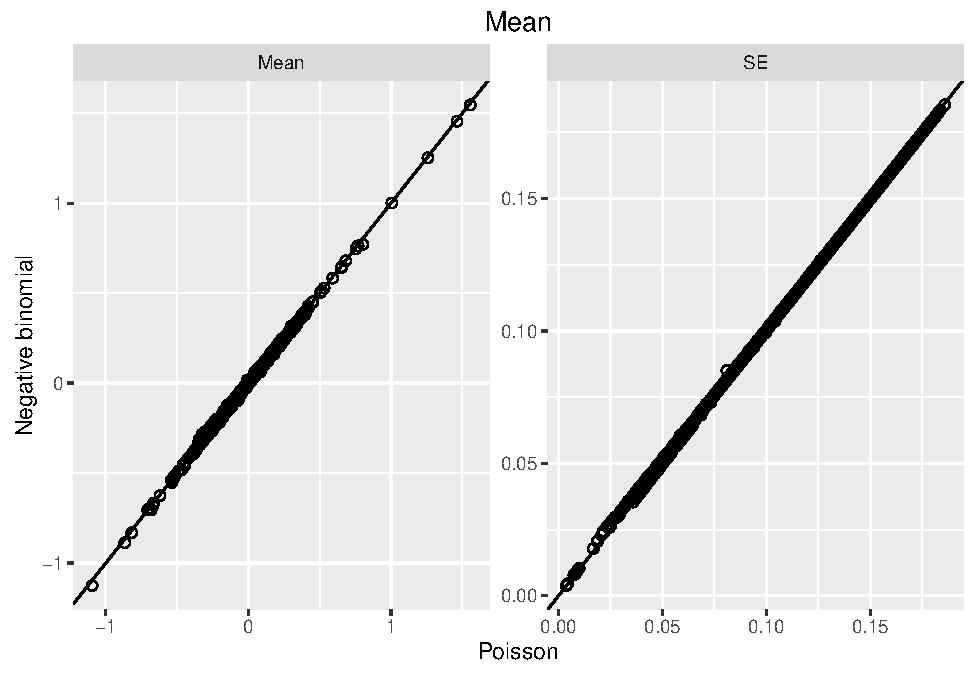
\includegraphics{Thesis_files/figure-latex/male-nbinom-1.pdf}
\caption{Comparison of point estimates and standard errors for men from
Poisson and negative binomial models}
\end{figure}

\begin{figure}[htbp]
\centering
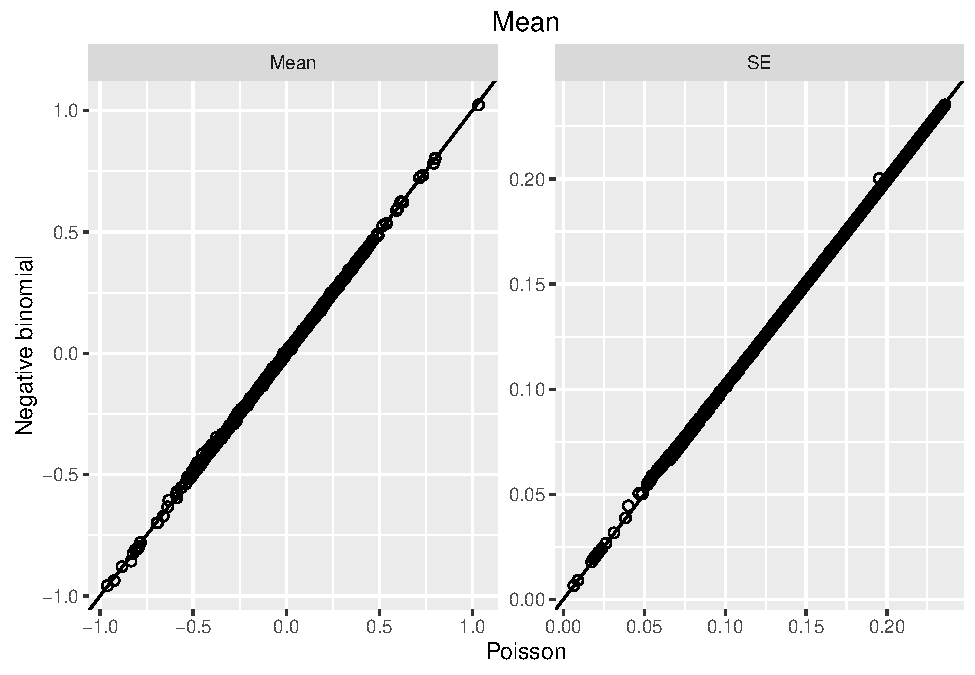
\includegraphics{Thesis_files/figure-latex/female-nbinom-1.pdf}
\caption{Comparison of point estimates and standard errors for women
from Poisson and negative binomial models}
\end{figure}

\begin{figure}[htbp]
\centering
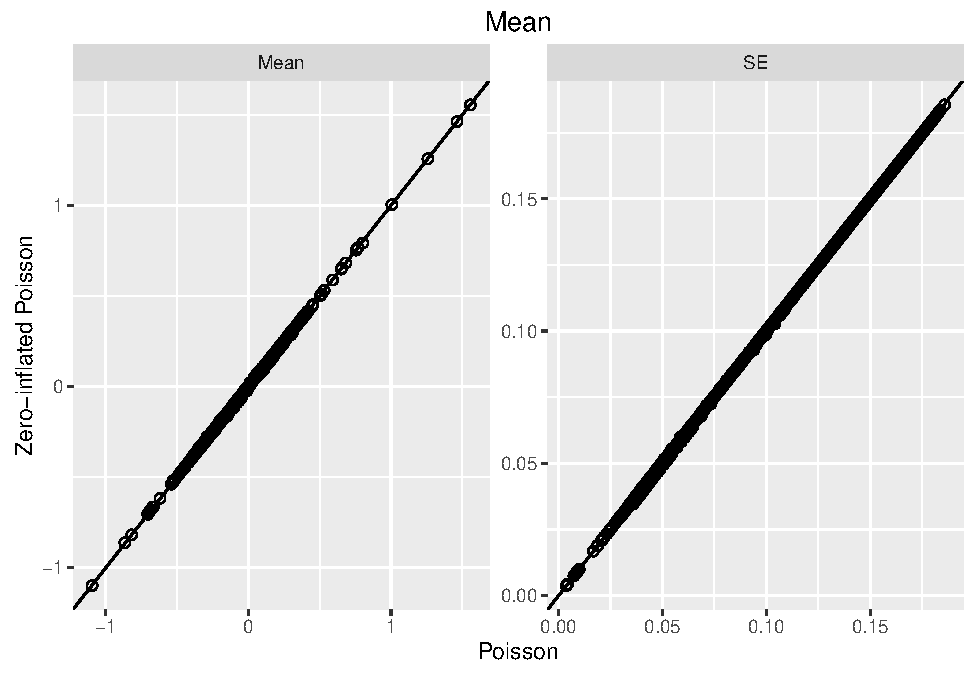
\includegraphics{Thesis_files/figure-latex/male-zipois-1.pdf}
\caption{Comparison of point estimates and standard errors for men from
Poisson and zero-inflated Poisson models}
\end{figure}

\begin{figure}[htbp]
\centering
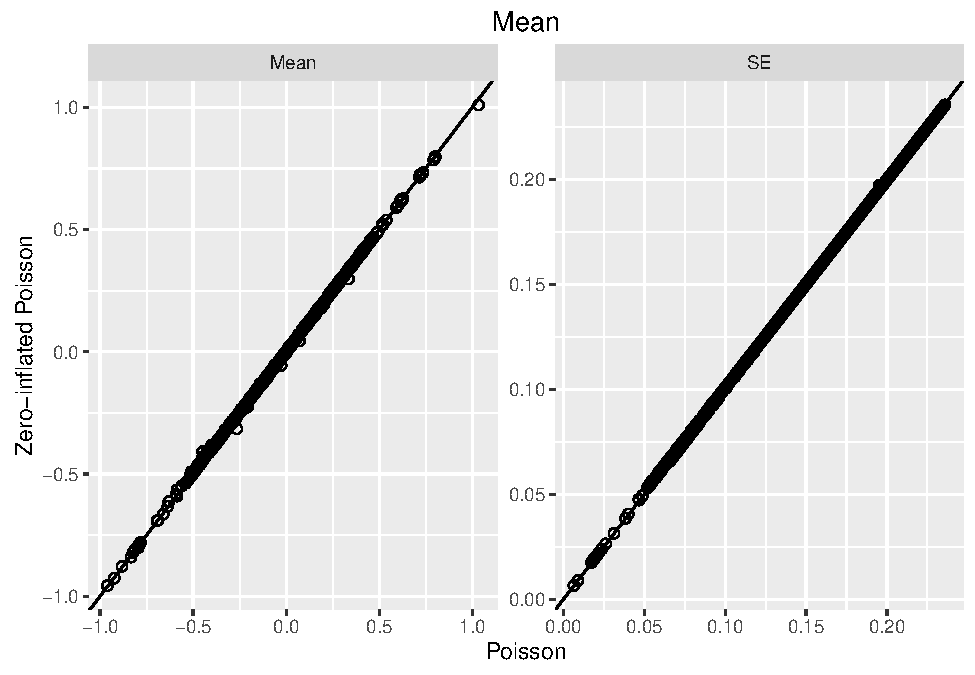
\includegraphics{Thesis_files/figure-latex/female-zipois-1.pdf}
\caption{Comparison of point estimates and standard errors for women
from Poisson and zero-inflated Poisson models}
\end{figure}

\pagebreak

\section*{References}\label{references}
\addcontentsline{toc}{section}{References}

\hypertarget{refs}{}
\hypertarget{ref-herszenhornux5fdemocratsux5f2016}{}
1 Herszenhorn DM, Huetteman E. Democrats end sit-in after 25 hours,
drawing attention to gun control. \emph{The New York Times} 2016;
published online June 23.
\url{http://www.nytimes.com/2016/06/24/us/politics/senate-gun-control.html}
(accessed June 24, 2016).

\hypertarget{ref-barronux5fgunmanux5f2012}{}
2 Barron J. Gunman kills 20 schoolchildren in connecticut. \emph{The New
York Times} 2012; published online Dec 14.
\url{http://www.nytimes.com/2012/12/15/nyregion/shooting-reported-at-connecticut-elementary-school.html}
(accessed June 24, 2016).

\hypertarget{ref-weismanux5fdriveux5f2013}{}
3 Weisman J. Drive for gun control blocked in senate. \emph{The New York
Times} 2013; published online April 17.
\url{http://www.nytimes.com/2013/04/18/us/politics/senate-obama-gun-control.html}
(accessed June 30, 2016).

\hypertarget{ref-ux5fsuicideux5f2016}{}
4 Suicide and self-inflicted injury. National center for health
statistics. 2016; published online Feb 3.
\url{http://www.cdc.gov/nchs/fastats/suicide.htm} (accessed June 30,
2016).

\hypertarget{ref-ux5fallux5f2016}{}
5 All injuries. National center for health statistics. 2016; published
online April 27. \url{http://www.cdc.gov/nchs/fastats/injury.htm}
(accessed Nov 5, 2015).

\hypertarget{ref-ux5fassaultux5f2015}{}
6 Assault or homicide. National center for health statistics. 2015;
published online Feb 6.
\url{http://www.cdc.gov/nchs/fastats/homicide.htm} (accessed June 30,
2016).

\hypertarget{ref-alpersux5ffinlandux5f2015}{}
7 Alpers P, Wilson M. Finland --- gun facts, figures and the law. 2015;
published online Oct 19.
\url{http://www.gunpolicy.org/firearms/region/finland} (accessed Nov 4,
2015).

\hypertarget{ref-alpersux5fcanadaux5f2015}{}
8 Alpers P, Wilson M. Canada --- gun facts, figures and the law. 2015;
published online Oct 19.
\url{http://www.gunpolicy.org/firearms/region/canada} (accessed Nov 4,
2015).

\hypertarget{ref-ux5fbradyux5f2016}{}
9 Brady law. Bureau of alcohol, tobacco, firearms and explosives. 2016;
published online June 23.
\url{https://www.atf.gov/rules-and-regulations/brady-law} (accessed June
24, 2016).

\hypertarget{ref-plumerux5feverythingux5f2012}{}
10 Plumer B. Everything you need to know about the assault weapons ban,
in one post. Washington post. 2012; published online Dec 17.
\url{https://www.washingtonpost.com/news/wonk/wp/2012/12/17/everything-you-need-to-know-about-banning-assault-weapons-in-one-post/}
(accessed June 30, 2016).

\hypertarget{ref-thompsonux5finsleeux5f2016}{}
11 Thompson L. Inslee calls for strengthening background checks of gun
buyers. The seattle times. 2016; published online Jan 6.
\url{http://www.seattletimes.com/seattle-news/politics/inslee-calls-for-strengthening-background-checks-of-gun-buyers/}
(accessed June 30, 2016).

\hypertarget{ref-clarkux5fshortux5f2014}{}
12 Clark M. A short history of chicago's battles with the courts over
gun control. International business times. 2014; published online Jan 7.
\url{http://www.ibtimes.com/short-history-chicagos-battles-courts-over-gun-control-1530100}
(accessed May 13, 2016).

\hypertarget{ref-valentineux5fdisarmed:ux5f2014}{}
13 Valentine M. Disarmed: How cities are losing the power to regulate
guns. \emph{The Atlantic} 2014; published online March 6.
\url{http://www.theatlantic.com/politics/archive/2014/03/disarmed-how-cities-are-losing-the-power-to-regulate-guns/284220/}
(accessed June 30, 2016).

\hypertarget{ref-kellermannux5fgunux5f1993}{}
14 Kellermann AL, Rivara FP, Rushforth NB \emph{et al.} Gun ownership as
a risk factor for homicide in the home. \emph{New England Journal of
Medicine} 1993; \textbf{329}: 1084--91.

\hypertarget{ref-jamiesonux5fgunux5f2013}{}
15 Jamieson C. Gun violence research: History of the federal funding
freeze. American psychological association. 2013; published online Feb.
\url{http://www.apa.org/science/about/psa/2013/02/gun-violence.aspx}
(accessed Nov 5, 2015).

\hypertarget{ref-deniseux5fnoux5f2016}{}
16 Denise M. No, goldie taylor, gun control won't reduce suicide. The
federalist. 2016; published online Jan 12.
\url{http://thefederalist.com/2016/01/12/no-goldie-taylor-gun-control-wont-reduce-suicide/}
(accessed Feb 18, 2016).

\hypertarget{ref-ux5fgunux5f2015}{}
17 Gun control not associated with reducing suicides. NRA-ILA. 2015;
published online Sept 18.
\url{https://www.nraila.org/articles/20150918/gun-control-not-associated-with-reducing-suicides}
(accessed Feb 18, 2016).

\hypertarget{ref-wrightux5fezraux5f2015}{}
18 Wright MA. Ezra klein is wrong: Gun control doesn't reduce suicide
rates. National review online. 2015; published online Aug 27.
\url{http://www.nationalreview.com/article/423192/ezra-klein-wrong-gun-control-doesnt-reduce-suicide-rates-mark-antonio-wright}
(accessed Feb 18, 2016).

\hypertarget{ref-shenassaux5flethalityux5f2003}{}
19 Shenassa ED, Catlin SN, Buka SL. Lethality of firearms relative to
other suicide methods: A population based study. \emph{J Epidemiol
Community Health} 2003; \textbf{57}: 120--4.

\hypertarget{ref-ux5flicensingux5f2016}{}
20 Licensing of owners \& purchasers. Law center to prevent gun
violence. 2016.
\url{http://smartgunlaws.org/gun-laws/policy-areas/gun-owner-responsibilities/licensing-of-owners-purchasers/}
(accessed June 30, 2016).

\hypertarget{ref-websterux5feffectsux5f2014}{}
21 Webster D, Crifasi CK, Vernick JS. Effects of the repeal of
missouri's handgun purchaser licensing law on homicides. \emph{J Urban
Health} 2014; \textbf{91}: 293--302.

\hypertarget{ref-rudolphux5fassociationux5f2015}{}
22 Rudolph KE, Stuart EA, Vernick JS, Webster DW. Association between
connecticut's permit-to-purchase handgun law and homicides. \emph{Am J
Public Health} 2015; \textbf{105}: e49--54.

\hypertarget{ref-crifasiux5feffectsux5f2015}{}
23 Crifasi CK, Meyers JS, Vernick JS, Webster DW. Effects of changes in
permit-to-purchase handgun laws in connecticut and missouri on suicide
rates. \emph{Preventive Medicine} 2015; \textbf{79}: 43--9.

\hypertarget{ref-anestisux5fassociationux5f2015}{}
24 Anestis MD, Khazem LR, Law KC \emph{et al.} The association between
state laws regulating handgun ownership and statewide suicide rates.
\emph{Am J Public Health} 2015; \textbf{105}: 2059--67.

\hypertarget{ref-fleeglerux5fewux5ffirearmux5f2013}{}
25 Fleegler EW, Lee LK, Monuteaux MC, Hemenway D, Mannix R. Firearm
legislation and firearm-related fatalities in the united states.
\emph{JAMA Intern Med} 2013; \textbf{173}: 732--40.

\hypertarget{ref-kposowaux5fimpactux5f2016}{}
26 Kposowa A, Hamilton D, Wang K. Impact of firearm availability and gun
regulation on state suicide rates. \emph{Suicide Life Threat Behav}
2016; published online March 21.
DOI:\href{https://doi.org/10.1111/sltb.12243}{10.1111/sltb.12243}.

\hypertarget{ref-rodriguezux5fandresux5fgunux5f2011}{}
27 Rodríguez Andrés A, Hempstead K. Gun control and suicide: The impact
of state firearm regulations in the united states, 1995--2004.
\emph{Health Policy} 2011; \textbf{101}: 95--103.

\hypertarget{ref-kalesanux5ffirearmux5f2016}{}
28 Kalesan B, Mobily ME, Keiser O, Fagan JA, Galea S. Firearm
legislation and firearm mortality in the USA: A cross-sectional,
state-level study. \emph{The Lancet} 2016; \textbf{387}: 1847--55.

\hypertarget{ref-starkux5fconceptualux5f2011}{}
29 Stark CR, Riordan V, O'Connor R. A conceptual model of suicide in
rural areas. \emph{Rural Remote Health} 2011; \textbf{11}: 1622.

\hypertarget{ref-nationalux5fvitalux5fstatisticsux5fsystemux5fmultipleux5f2013}{}
30 National Vital Statistics System. Multiple cause of death data file,
2013 1980. Centers for Disease Control, 2013.

\hypertarget{ref-worldux5fhealthux5forganizationux5finternationalux5f1977}{}
31 World Health Organization. International classification of diseases,
9th revision. Geneva, Switzerland: World Health Organization, 1977.

\hypertarget{ref-worldux5fhealthux5forganizationux5finternationalux5f1992}{}
32 World Health Organization. International statistical classification
of diseases and related health problems, 10th revision. Geneva,
Switzerland: World Health Organization, 1992.

\hypertarget{ref-ux5fminimumux5f2016}{}
33 Minimum age to purchase \& possess firearms policy summary. Law
center to prevent gun violence. 2016.
\url{http://smartgunlaws.org/minimum-age-to-purchase-possess-firearms-policy-summary/}
(accessed June 14, 2016).

\hypertarget{ref-ux5f2013ux5f2016}{}
34 2013 state scorecard. Brady campaign to prevent gun violence. 2016.
\url{http://www.bradycampaign.org/2013-state-scorecard} (accessed June
30, 2016).

\hypertarget{ref-nra-ilaux5fstateux5f2016}{}
35 NRA-ILA. State gun laws. NRA-ILA. 2016.
\url{https://www.nraila.org/gun-laws/state-gun-laws/} (accessed June 30,
2016).

\hypertarget{ref-ux5fsurveyux5f2016}{}
36 Survey of state procedures related to firearm sales. Bureau of
justice statistics. 2016.
\url{http://www.bjs.gov/index.cfm?ty=dcdetail\&iid=291} (accessed March
25, 2016).

\hypertarget{ref-ux5fgunux5f2016}{}
37 Gun laws in the united states by state. Wikipedia, the free
encyclopedia. 2016; published online April 12.
\url{https://en.wikipedia.org/w/index.php?title=Gun_laws_in_the_United_States_by_state\&oldid=714858022}
(accessed April 12, 2016).

\hypertarget{ref-u.s.ux5fcensusux5fbureauux5ftigerux2flineux5f2015}{}
38 U.S. Census Bureau. TIGER/Line shapefile, 2013 cartographic boundary
file, state-county for united states, 1:20,000,000. U.S. Census Bureau,
2015
\href{https://catalog.data.gov/dataset/2013-cartographic-boundary-file-state-county-forunited-\%20states-1-20000000}{https://catalog.data.gov/dataset/2013-cartographic-boundary-file-state-county-forunited- states-1-20000000}.

\hypertarget{ref-minnesotaux5fpopulationux5fcenterux5fnationalux5f2011}{}
39 Minnesota Population Center. National historical geographic
information: Version 2.0. University of Minnesota, 2011
\url{http://www.nhgis.org}.

\hypertarget{ref-missouriux5fcensusux5fdataux5fcenterux5fcensusux5f2016}{}
40 Missouri Census Data Center. Census summary tape file 3, table NT48A.
MCDC Data Archive (Uexplore/Dexter), 2016
\url{http://mcdc2.missouri.edu/applications/uexplore.shtml}.

\hypertarget{ref-u.s.ux5fcensusux5fbureauux5famericanux5f2016}{}
41 U.S. Census Bureau. American community survey, 2009 american
community survey 5-year estimates, table s1501. U.S. Census Bureau, 2016
\url{http://factfinder2.census.gov}.

\hypertarget{ref-u.s.ux5fcensusux5fbureauux5famericanux5f2016-1}{}
42 U.S. Census Bureau. American community survey, 2010 american
community survey 5-year estimates, table s1501. U.S. Census Bureau, 2016
\url{http://factfinder2.census.gov}.

\hypertarget{ref-u.s.ux5fcensusux5fbureauux5famericanux5f2016-2}{}
43 U.S. Census Bureau. American community survey, 2011 american
community survey 5-year estimates, table s1501. U.S. Census Bureau, 2016
\url{http://factfinder2.census.gov}.

\hypertarget{ref-u.s.ux5fcensusux5fbureauux5famericanux5f2016-3}{}
44 U.S. Census Bureau. American community survey, 2012 american
community survey 5-year estimates, table s1501. U.S. Census Bureau, 2016
\url{http://factfinder2.census.gov}.

\hypertarget{ref-u.s.ux5fcensusux5fbureauux5famericanux5f2016-4}{}
45 U.S. Census Bureau. American community survey, 2013 american
community survey 5-year estimates, table s1501. U.S. Census Bureau, 2016
\url{http://factfinder2.census.gov}.

\hypertarget{ref-u.s.ux5fcensusux5fbureauux5famericanux5f2016-5}{}
46 U.S. Census Bureau. American community survey, 2014 american
community survey 5-year estimates, table s1501. U.S. Census Bureau, 2016
\url{http://factfinder2.census.gov}.

\hypertarget{ref-u.s.ux5fcensusux5fbureauux5fsmallux5f2015}{}
47 U.S. Census Bureau. Small area income and poverty estimates. U.S.
Census Bureau, 2015
\url{https://www.census.gov/did/www/saipe/data/statecounty/data/index.html}.

\hypertarget{ref-u.sux5fbureauux5fofux5flaborux5fstatisticsux5fconsumerux5f2016}{}
48 U.S Bureau of Labor Statistics. Consumer price index: All urban
consumers history, all items 1913-2015. U.S Bureau of Labor Statistics,
2016 \url{http://www.bls.gov/data/}.

\hypertarget{ref-gjertsenux5fmixedux5f2013}{}
49 Gjertsen F, Leenaars A, Vollrath ME. Mixed impact of firearms
restrictions on fatal firearm injuries in males: A national
observational study. \emph{International Journal of Environmental
Research and Public Health} 2013; \textbf{11}: 487--506.

\hypertarget{ref-junuzovicux5funintentionalux5f2012}{}
50 Junuzovic M, Eriksson A. Unintentional firearm hunting deaths in
sweden. \emph{Forensic Science International} 2012; \textbf{216}: 12--8.

\hypertarget{ref-lubinux5fdecreaseux5f2010}{}
51 Lubin G, Werbeloff N, Halperin D, Shmushkevitch M, Weiser M, Knobler
HY. Decrease in suicide rates after a change of policy reducing access
to firearms in adolescents: A naturalistic epidemiological study.
\emph{Suicide Life Threat Behav} 2010; \textbf{40}: 421--4.

\hypertarget{ref-reischux5fchangeux5f2013}{}
52 Reisch T, Steffen T, Habenstein A, Tschacher W. Change in suicide
rates in switzerland before and after firearm restriction resulting from
the 2003 `army XXI' reform. \emph{AJP} 2013; \textbf{170}: 977--84.

\hypertarget{ref-kristensenux5ftmb:ux5f2015}{}
53 Kristensen K, Nielsen A, Berg CW, Skaug H, Bell B. TMB: Automatic
differentiation and laplace approximation. \emph{arXiv:150900660
{[}stat{]}} 2015; published online Sept 2.
\url{http://arxiv.org/abs/1509.00660} (accessed June 30, 2016).

\end{document}
